\documentclass[
%b5paper,  % 默认为 a4paper,根据印刷需求调整
%opensource, % 输出开源信息
decoration,  % 打开装饰
]{qyxf-book}

\title{2020新生手册}
\subtitle{Freshman Handbook 2020}  % 可选
\author{钱院学辅}
\date{2020年8月26日}	
%\typo{AlphaGo}  % 排版人员信息,选填

% 屎山一样的代码,能跑就行
% 感谢编写群群友的宝贵意见,使得文件不断完善

% 定制元信息
%\org{\Large
	%    \textit{加里敦大学}\\
	%    \textsc{Caledon University}
	%}
%\license{}

% 开启 opensource 选项时,以下信息必须填写
% \sourcepage{https://example.com/}


% 使用命令`pandoc v3.0_2020-freshman.docx -o freshman.tex`将Word转为tex
% 排版注:只取.tex文件本行以下内容和pics文件夹
% hypertarget那个不影响功能,是转的时候自动生成的,请无视它
% 页面未调整,但改了些错误
\usepackage{multirow}
\usepackage{graphicx}
\usepackage{multicol}
\usepackage{syntonly}
\usepackage{float}
\usepackage{makecell}
\usepackage{longtable}
\usepackage{caption}
\usepackage{stfloats}
\usepackage{ctex}
\usepackage{ulem}
\usepackage{graphbox}

%\syntaxonly
%\setCJKfamilyfont{zhsong}[simsun.ttc]
\newcommand{\Noto}{\CJKfamily{zhsong}} 

% 面向CSDN编写LaTeX,用于解决LaTeX宋体加粗异常问题,笑死
%\setCJKfamilyfont{zhsong}[AutoFakeBold = {2.17}]{SimSun}
\renewcommand*{\songti}{\CJKfamily{zhsong}}

\graphicspath{{pics}}


\begin{document}
	
	\newcommand\includeFullPageGraphics[2][]{
		\newpage
		\thispagestyle{empty}
		\begin{tikzpicture}[remember picture, overlay, inner sep=0pt]
			\node at (current page.center)
			{\includegraphics[width=\paperwidth, height=\paperheight, keepaspectratio=false,#1]{#2}};
		\end{tikzpicture}
	}
	
	\newcommand{\tightlist}{
		\setlength{\itemsep}{0pt}
		\setlength{\parskip}{0pt}
	}
	
	\includeFullPageGraphics{pics/cover_new.png}
	
	\pagestyle{plain}
	
	\newpage
	\includeFullPageGraphics{pics/qrcode}
	\thispagestyle{empty}
	\mbox{}
	\newpage
	
	\chapter*{致谢}
	感谢各位为本份手册贡献精力的所有同学,他们的付出让本份手册从想法变成了现实,下面列出他们的名字,排名不分先后。
	
	\begin{table}[h]
		\centering
		\begin{tabular}{ccc}
			\multicolumn{3}{c}{\textbf{主编}}\\
			微电子钱91卢嘉骏&越杰91张玉辰&法复001张景怡
		\end{tabular}
		
		\begin{tabular}{ll||ll}
			\multicolumn{4}{c}{\textbf{第一版编者}}\\
			电气713&余希裴&计试71&韩意\\
			数试81&胡兴宇&计算机钱81&刘子宸\\
			电气钱81&赵恒欣&材物81&林睿君\\
			化生81&郭骐瑞&化生81&高旭帆\\
			计试91&李禹陪&钱班92&应昊\\
			钱班93&刘子欣&钱班92&吴弘毅\\
			人工智能91&丁稼宇&越杰91&张玉辰\\
			越杰91&王懿&物试91&张春悦\\
			少年班85&钞\Noto{祎}权&电气钱82&李浩天
		\end{tabular}
		
		\begin{tabular}{ll||ll}
			\multicolumn{4}{c}{\textbf{第二版编者}}\\
			数试001&钞\Noto{祎}权&大数据002&蔡\Noto{彧}彤\\
			数试001&李佳讯&数试002&吴思齐\\
			数试002&李林怿&物试001&丰啸天\\
			物试001&蔡子坚&物试002&张昊东\\
			化生001&张钦&化生001&卢秋宇\\
			人智001&杨进杰&人智91&毕天赐\\
			计试001&苏悦馨&智电钱001&杨艾宸\\
			智电钱001&谭施天一&智电钱001&张雨涵\\
			智能钱001&胡书瑞&智能钱001&桂家彬\\
			自动化钱001&周清扬&自动化钱001&张煜皓\\
			越杰001&赵毓晨
		\end{tabular}
	\end{table}
	
	\newpage
	\begin{table}[h]
		\centering
		\begin{tabular}{ll||ll}
			\multicolumn{4}{c}{\textbf{第三版编者}}\\
			软件2101&郑莲莲&计试2101&胡家铭\\
			自动化钱2101&蔡书阳&力试2101&杨可与\\
			计试001&王思菲&计试2101&杨思成\\
		\end{tabular}
		
		\begin{tabular}{ll||ll}
			\multicolumn{4}{c}{\textbf{第四版编者}}\\
			智电钱2101&曲圣&智造钱2101&范世\Noto{祎}\\
			计试2201&林泽锂&数试2201&李昆岳\\
			宗濂2201&郭颖欣&计试2201&邓博泰\\
			智电钱2201&单靖博&计试2201&李垦\\
			物试2202&蒋金炜&智能钱2201&凌宇韬\\
			基础医学2201&王子洋&数试2201&汤泉宇\\
			力试2201&郑一辰&人智2202&郭鸿铭\\
			越杰2201&王铭正\\
		\end{tabular}

		\begin{tabular}{ll||ll}
			\multicolumn{4}{c}{\textbf{校对}}\\
			智电钱001&王艺斐&物试002&韩煦\\
			宗濂91&白婉婷&能动钱b91&陈智帆\\
			生物技术001&陈昱锦&物试002&肖索源\\
			物试002&刘金昌
		\end{tabular}
		
		\begin{tabular}{ll||ll}
			\multicolumn{4}{c}{\textbf{排版}}\\
			物试001&蔡子坚&物试001&杨尔凡\\
			物试002&韩煦&物试002&张昊东\\
			物试002&武欣格&物试92&祝怀冰\\
		\end{tabular}
		
		\begin{tabular}{ll||ll}
			\multicolumn{4}{c}{\textbf{封面与彩页制作}}\\
			越杰91&张玉辰&自动化92&杜\Noto{昉}宇\\
			物联网001&杨斯涵&大数据002&蔡\Noto{彧}彤\\
			自动化钱2101&高思涵&智电钱2201&单靖博\\
		\end{tabular}
	\end{table}
	
	
	\newpage
	\thispagestyle{empty}
	\mbox{}
	\newpage
	\tableofcontents
	
	\pagestyle{headings}
	
	\chapter{介绍篇}
	\section{钱学森书院简介}
	2016年12月,西安交通大学成立以杰出校友钱学森学长名字命名的“钱学森学院”,同时成立“钱学森书院”,学院与书院合署办公、统一管理,探索双院融合育人模式。钱学森之子钱永刚教授和航天十二院院长薛惠锋教授担任荣誉院长;学院设常务副院长1名,主持钱学森学院工作;副院长1名,负责教学运行工作;书院设院务主任兼党总支书记1名,负责学生管理工作。
	
	学院负责各类拔尖人才培养管理,组织校内外优质教学资源,探索和实践拔尖创新人才培养新模式。学院遵循钱学森教育理念,秉承其大成智慧学中“量智与性质相结合、科学与艺术相结合、逻辑思维与形象思维相结合、微观认识与宏观认识相结合”的思想精髓,面向拔尖学生实施荣誉教育,破格选拔,因材施教,发掘潜能,注重创新,培养学生科学创新能力、综合人文素养和国际视野。
	
	书院负责学生思想政治教育和学生事务管理工作。书院践行“欲成第一学问、事业、人才,须先砥砺第一等品行”的育人思想,传承弘扬“胸怀大局,无私奉献;弘扬传统,艰苦创业”的西迁精神和“爱国、奉献、求真、创新”的钱学森精神,引导学生崇尚科学、勤奋踏实,使学生成为具有社会责任感和家国情怀的“四有青年”。
	
	书院现有包括少年班、工科试验班(钱学森班)、理科试验班(数学、物理、计算机、人工智能)、侯宗濂医学试验班、基础医学拔尖班和越杰班9类拔尖试验班的学生。
	
	西安交通大学作为首批入选国家“基础学科拔尖学生培养试验计划”的高校,于1985年开始招收并培养第一届少年班学生;2007年开办钱学森实验班(2015年更名为工科试验班(钱学森班))和侯宗濂医学实验班;2009年首批入选教育部“基础学科拔尖学生培养试验计划”,开办数学试验班和物理试验班;2016年,开办化学生物试验班和计算机试验班;2018年,开设人工智能试验班和越杰班;2020年开办储能班;2021年数学、物理学、计算机科学、力学、基础医学入选教育部“基础学科拔尖学生培养计划”2.0,同年开办力学试验班和基础医学试验班。目前,西安交通大学各类教育教学改革试点班已经开办三十余年,各类试验班累计招收学生4100余名,培养出2000余名优秀毕业生。
	
	钱学森学(书)院的特殊性不仅体现着前期建设经验中的“特殊人才培养”属性,而且在新的时代环境和背景下,由于自身兼具了书院和学院的合署办公的客观性,将促成人才培养模式向纵深发展。
	
	首先,构建多元化的学生选拔体系,创新试验班选拔方式和水平,学校与学生双向选择,建立学生评估指标和体系,保证各类试验班全面有序开展。同时,为了解决人才选拔培养的多样性与考试招生方式相对单一的矛盾,提出了“兴趣使然、心理健康、学业优秀、体能达标”的德智体综合评价体系,采取高考录取和新生校内选拔相结合的招生模式,积极推进人才选拔模式改革,全面深化人才选拔体制改革。
	
	再次,优化人才培养模式,全面实现人才培养目标。根据各类试验班不同的培养目标,制定特色化培养方案和学生管理办法,并在实施中不断修改完善。一是制定特色课程,努力拓宽学生在人文、艺术、创新思维等方面的知识面。二是建设高水平师资队伍,聘请具有丰富教学经验和国际视野的知名教授担任项目主任,聘任有责任、有能力的青年教师担任班主任。学生的授课教师由最一流的教师担任,并且实施导师制,一个学生配备一位科研导师和一位学业导师,分别侧重学生科研训练的指导和专业学习兴趣的养成。三是学院不断推进国际化建设进程,扩大对外交流与合作,开拓师生的国际化视野,借助国际优质资源,聘请国际知名教授学者授课、讲座报告、交流座谈,培养学生和教师的国际交流能力,鼓励和创造机会让学生出国学习和访问。学院已与美国麻省理工学院、英国曼彻斯特大学、加州大学伯克利分校、新加坡国立大学、佐治亚理工学院等27所世界一流大学签订联合人才培养协议,每年资助近300名本科生赴国外高校交流学习,此项工作已逐步实现规范化、常态化。
	
	最后,书院始终如一的重视拔尖人才爱国主义和家国情怀的培养。书院秉承钱老的名言“Nothing is final”,将其作为院训,激励学生不断努力拼搏,追求卓越,引导学生从大一开始投身学科竞赛、科创活动和科研训练;以“四面旗帜”为引领、“四个一百”活动为抓手,以“西迁精神”和“钱学森精神”作为引导,融入学生成长成才的全过程;以科学与艺术相结合的钱学森教育思想为指导,将第二课堂与第一课堂相结合,开展美育、劳育教育;整合各方优质资源,为学生搭建平台,创办学生刊物《珠峰学报》,培养学生探索科学的精神和创新思维,引导学生投入科研工作,组织开展国际社会实践活动,开阔学生国际视野,拓展学生多元文化四维,培养新时代大学生人类命运共同体责任担当的大局意识;建立多元化学生评价体系,将创新思维、科研训练、研讨参与度等合理地融入到学生考核指标中。建立学生培养档案库,建立拔尖人才选拔—培养—毕业档案库,并长期动态追踪校友毕业后的职业发展,形成完善的信息反馈体系。
	
	钱学森学院和书院深度融合,将教书育人职能和书院制的第二课堂育人有机结合,将成才教育与成人教育无缝衔接,开辟拔尖创新人才培养试验区,发挥教学改革引领示范作用。秉承钱学森大成智慧学中“量智与性质相结合、科学与艺术相结合、逻辑思维与形象思维相结合、微观认识与宏观认识相结合”的思想精髓,培养和造就基础知识宽厚,科学创新能力、综合人文素养和国际视野俱佳的拔尖创新人才。
	
	\noindent 书院官网:http://bjb.xjtu.edu.cn/index.htm\\
	办公地点:仲英楼(材料与基础学科大楼)B座9楼\\
	钱学森书院官方网址:http://bjb.xjtu.edu.cn/xygk/zzfg.htm\\
	
%	\begin{figure}[htbp]
%		\centering
%		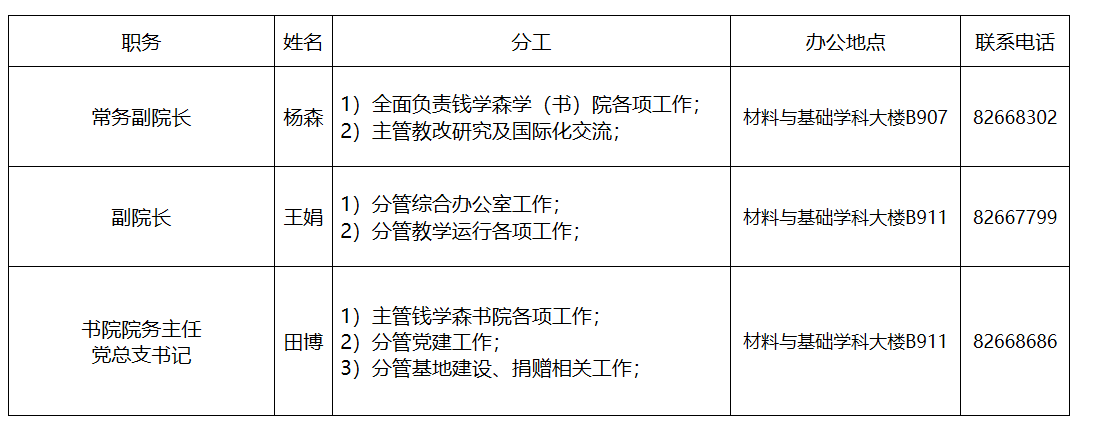
\includegraphics[width=1.0\linewidth]{pics/sheet.png}
%	\end{figure}

	\begin{table}[h]
	\small %此处写字体大小控制命令
	\begin{tabular}{ | c | c | c | c | c |}
		\hline
		职务 & 姓名 & 分工 & 办公地点 & 联系电话 \\
		\hline
		常务副院长 & 杨森 & \makecell{1. 全面负责钱学森学(书)院各项工作;\\2. 主管教改研究及国际化交流;} & 材料与基础学科大楼B907 & 82668302 \\
		\hline
		副院长 & 王娟 & \makecell{1. 分管综合办公室工作;\\2. 分管教学运行各项工作;} & 材料与基础学科大楼B911 & 82667799 \\
		\hline
		\makecell{书院院务主任\\党总支书记} & 田博 & \makecell{1. 主管钱学森书院各项工作;\\2. 分管党建工作;\\3. 分管基地建设、捐赠相关工作;} & 材料与基础学科大楼B907 & 82668686 \\
		\hline
	  \end{tabular}
	\end{table}

%	\begin{figure}[htbp]
%		\centering
%		
\includegraphics[width=4cm]{pics/2023.jpg}
%		\setlength{\abovecaptionskip}{0.0cm}
%		\setlength{\belowcaptionskip}{0.2cm}
%		\caption*{2023级钱学森书院新生群}
%		\end{figure}
	
	\section{学辅简介}
	钱学森书院学业辅导中心(简称“钱院学辅”)是一个面向全校的朋辈辅导机构,欢迎各年级、各书院的同学加入我们!
	
	在这里,我们有:幽默活泼的答疑群、精美实用的学习资料、精益求精的志愿者团队!
	
	来到这里,你可以:获得新的技能、拥有最好的学习氛围、收获一批志同道合的伙伴、在分享与被分享中不断提升自己!
	
	学辅下设五个部门,下面将依次介绍:
	
	\textbf{主创团}负责统筹安排学辅各部门的工作与活动,为钱院学辅的运营“保驾护航”!
	
	现任主任:智电钱2101曲圣、智造钱2101范世\Noto{祎}
	
	\textbf{学研部}负责资料的整理编写、答疑工作的安排以及志愿者的统筹。
	
	现任部长:计试2201林泽锂、数试2201李昆岳
	
	钱院学辅学研部的核心工作之一,在于资料的编写,目前学辅的资料有《大学物理题解》、《理论力学习题解答》、《钱班专业分流指南》、《实变习题解答》和《仪器分析提纲》等多部精美学习资料,学辅所编写的所有资料可在钱院学辅信息站(https://qyxf.site/)上查找,或者加入钱院学辅交流分享群,群号及二维码在本章末尾,从群文件中下载。
	
	开展讲座也是学研部的工作重点,在过去的一年里,学研部负责举办了如出国交流分享会、LaTeX排版讲座、理论力学期末复习讲座、寒假科研入门培训系列讲座以及钱学森班专业分流讲座等多次讲座,均反响良好。
	
	此外,学研部还在运营着日常答疑群——科研经验交流群即科粉群。
	
	\textbf{宣传部}负责微信公众号的运营、活动海报的设计以及学辅相关活动的组织运营等工作,并且承担《珠峰学报》和《迎新手册》等资料的封面设计工作。
	
	现任部长:人智2101陈智、计试2201任真
	
	部门特色:
	
	1.可以学到实用的技能,学习制作推送,感受自主设计创造的快乐。
	
	2.鼓励大家尝试各类宣传途径,激发同学的创新精神。
	
	3.任务分配合理,成员参与度高,同时任务量较少便于协调学业。
	
	4.充足的志愿工时,激励成员追求更高质量的完成宣传工作。
	
	\begin{figure}[htbp]
		\centering
		\begin{minipage}{4cm}
			
\includegraphics[width=4cm]{pics/zf.png}
		\end{minipage}
		\begin{minipage}{4cm}
			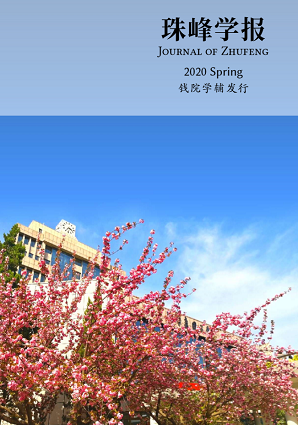
\includegraphics[width=4cm]{pics/zf1.png}
		\end{minipage}
		\begin{minipage}{4cm}
			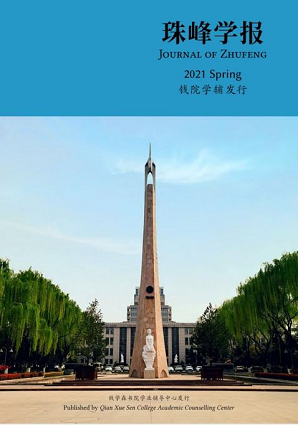
\includegraphics[width=4cm]{pics/zf2.png}
		\end{minipage}
	\end{figure}
	
	\textbf{办公室}负责学辅内部筹办各种活动以及工时的认定等,并且协助学研部玩完成讲座开展的相关事宜,并且会与钱学森书院学生会联合举办活动,如中秋游园会、元旦游园会等。
	
	现任部长:宗濂2201郭颖欣、计试2201邓博泰
	
	\textbf{《珠峰学报》编辑部}负责《珠峰学报》的征稿、编辑和审稿工作,截止2020年8月,已经出版过两期。
	
	\textbf{钱学组}全称钱班学习分享小组,是下属于学研部的独立部门,是自2020级起钱班内部通过整理学习资料、举办课程辅导讲座以帮助同学们学业进步的学习性小组。
	
	钱学组的核心工作是资料编写。自2020-2021学年第二学期起,钱学组编写了多份涵盖各个学科的课程学习资料,其中《高数积分习题整理》《国防教育知识点》《有机化学期末模拟试题》《17年大物阶段2试题参考答案》等在当时填补了合适有效的复习资料空缺,获得了同学们的广泛好评。

	
	\begin{figure}[h]
		\centering
		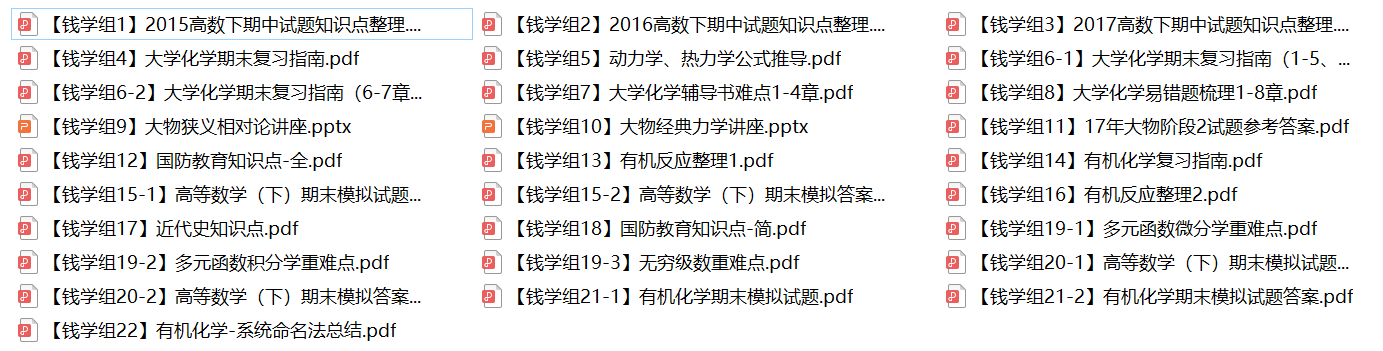
\includegraphics[width=0.6\linewidth]{pics/qianxuezu01.png}
	\end{figure}
	
	与此同时,钱学组也根据同学们需要举办了多场讲座。钱学组曾举办有关工科数学分析学习辅导、大学化学学习辅导、工程图学学习辅导、大学物理学阶段考试备考、大学生英语竞赛备考、美国大学生数学建模竞赛备赛的讲座,取得了良好的效果。
	
	\begin{figure}[h]
		\centering
		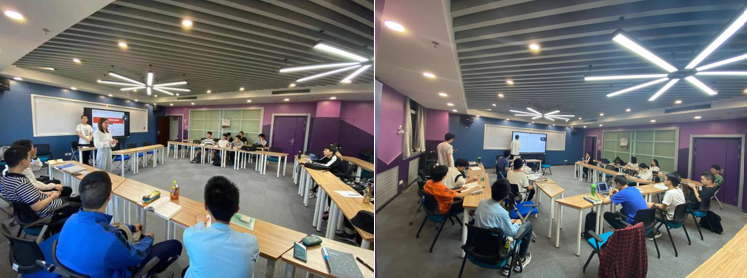
\includegraphics[width=0.6\linewidth]{pics/qianxuezu02.png}
	\end{figure}
	
	这里主要会办理寒暑假的请假销假手续。请销假一般只是走个流程。校外机动车入校等服务也是这里登记。

	\textbf{计学组}全称计试思博伴学小组,是自2020级起计试班级内部发起的互助性学习小组。计学组的核心工作是整理学业资料、开展答疑活动、举办分享讲座。资料方面,经过计试各年级同学的共同努力,整理编辑了程序设计基础、数据结构与算法、神经生物学等课程的复习资料,总结形成了保研经验分享等宝贵的经验文件,很好地补充了计试在这方面的资料空缺情况。答疑方面,在辅导员老师的支持下,在钱院学辅的指导下,计学组在考前联合多个试验班开展了公选课共同答疑+特色课单独辅导的答疑模式,通过线上+线下的答疑方式,有效统筹利用了学辅内部的资源,取得了较好的效果。讲座方面,通过开展高数学习体会分享讲座、竞赛经验交流讲座等多场讲座活动,收获了参会者的一致好评。

	\subsection{我们的联系方式}
	
	·招新报名表:
	\begin{figure}[H]
		\centering
		
\includegraphics[width=0.35\linewidth]{pics/1111111111.jpg}
	\end{figure}
	·招新群:
	\begin{figure}[H]
		\centering
		
\includegraphics[width=0.35\linewidth]{pics/222222222.jpg}
	\end{figure}
	·“钱院学辅”公众号:
	在订阅号中搜索“钱院学辅”
	或扫描二维码:

	\begin{figure}[H]
		\centering
		
\includegraphics[]{33333333333.png}
	\end{figure}
	
	\section{钱学森书院团工委简介}
	想进一步了解共青团吗?想近距离接触团学工作吗?快来加入钱院团工委!
	
	\subsection{我们的简介}
	
	\textbf{共青团西安交通大学钱学森书院工作委员会(以下简称钱院团工委)}成立于2016年,是由校团委派出至钱学森书院的代表机关,负责钱学森书院各学生组织和各团支部的思想政治工作,主要从事团学组织与策划、志愿服务及社会实践开展、科创竞赛指导、党团新媒体建设路径探索等工作,是书院与书院内其他组织的桥梁与纽带。
	
	\textbf{2021至2022学年},为了进一步提高钱院团工委工作质量、更好地开展各项工作,第六届团工委鉴于所负责工作的特点及差异性,将实践中心分划为社会实践中心、志愿服务中心、科创中心三个独立的部门。\textbf{第六届团工委由团组织建设指导中心、社会实践中心、志愿服务中心、科创中心以及新媒体中心五个部门组成。}为了更好地开展各项工作、提高工作质量、补充新鲜血液,\textbf{现拟招若干名干事,欢迎踊跃报名!}
	
	\subsection{我们的特色}
	钱学森书院团工委是我校各书院中最年轻的共青团工作委员会。其成员全部来自各类理工科试验班,具有高学科素养,更具有学科特色。钱学森书院团工委充分利用这一特点,致力于打造出一支具有各学科交叉思维的团队。同时,团工委也注重人文政治思想的培养,开展主持开展各类活动,着力打造出一支具有人文素养的团队。
	
	
	\begin{itemize}
		
		\item 钱学森日
			\begin{figure}[H]
        		\centering
        		\begin{minipage}{4cm}
        		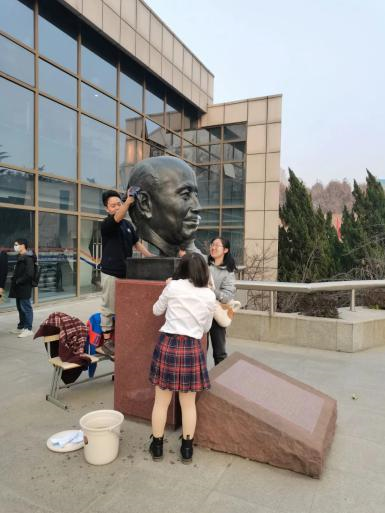
\includegraphics[width=4cm]{pics/qxsr1.png}
        		\end{minipage}
        		\begin{minipage}{4cm}
        		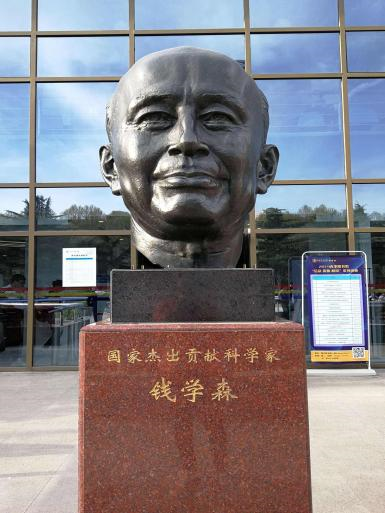
\includegraphics[width=4cm]{pics/qxsr2.png}
        		\end{minipage}
				\begin{minipage}{7.3cm}
        		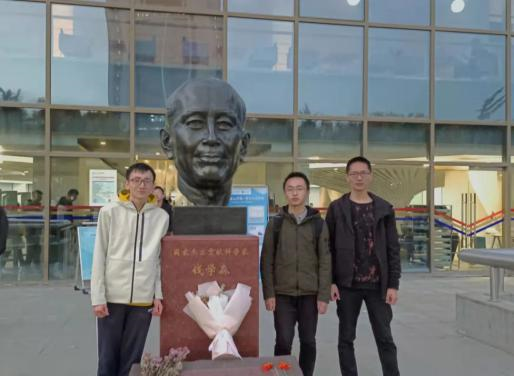
\includegraphics[width=7.3cm]{pics/qxsr3.png}
				\end{minipage}
        	\end{figure}
		
		\item 最佳团日
		\begin{figure}[H]
			\centering
			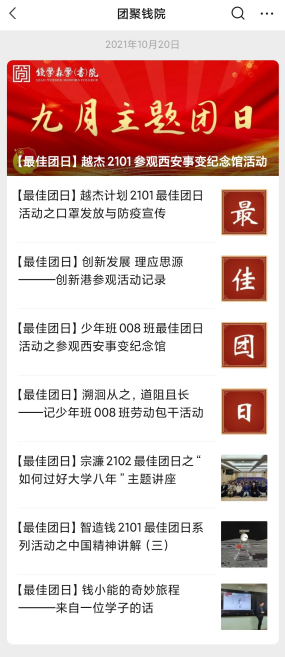
\includegraphics[]{pics/zjtr.png}
			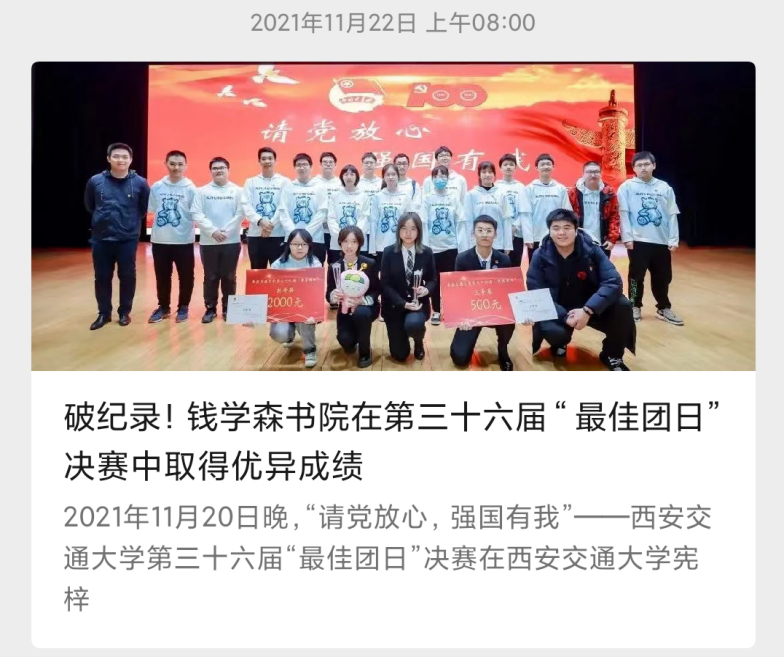
\includegraphics[]{pics/zjtr1.png}
		\end{figure}
	\end{itemize}
	
	\begin{itemize}
		\item 少年班成人礼\& 书院荣誉毕业典礼
	\end{itemize}
	\begin{figure}[H]
		\centering
		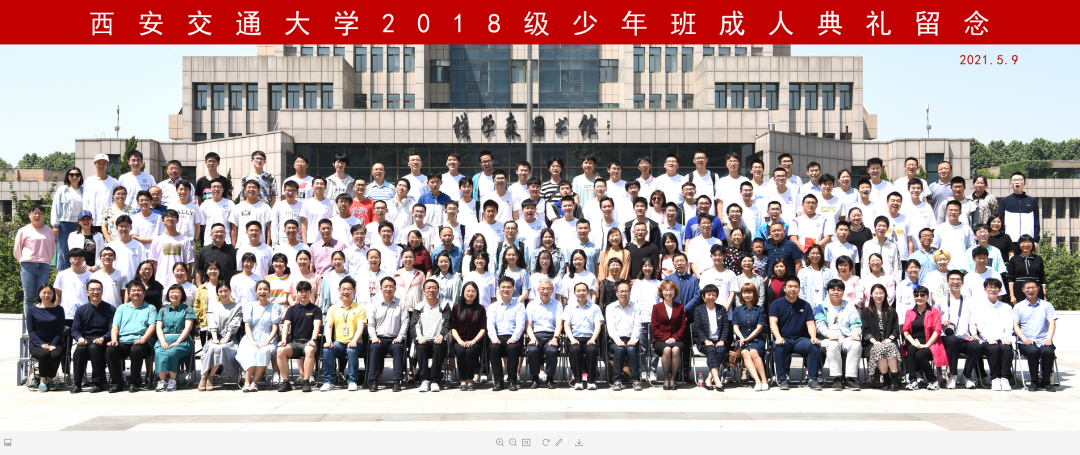
\includegraphics[width=0.6\linewidth]{pics/tuan05.png}
	\end{figure}
	\begin{figure}[H]
		\centering
		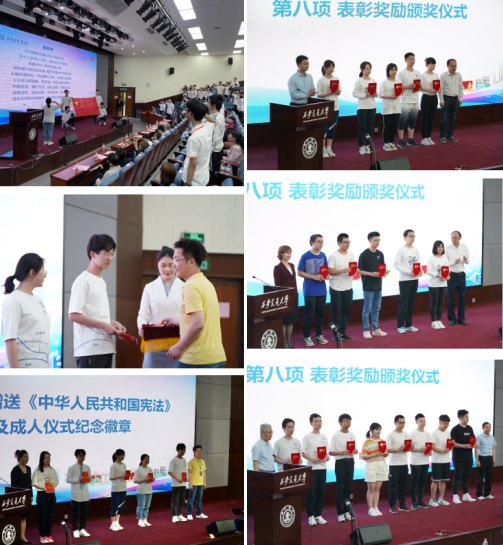
\includegraphics[width=0.6\linewidth]{pics/tuan06.png}
	\end{figure}
	
	\begin{itemize}
		\item 十四运
	\end{itemize}
	
		\begin{figure}[H]
			\centering
			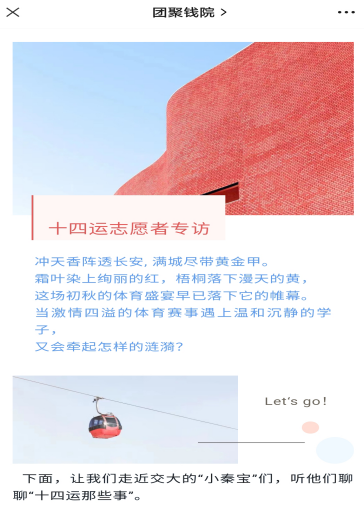
\includegraphics[scale=1.4]{pics/sxy1.png}
			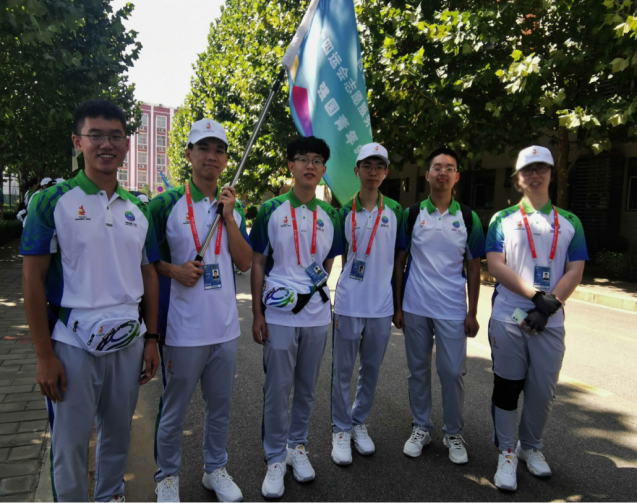
\includegraphics[scale=1.4]{pics/sxy2.png}
		\end{figure}
	
	
	\begin{itemize}
		\item 社会实践、腾飞杯竞赛等的宣传、报名与审核
	\end{itemize}
	
			\begin{figure}[H]
        		\centering
        		\begin{minipage}{5cm}
        		
\includegraphics[]{pics/shsj1.png}
        		\end{minipage}
        		\begin{minipage}{5cm}
        		
\includegraphics[]{pics/shsj2.png}
        		\end{minipage}
				\begin{minipage}{5cm}
				
\includegraphics[scale=0.8]{pics/shsj3.png}
				\end{minipage}
        		\end{figure}
		
	\begin{itemize}
		\item 政府见习,五四表彰,民生大侦探……
	\end{itemize}
	
	\begin{figure}[H]
		\centering
		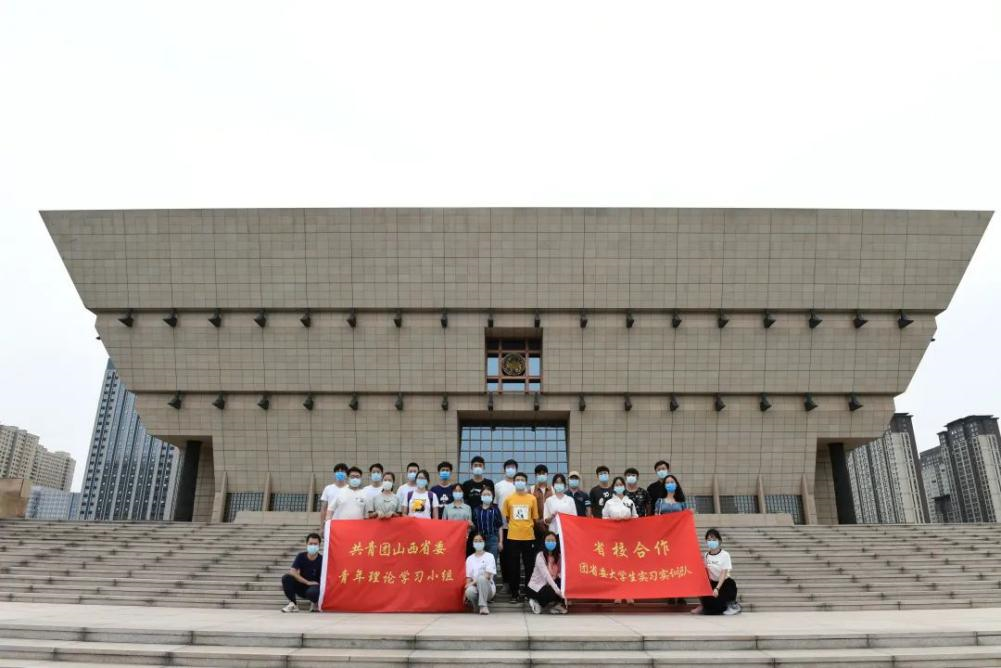
\includegraphics[]{pics/gdhd.png}
		\caption*{(政府见习|西交学子赴山西省参与党政学习)}
	\end{figure}
	
	
	\subsection{我们的部门}
	
	\begin{enumerate}
		\item 团组织建设指导中心
		\begin{itemize}
			\item
			联系校团委与各团支部,发挥上传下达的工作职能。
			\item
			负责团籍注册、新团员发展、推优入党工作。
			\item
			管理和指导团组织生活会,组织策划团支书培训,负责 “最佳团日”活动的组织申报、活动指导,开展团日活动的经验交流、样例示范工作。
			\item
			负责各团支部团支书的考评工作。
		\end{itemize}
		\item 社会实践中心
		\begin{itemize}
			\item
			策划社会实践活动开展,在组队、项目选择、项目宣传方面进行支持,谋求建立具有钱院团工委特色的社会实践活动。
		\end{itemize}
		\item 志愿服务中心
		\begin{itemize}
			\item
			组织策划志愿活动
			\item
			负责志愿者招募、培训和日常管理工作
			\item
			建立与志愿活动来源的长期合作关系
		\end{itemize}
		\item 科创中心
		\begin{itemize}
			\item 与钱学森书院学业辅导中心合作,对各类科创竞赛(包括腾飞杯、挑战杯、互联网 +、大创)的组队、项目选择、朋辈交流工作进行部署。
		\end{itemize}
		\item 新媒体中心
		\begin{itemize}
			\item
			运营团工委公众号“团聚钱院”,QQ号钱小团,负责活动宣传及团员日常思想引领。
			\item
			开展多媒体技术讲座,传播公众号排版、运营知识,发掘培养更多优秀人才。
			\item
			进行海报、公众号宣传图等平面设计工作,以及视频剪辑、制作等相关工作。
		\end{itemize}
	\end{enumerate}
	
	\subsection{在这里,你能收获什么}
	
	
	在钱院团工委的大家庭中,你会在轻松的氛围中,收获组织活动的工作经验,学会如何协调各类事情;在钱院团工委开展的一系列特色活动中,你会在学习之余体验到大学生活的乐趣;在钱院团工委为你提供的展示自我的平台上,你能接触各类试验班的优秀同学,交到更多的朋友,同时还能够提高自身人文素养。
	
	\begin{itemize}
		\item 培养业务管理、团队协作、沟通交流等能力,全面提升自我
		\item 深度参与团组织的工作,积累工作经验,提升自我价值
		\item 参与志愿活动和社会实践项目的管理,得到更多实践的机会和经验
		\item 深入了解各类科创竞赛,掌握一手信息
		\item 学习平面设计、公众号运营等技能,增长自我才干
		\item 结识一群志同道合的伙伴
		\item ……
	\end{itemize}
	
	\subsection{我们的联系方式}
	
	·钱小团:
	\begin{figure}[H]
		\centering
		
\includegraphics[width=0.35\linewidth]{pics/tuan14.jpg}
	\end{figure}
	·招新群:
	\begin{figure}[H]
		\centering
		
\includegraphics[width=0.35\linewidth]{pics/tuan15.jpg}
	\end{figure}
	·“团聚钱院”公众号:
	在订阅号中搜索“团聚钱院”
	
    并找到如下图标

	\begin{figure}[H]
		\centering
		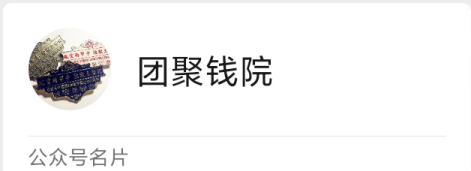
\includegraphics[]{tjqy.png}
	\end{figure}

	\section{钱学森书院学生会简介}
	
	\begin{figure}[htbp]
		\centering
		
\includegraphics[width=4cm]{pics/qyxsh_logo.png}
		\setlength{\abovecaptionskip}{-0.2cm}
		\setlength{\belowcaptionskip}{0.2cm}
		\caption*{钱院学生会logo}
	\end{figure}
	
	钱学森学(书)院学生会于2018年9月成立,是西安交通大学学生会的分会之一,也是西安交通大学学生会中最年轻的学生分会。
	
	与按照兴趣聚集成的社团不同,学生会是党领导下的主要学生组织,坚持“全心全意为同学服务”的宗旨。钱学森学(书)院学生会在钱学森书院党总支的领导、团工委的指导下开展各项工作,聚焦书院同学精神成长、学习生活、权益服务等各方面需求,举办适合钱院青年学生特点的文化、科技、体育、学习类活动,关心同学们的学习、工作和生活,是书院联系广大同学的桥梁和纽带。
	
	目前,钱院学生会共设有五个部门,为办公室、体育部、外联部、宣传部、文化部。
	
	\begin{figure}[htbp]
		\centering
		
\includegraphics[width=8cm]{pics/wechater.png}
		\setlength{\abovecaptionskip}{0.0cm}
		\setlength{\belowcaptionskip}{0.2cm}
		\caption*{钱院学生会微信公众号}
	\end{figure}
	
	\subsection{精品活动介绍}
	
	\subsubsection{“钱与钱寻”}
	在每年的钱学森日(12月11日)附近,钱院学生会都会开展“钱与钱寻”钱学森粉丝资格考试(原“钱学森日”主题活动),号召钱院乃至全校同学通过游戏等多种多样的方式了解钱老生平、感悟钱学森精神。
	
    “钱与钱寻”活动让同学们在欢声笑语中了解钱老光荣奉献的一生,体会钱老对交大学子的殷殷期盼,明白自己身上肩负的责任,使同学们在放松之余也有所收获。
    
	\begin{figure}[htbp]
		\centering
		\begin{minipage}{6cm}
		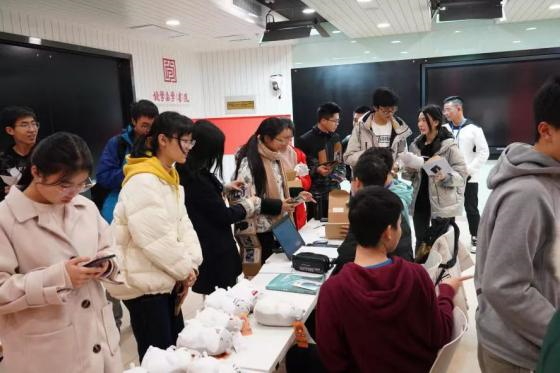
\includegraphics[width=6cm]{pics/qyqx1.png}
		\end{minipage}
		\begin{minipage}{6cm}
		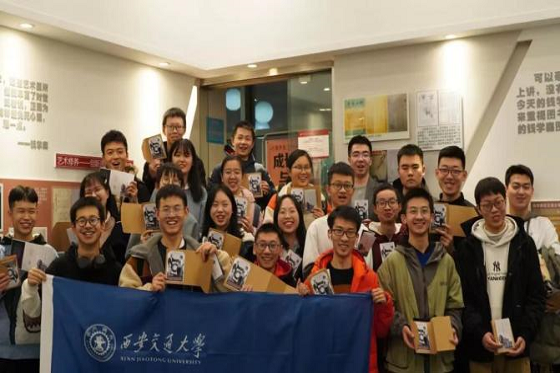
\includegraphics[width=6cm]{pics/qyqx2.png}
		\end{minipage}
	\end{figure}
	
	\subsubsection{国庆“星”计划}
	国庆“星”计划,即在国庆节期间,两名学长学姐与两名新生自由组合或根据兴趣随机匹配为一组,共同完成自习、运动、逛校园、探秘食堂、爬秦岭、密室逃脱、剧本杀等各种活动以获取星星、兑换奖品。本活动旨在帮助新同学在学长学姐的指导下,快速适应校园学习生活。本活动于2021年第一次举办,同学们反响相当热烈。
	
	\begin{figure}[h!]
		\centering
		\begin{minipage}{5cm}
		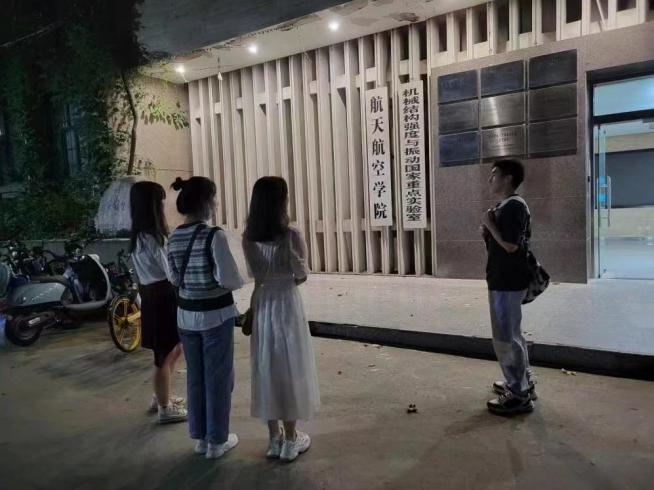
\includegraphics[]{pics/gqxjh1.png}
		\end{minipage}
		\begin{minipage}{5cm}
		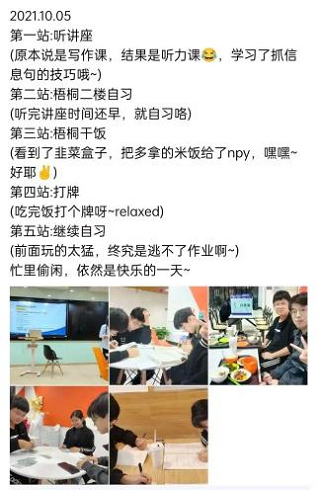
\includegraphics[]{pics/gqxjh2.png}
		\end{minipage}
	\end{figure}
	
	\subsection{各部门介绍}
	
	\subsubsection{办公室}
	办公室=听会+协调+起草文件?
	
    NO! Far more than that!
    
    在办公室,你不仅可以体验上面办公室的常规工作,还可以Hold住钱院学生会的财务大(xiao)权,举办活动,丰富课余生活的同时找到志同道合的朋友,扩大你的圈子。
    
    作为历届学生会中男女比例最均衡的部门,不妨考虑努努力、在这里顺便、一不小心解决一下情感问题?
    
    办公室丰富多彩,但这还不够!在办公室,只要你有好点子、想为同学做事,我们就会全力支持,让你体会到大份量的满足和成长。
    
    期待办公室的未来,有你!

	\begin{figure}[htbp]
	\centering
	
\includegraphics[width=4cm]{pics/officeqrcode.png}
	\setlength{\abovecaptionskip}{0.0cm}
	\setlength{\belowcaptionskip}{0.2cm}
	\caption*{办公室详细介绍}
	\end{figure}
	
	\subsubsection{体育部}
	文明其精神,野蛮其体魄!
	
    钱学森书院学生会体育部致力于钱院学子体育精神之灌注,身体素质之构筑,竞技水平之炼铸!过去一年中,体育部统筹协调书院各项体育运动,得到了钱院学子广泛响应。钱院学子在各项体育竞技赛事中奋勇争先,屡获佳绩:篮球新生杯勇夺季军,运动会团体总分位列全校第三!过去的一年,我们突破历史,在各项校级赛事中获得书院的历史最佳成绩;新的一年,期望你我共创历史:书院游泳队的创立、新生杯与运动会的再创佳绩、钱院学子体测水准的再攀高峰……
    
    我们将一同见证,属于我们钱院人的历史!加入钱院体育部,共做历史的开拓者!
	\newpage
	\begin{figure}[htbp]
		\centering
		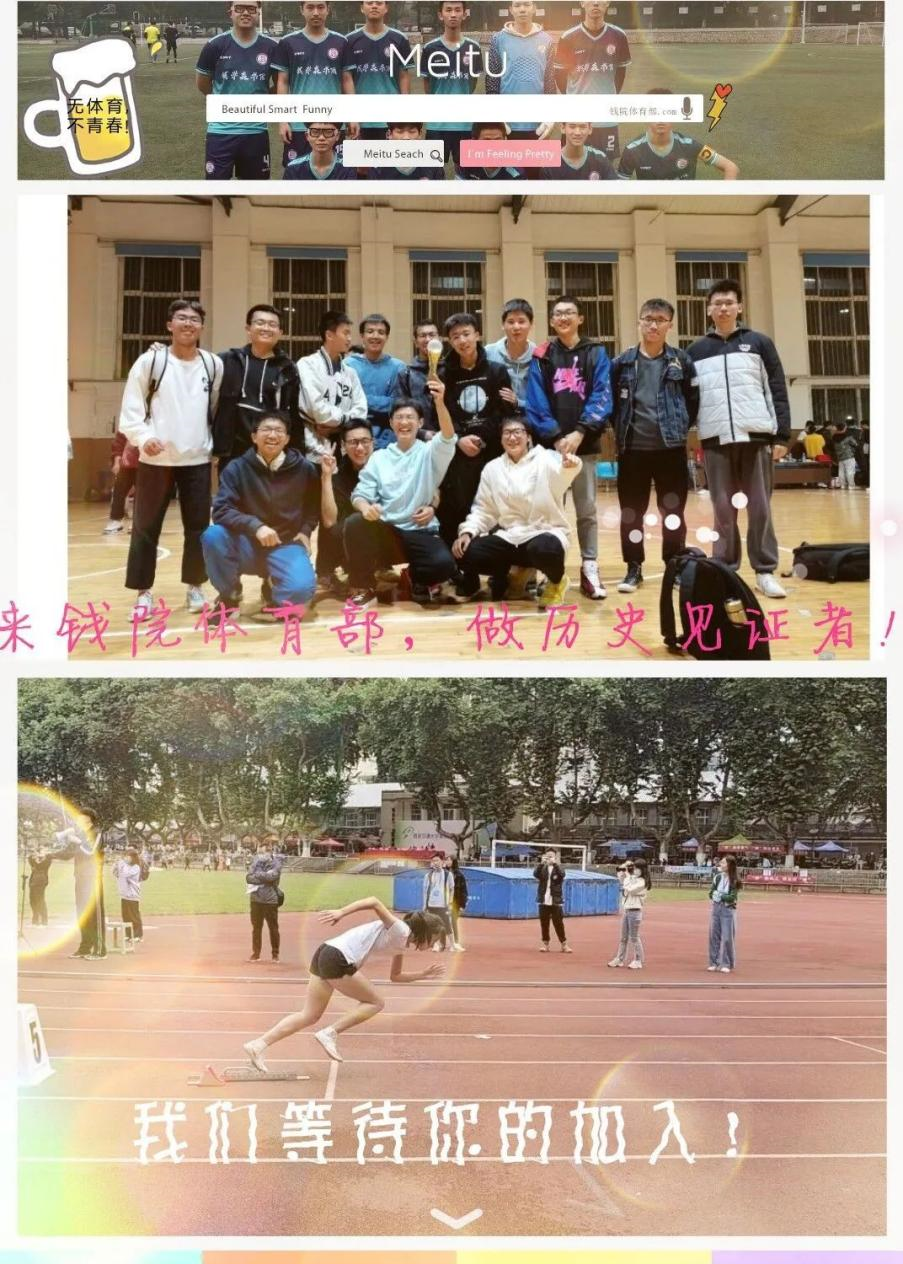
\includegraphics[align=c,width=5cm]{pics/gym.png}
		\end{figure}

	\begin{figure}[htbp]
	\centering
	
\includegraphics[align=c,width=4cm]{pics/gymqrcode.png}
	\vspace{-2cm}
	\setlength{\abovecaptionskip}{2cm}
	\setlength{\belowcaptionskip}{1cm}
	\caption*{体育部详细介绍}
	\end{figure}

	
	\subsubsection{外联部}
	外联部作为学生会下属的重要部门,是学生会的对外窗口,也是外界了解钱院学生会的直接途径。
	
    外联部也同时肩负着联络校内外各组织、志愿者管理、活动策划、迎新等工作,是提升工作能力、交流沟通能力、组织能力的不二之选。
    
    在这里,大家不仅讨论着日常的活动安排、工作事项,还可以互相加深了解,成为大学学习生活的好伙伴,组织活动时还可以结识很多新朋友。
    来实践美好的大学生活吧,外联部大家庭欢迎你的加入!

	\begin{figure}[htbp]
		\centering
		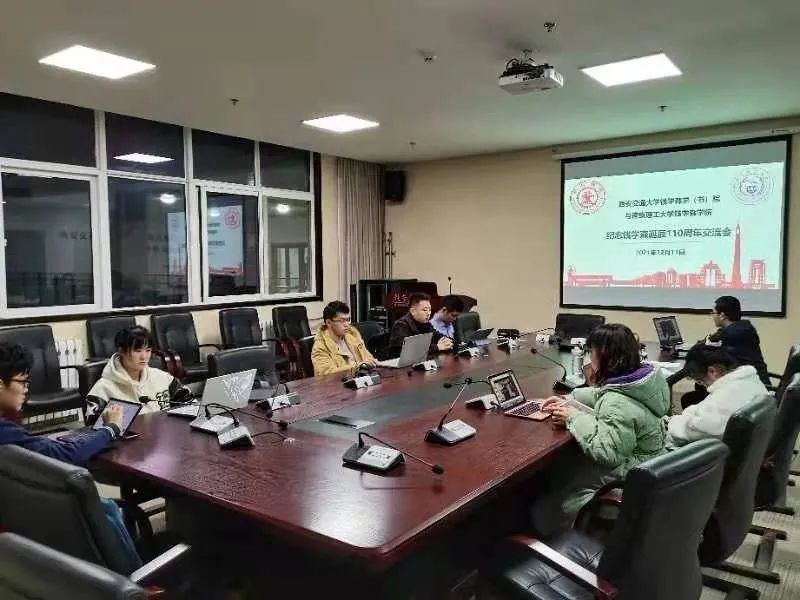
\includegraphics[width=6cm]{pics/wlb.png}
	\end{figure}


	\begin{figure}[htbp]
	\centering
	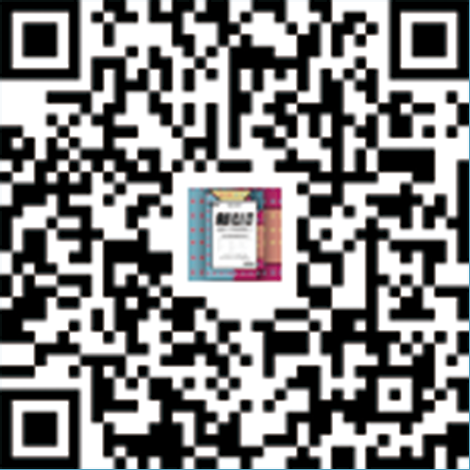
\includegraphics[width=4cm]{pics/wlbqrcode.png}
	\setlength{\abovecaptionskip}{0.0cm}
	\setlength{\belowcaptionskip}{0.2cm}
	\caption*{外联部详细介绍}
	\end{figure}	
		

	\subsubsection{宣传部}
	如果现在给你一台电脑,你脑海中第一下闪过的片段是什么?
	
    游戏,刷剧,又或者是聊天?NO! NO! NO!
    
    你可以试试让它发挥些特别的作用?比如设计一张海报,比如剪辑一段视频,或者完成一次排版!担心自己是电脑小白不懂操作?没关系!我们会有相关技术人员进行专业指导。你还可以根据自己的兴趣爱好自主选择分组。渴望你们的加入,在钱院宣传部这个大家庭里书写属于你们的故事!

	\begin{figure}[htbp]
	\centering
	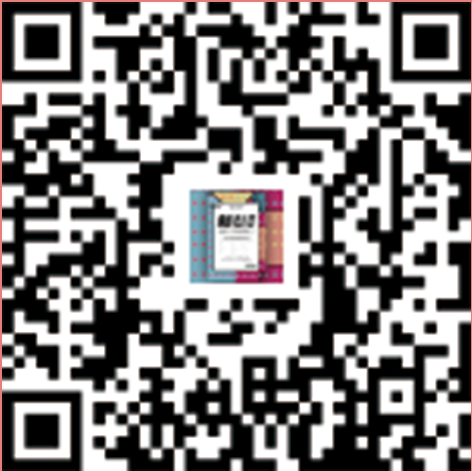
\includegraphics[width=4cm]{pics/xcb.png}
	\setlength{\abovecaptionskip}{0.0cm}
	\setlength{\belowcaptionskip}{0.2cm}
	\caption*{宣传部详细介绍}
	\end{figure}	
    	
	\subsubsection{文化部}
	从西瓜游行到学习伴侣,从中秋佳节到元旦跨年,举办多彩的文艺活动是我们的职责所在。在给同学们带来有趣活动的同时,我们更能从活动策划与工作筹备中获得独特的体验与快乐。我们也聚焦于钱学森学院同学的学习生活与权益服务,既引领着钱院寝室文化的建设,也倾听同学们的烦恼,为学生代表大会收集宝贵的意见。
	
    在接下来的一年里,文化部愿与你同行,用绚丽的色彩涂抹钱院er的生活,让你我的心声回响青春的校园。
	\newpage
	\begin{figure}[htbp]
		\centering
		
\includegraphics[align=c,width=5cm]{pics/whb.png}
		\end{figure}

	\begin{figure}[htbp]
	\centering
	
\includegraphics[align=c,width=4cm]{pics/whbqrcode.png}
	\vspace{-2cm}
	\setlength{\abovecaptionskip}{2cm}
	\setlength{\belowcaptionskip}{1cm}
	\caption*{体育部详细介绍}
	\end{figure}
	
	\subsection{招新}
	各位优秀的钱院学子,请看过来!
	
    欢迎大家成为钱学森书院大家庭的一份子,在这里迈入自己人生的全新阶段,揭开丰富多彩的大学生活的帷幕。而大学想要过得充实饱满,怎么能少得了各式各样的社团活动和学生组织?如果你尚且心存疑虑,不知作何选择,不妨来听听我们的建议——
    
    如果你是这样的:
    
          · 喜欢为同学服务!\par
          · 喜欢结交志同道合的优秀同学!\par
          · 喜欢一件事在自己手里从无到有地做成起来!\par
          · 喜欢交流各种新奇的想法并将之付诸实践!\par
    或者是这样的:\par
          · 希望增强自己的工作能力,得到新的技能!\par
          · 希望变得更加勇敢敏锐,做更好的自己!\par
          · 希望用自己的努力将钱学森书院变得更好!
          
    那么我们相信,钱学森书院学生会一定是你要找的那个TA!无论你是文静还是活泼,无论你擅长的是思想上的天马行空,还是为人处世的面面俱到,抑或是作为团队里的粘合剂、主心骨......五大部门,总有一个选择适合你!

    如果想了解关于钱院学生会的更多细节,欢迎加入下方招新群向学长学姐们咨询。钱院学生会的未来将由你们书写,快快扫描招新报名表二维码报名吧!

	\begin{figure}[htbp]
	\centering
	
\includegraphics[width=4cm]{pics/zhaoxin1.png}
	\setlength{\abovecaptionskip}{0.0cm}
	\setlength{\belowcaptionskip}{0.2cm}
	\caption*{钱院学生会招新咨询群}
	\end{figure}
	\begin{figure}[htbp]
	\centering
	
\includegraphics[width=4cm]{pics/zhaoxin2.png}
	\setlength{\abovecaptionskip}{0.0cm}
	\setlength{\belowcaptionskip}{0.2cm}
	\caption*{钱院学生会招新报名表}
	\end{figure}
	
	\newpage
	
	\chapter{生活篇}\label{ux4e8cux751fux6d3bux7bc7}
	
	\hypertarget{ux4e00ux8863}{%
		\section{衣}\label{ux4e00ux8863}}
	
	\hypertarget{ux6d17ux8863ux670dux52a1}{%
		\subsection{洗衣服务}\label{ux6d17ux8863ux670dux52a1}}
	本章节具体于宿舍环境说明。位于西15的洗衣房已被取缔。
		
	\hypertarget{ux519bux8badux670dux88c5}{%
		\subsection{军训服装}\label{ux519bux8badux670dux88c5}}
	
	军训服装在报道时在思源活动中心统一领取,包括一顶帽子、一套常服(包括一件迷彩外套、一条迷彩长裤)、一双军训鞋以及一张小马扎,建议自备腰带(裤子比较肥大喵)、鞋垫。
	
	\hypertarget{ux8863ux670dux6362ux5b63}{%
		\subsection{衣服换季}\label{ux8863ux670dux6362ux5b63}}
	
	西安冬夏季节明显,春秋时天气变化较大。冬季暖气的供应时间为11月中旬到3月中旬,暖气开启的时候供暖一般效果较好,内搭不用穿太多。夏季雨水间隔较大,单次降水时间长雨量大,降温几度到十余度不等,建议备好长袖衬衫等衣物。
	
	\hypertarget{ux6b63ux88c5ux95eeux9898}{%
		\subsection{正装问题}\label{ux6b63ux88c5ux95eeux9898}}
	
	需要正装的场合:院级,校级答辩,参加大型活动(ps:如果没有参加学生会或者其他的需要出场在正式场合的社团或组织的话,在大三之前,购买正装是没有必要的)
	
	正装租借地点:西15楼地下室(崇实书院正门右侧地下室);康桥三楼;梧桐商城。
	
	正装租借价格:成套借半天15元、一天25元左右
	
	服装样式较少,尺码不够齐全。如果有需求,建议自备。
	
	ps:有cos服
	
	\section{食}
	\subsection{校内食堂}
	兴庆校区有两个食堂:康桥苑、梧桐苑。
	
	\textbf{康桥苑}位于学校东侧,共三层:
	\begin{itemize}
		\item 一楼:推荐掉渣饼、蒸饺、拉面、炒饭、意面、锡纸包饭、卷饼(早餐)、三明治等;
		\item 二楼:推荐米高林铁板、水饺、卤肉饭、冒菜、快餐、煲仔饭、牛肉饭等,北侧有小盘自选菜;
		\item 三楼北侧:柠檬鱼、鱼粉、自选菜等;
		\item 三楼南侧:松林超市、打印店、水果店、\textbf{瑞幸咖啡}等(后文“超市”部分有更多信息)。
	\end{itemize}
	
	\textbf{梧桐苑}位于学校西侧,共三层:
	\begin{itemize}
		\item 一楼:有肠粉、烤冷面、牛肉面、炒饭、香锅、小豆花(早餐)、油条(便宜,常需排队)、2元肉夹馍(午餐,限量)等,东侧有水吧(卖多种饮料),东北侧有炸吧(卖鸡排等炸物、也卖茶饮);
		\item 二楼:主要是小份自选菜,也有卤菜、水饺、面条等,此外东侧还有创意餐厅(售卖蛋包饭、焖饭/焖面等);
		\item 三楼南侧教工食堂:有自选菜、各种面、多种夹馍等,质量较优,消费可能稍高(学生也可消费);
		\item 三楼北侧清真餐厅:有麻辣烫/香锅、自选菜、炒饭、水饺、烤串等;
		\item 三楼西餐厅:价格较贵,环境上乘。
	\end{itemize}
	
	\subsection{奶茶店}
	\begin{itemize}
		\item 梧桐商城内蜜雪冰城
		\item 文治书院内部
		\item 仲英书院东 21 品阁
		\item 梧桐苑一楼东北角炸吧
		\item 梧桐苑二楼果饮店
		\item 梧桐苑三楼知一咖啡厅
		\item 康桥苑一楼贡茶
		\item 康桥苑三楼瑞幸咖啡
		\item 北门内西侧
		\item 图书馆内连廊大厅电梯旁
		\item 图书馆二楼钱展社阳光沙龙
		\item 主楼A、B、C、D一楼咖啡机
	\end{itemize}
	
	\subsection{超市}
	\paragraph{康桥三楼松林超市}
	较大型超市,涵盖各种生活用品(也包括长安通地铁卡的售卖和充值)。超市附近设有打印店,水果店,正装店,奶茶店,眼镜店以及电子产品维修等。
	\paragraph{计教中心楼下梧桐商城}
	比邻梧桐苑,2023年暑假新装修完投入使用,旧为兴华超市。内部服务多样,商品种类丰富。有理发店、蜜雪冰城等店铺。比邻梧桐苑,略小于松林超市,但同样涵盖丰富多样的生活用品,受到交大学子的欢迎。超市内部货品区以外设有水果店,打印店,正装店和眼镜店。
	\paragraph{梧桐苑旁小卖部}
	售卖零食、小吃为主,是在主楼下课或在附近篮球场打球之后获得补给的不二选择。
	\paragraph{梧桐一楼南侧果吧}
	售卖水果、零食、饮料。
	\paragraph{梅香礼品店}售卖零食小吃为主。
	\paragraph{华润万家交大店}
	交大东南门过天桥向北直走。
	\paragraph{华润万家学府首座店}
	交大东南门过天桥向南直走。
	\paragraph{万达广场沃尔玛}
	南门外公交车700/313路至李家村站。
	\paragraph{立丰国际沃尔玛}
	南门往南直走(金水路)在武警医院站坐车乘公交716路至信号厂站,返回时乘公交716路至武警医院站。
	
	
	\subsection{水果店}
	\textbf{校内}\quad
	梧桐一楼南侧果吧;康桥三楼水果店;梧桐商城水果店。
	
	\textbf{校外}\quad
	出东南门左手边以及东南门正对那条街或者出南门过天桥都有,价格不高且比较新鲜。
	
	\subsection{其他}
	西安是美食之都,离学校较近的有:
	
	\textbf{南门外}\quad
	杨铭宇黄焖鸡、户县烤肉、老赵烤肉\textbf{和小吃一条街}。
	
	\textbf{东南门外附近}\quad
	学府首座内(杨铭宇黄焖鸡、东北小二、隆江猪脚饭、忆聚香重庆鸡公煲、粉务司等),百富烤霸、老洞火锅、魏家凉皮、小六汤包、肯德基、外婆印象、千家粗粮王(东南门过天桥向北和向南的路边都有很多家非常赞的店)。
	
	\textbf{北门外附近}\quad
	来小酌、老赵牛羊肉泡馍、长富宫湘菜。
	
	\newpage
	
	\section{住}
	\subsection{女生:彩虹楼}
	
	\begin{figure}[htbp]
		\centering
		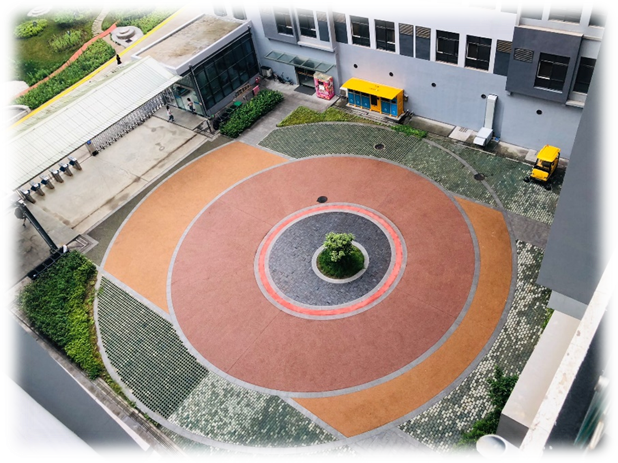
\includegraphics[width=0.8\linewidth]{pics/chp2_rainbow_dormitory}
	\end{figure}
	
	\hypertarget{ux6574ux4f53ux5916ux89c2}{%
		\subsubsection{整体外观}\label{ux6574ux4f53ux5916ux89c2}}
	
	彩虹楼面向外侧的楼上镶嵌着一些五颜六色的色块、彩虹色的线条,非常具有当代大设计家、艺术家的设计时尚。走进楼内,一种划时代的公寓气息扑面而来, 8座电梯,全楼层通达(虽然写着单双号)。
	
	\begin{figure}[htbp]
		\centering
		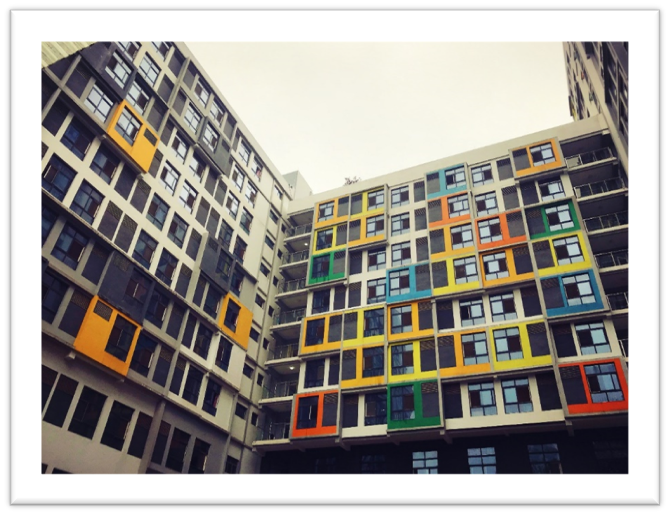
\includegraphics[width=0.6\linewidth]{pics/chp2_rainbow_outlook}
	\end{figure}
	
	\hypertarget{ux5185ux90e8ux7ed3ux6784}{%
		\subsubsection{特点和一些实用性建议}\label{ux5185ux90e8ux7ed3ux6784}}
	
	1.唯一的有电梯的女生寝室楼(划重点)。
	
	2.没有独立卫生间,有阳台(约15平方米),四人一间(约25平方米)。
	
	3.相差两个房号的寝室阳台相连(如711和709)。
	
	4.床,桌柜都较新,每个桌子都只有一个插座,注意自备插线板,建议购买台灯。
	
	5.不熄灯断电,走廊灯24h不灭。
	
	6.十一点半后关闭寝室大门,需晚归出行时记得带上门禁卡(校园卡)。
	
	7.床规格是 190cm$\times$90cm,推荐床帐蚊帐一体式全框架,半框架可能会比较麻烦,所以建议小伙伴选择 190cm 的床帐。
	
	8.空调可以用支持红外线遥控的手机开启,注意开空调的发票和清单要保存下来,不要弄丢,毕业时需要凭此退还押金。
	
	9.基础电费每月似乎 150 度,每学期均可找一楼宿管阿姨要对应宿舍的电卡,在门口的电箱中刷卡即可完成充值;建议在康桥一楼西侧提前购买。
	
	10.开学的时候可以选择在西十五租饮水机,会有人定期将饮用水桶搬运到对应的楼层,自行安装,比较方便。由于楼层水房还是只提供滚烫的热水,想及时喝到水温合适的水的同学建议入手饮水机。
	
	11.彩虹楼的四个网口一直有一个能用,但是由于插电问题,插线板还是相当有必要的。
	
	12.办网络套餐请浏览nethelp.xjtu.edu.cn。网络有问题请联系网管协会的同学。
	
	13.彩虹楼有单独澡堂,水量大、温度合适、空间大、女生专用,离宿舍近(对彩虹楼的女生来说)。
	
	\subsection{男生:西十四舍}
	
	\begin{figure}[!h]
		\centering
		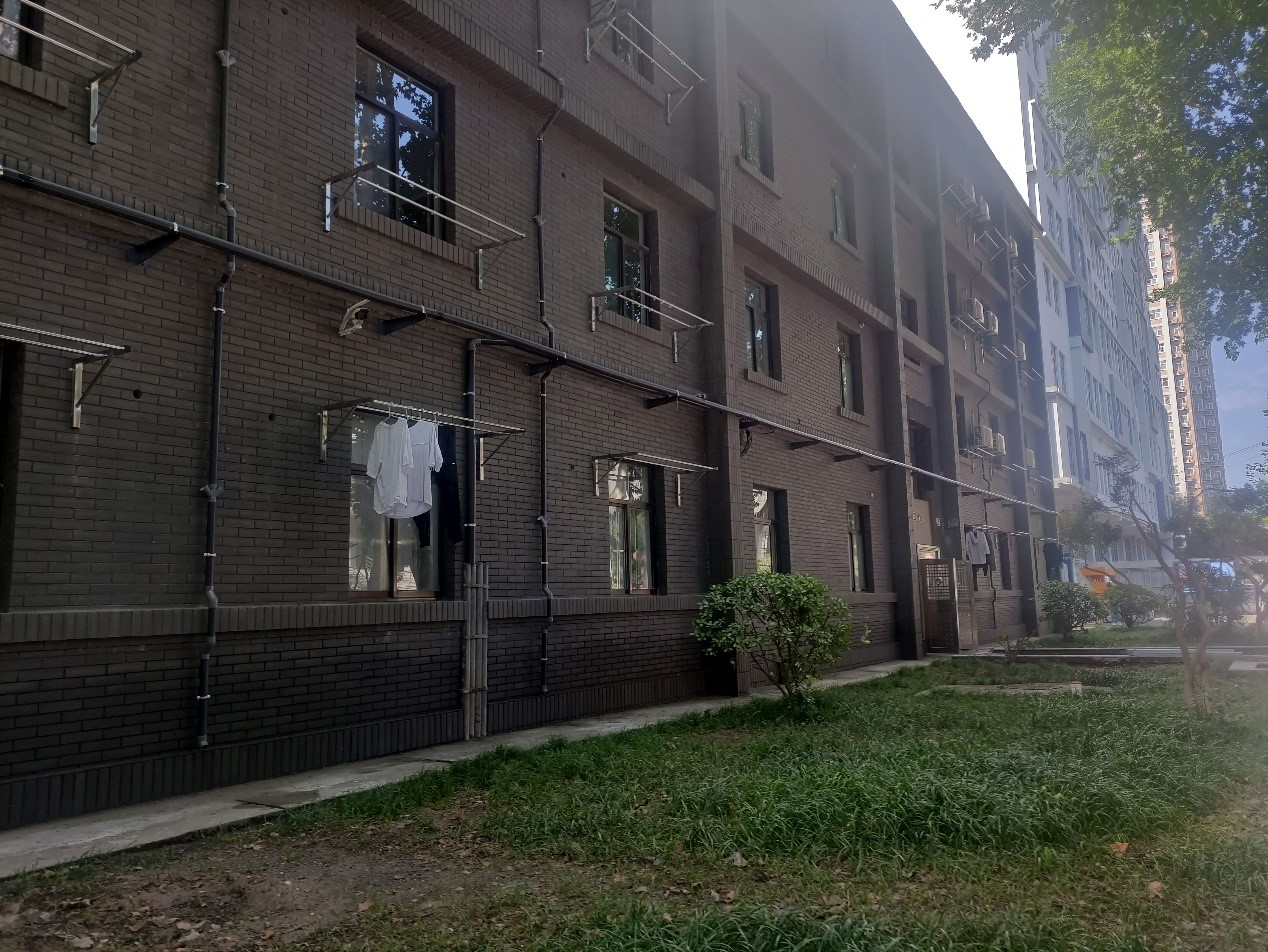
\includegraphics[width=0.8\linewidth]{pics/chp2_west10_dorm}
	\end{figure}
	
	\subsubsection{整体外观与外部环境}
	宿舍位于西南宿舍群中心地带,南侧紧邻快递街,取快递非常方便,但白天可能较为喧闹。北面于梧桐苑只隔着留学生公寓,饮食很方便。宿舍临近电动车充电桩(崇实书院和西十五之间,或彭康楼停车场旧水房背后皆有)。宿舍外观西迁风格保存较为良好,而内部是经过装修的,大家不用担心条件太差。
	
	\subsubsection{内部结构}
		
	西十四宿舍内部多为四人间寝室,四张床用ABCD编号,编号顺序是进门左手靠门的床位是A,俯视顺时针数,直到进门右手靠门的D床。AD床靠门,BC床靠窗。宿舍AD床与门的间隔之间有储物格,适合放置起居用品或者展示装饰品、手办等,进门头顶上也有面向窗户开口储物仓,可以放一些大件行李,放置、拿取的时候注意安全,可以借助AD床传递。

	\begin{figure}[!h]
		\centering
		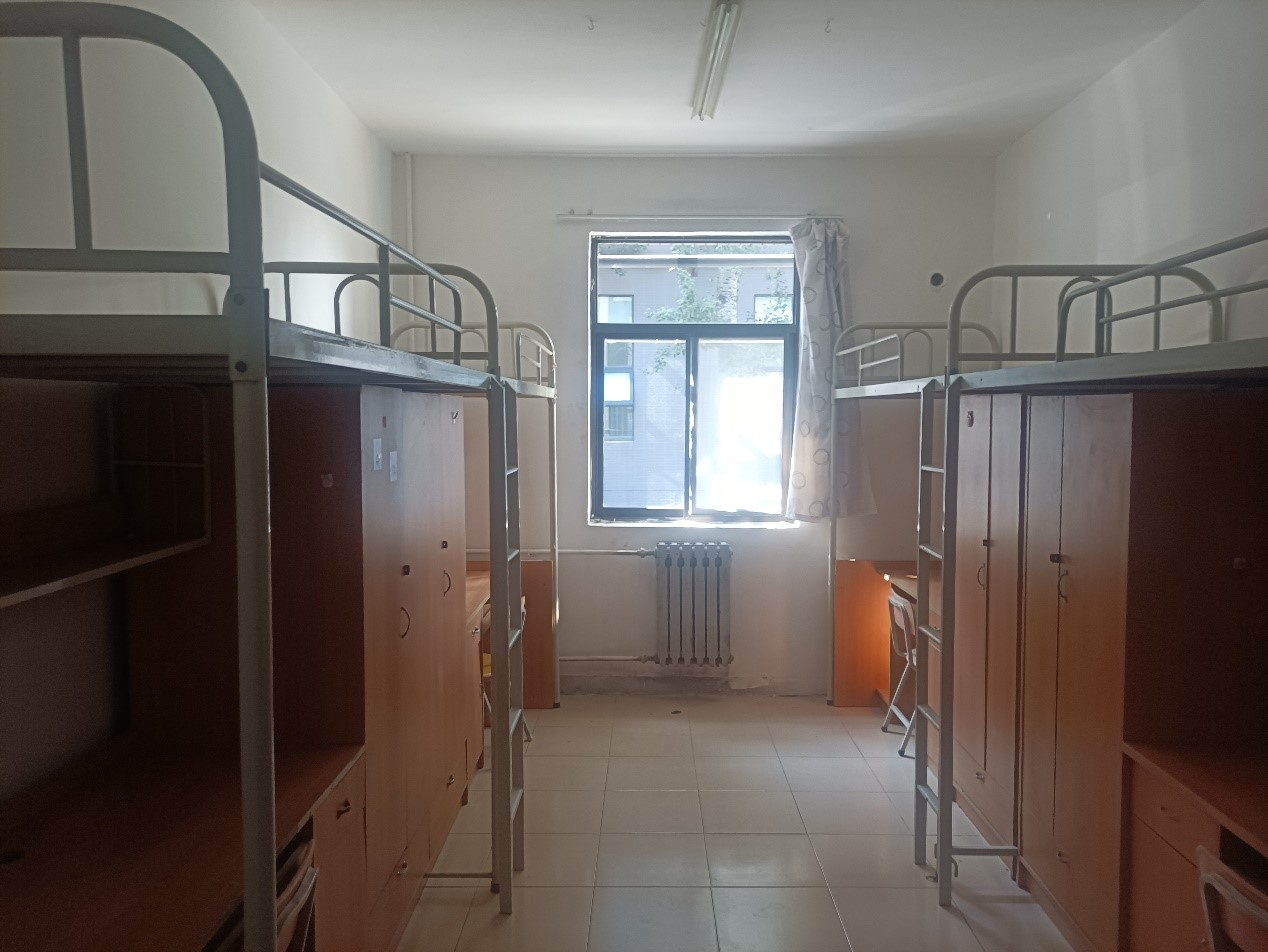
\includegraphics[width=0.8\linewidth]{pics/chp2_west10_dorm_inside}
	\end{figure}
	
	
	西十四宿舍中每个同学会分到独立的上床下桌,有键盘仓、机箱仓、走线孔等。衣柜上有锁位,锁具需要自备。衣柜内靠床尾向有小层,上部有晾衣横杆。
	
	桌上靠衣柜一侧有书柜,开口与人面向的方向垂直。书桌与墙面之间没有防桌上掉落的挡板,可以考虑自行加装。书桌配备的椅子为以前教室课桌的椅子,空间较为局促,建议想更换椅子的同学实地测量后再决定。
	
	床铺的尺寸为1.9m*0.9m,高度一般可以放下1.1m高的蚊帐,同样建议实地测量后再决定尺寸。寝室配备了空调,安装于窗户上,BC床可能容易着凉。
	
	暖气片在窗户下方,注意请不要在暖气片上或附近搁置易燃物品或烘干潮湿物品,容易糊。
	
	每位同学的桌子后都有一个标准插座可以取电,建议购买插线板延长、扩容后使用。还有四个网线插座,但一间寝室只有一个可用。由于装修费力,在上一次寝室的装修中一次性安装了四个插口。若一个网线口出故障,可以联系开启下一个插口使用,免去了需要重新改造线路的困难。为了避免寝室多人分散使用网线口造成故障分散累计,四个插口只开启一个。有需要的宿舍可以自行购买加装无线路由器和分线器等辅助日常网络使用。多次校园网升级改造后,网络的使用水准已经有了较大的提升,但不可避免在集中用网等时期仍会有卡顿、丢包等故障情况,请及时与网信中心联系修复故障。

	
	\begin{figure}[!h]
		\centering
		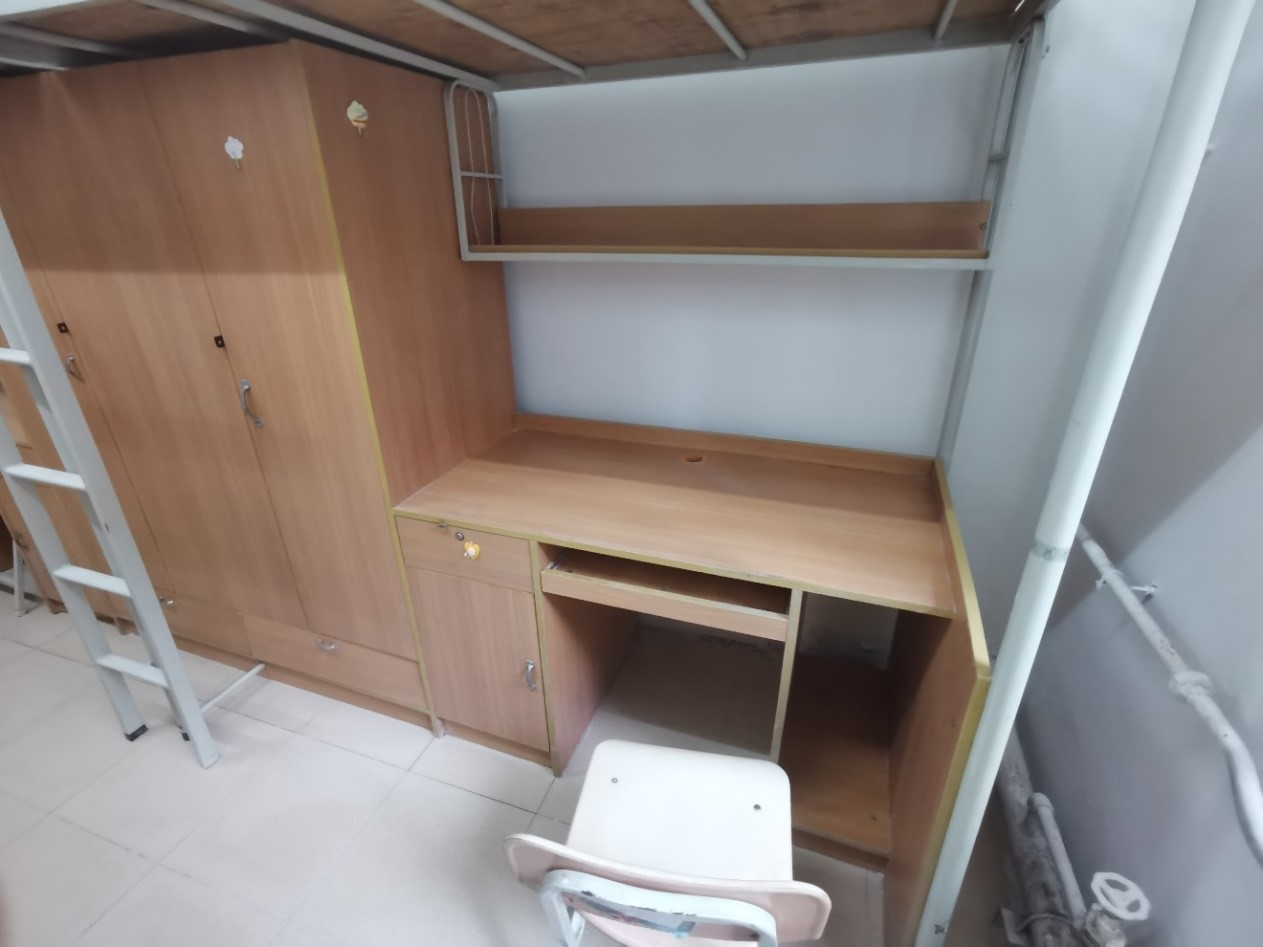
\includegraphics[width=0.8\linewidth]{pics/chp2_west14_dorm_desk}
	\end{figure}
	\vspace {-1.5em}
	\subsubsection{硬件条件}

	寝室的内外是两个装修风格,不要被古旧的外墙吓退了,内部的装修仍然是现代的。

	\begin{figure}[!h]
		\centering
		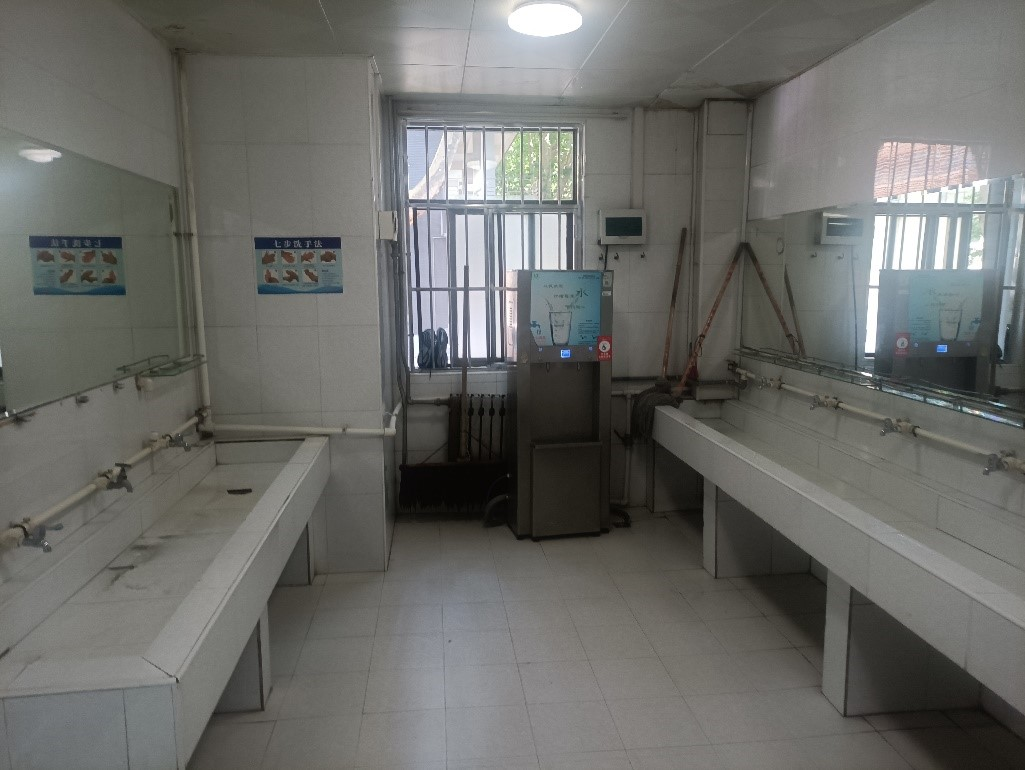
\includegraphics[width=0.8\linewidth]{pics/chp2_west10_dorm_wc}
	\end{figure}
	
	每层楼在东西两侧各有两个水房和卫生间,每日有保洁校工前来打扫。卫生间的水龙头只能出凉水。1楼设有洗衣房,可以下载对应的软件操作洗衣,价格较为便宜。每层楼有一个水房里有开水机,可以满足日常使用需要。
	
	窗外设有晾衣杆,不过由于后装的限位器的存在,使用可能会困难一些。走廊内也有晾衣绳,虽然是阴干的,但是由于气候较为干燥,衣服晾干一般不会太久。提醒各位同学在晾衣服前自己或找同学帮忙把衣服拧干,否则会一直滴水,影响过路的同学,还会有安全隐患。

	在2023年暑假里,西十四宿舍里修建了公共浴室,洗澡不一定需要前往外面的东区、崇实、文治等澡堂,更加方便喵。
	
	宿舍楼梯较陡而且部分楼梯不规则,上下楼梯请注意安全。

	请注意,不要将电动车电瓶带入楼内充电,不要在楼内吸烟,不要饲养宠物,谨慎使用大功率电器,不要使用电热毯、便携式烧水壶、加热棒等电器,注意水电安全和维护良好的起居环境。

	
	\subsubsection{水电缴费}
	最后是水电缴费问题。宿舍的供水问题是由水房解决的,如果需要水的话,一般取同层的水房打水就可以解决问题。每层的两个水房中,有一个安装了饮水器,可以提供热水。有需要的同学也可以在寝室内安装一台饮水机,同时向学校订购桶装水。
	
	每位本科生每个月都可以领取到11度的电,每年的3月、9月下发。电费计算是以寝室为单位的,也就是说每个寝室平均每个月有44度的免费电可以用。如果超过这个额度,就需要交电费了,可以前往康桥苑一楼西北角的购电窗口办理手续,预存或补交电费。电量用尽后会自动跳闸,建议定时在宿管阿姨处查看电量,观测用电习惯,节约用电。


\section{行}



\subsection{交通工具}
\subsubsection{共享单车}

学校内有哈\Noto{啰}单车(「小蓝车」)和美团单车(「小黄车」)两种共享单车,分别使用哈\Noto{啰}出行/支付宝和美团/微信进行租车。主要停放在东南门西侧、康桥苑西北侧、主B西侧、
梧桐苑东侧、
宿舍门口(集中在崇实和南洋外)等地点。


校外也有共享单车,可根据日常需要使用。其中,东南门外的共享单车停放地点在东南门门口和天桥东侧下面;西南门外的共享单车停放地点在西南足球场外侧,从西南门往南走即可。\textbf{(!\ !\ !)注意哈\Noto{啰}在校内的大部分单车为校园车,不要骑到校外,否则会扣20元调度费。}

注:下载哈\Noto{啰}出行APP,完成学生认证,有两个为时一周和一个月的学生优惠。此外,相关平台有单车会员和外卖等会员的联合会员。因学生会因课程经常需要在20分钟甚至更少的时间在主楼上课地点和中一、二、三等楼之间往返(不到800m),可按需购买。

\subsubsection{公交地铁}

兴庆校区各个校门外均有公交站,其中南门外叫做“交大南门”,东南门外叫做“沙坡村”,北门外叫做“兴庆公园南门”,西南门外叫做“兴庆西路建东街口”。故在后面交通路线叙述中,“xx门坐xxx路”默认指从上述公交站乘坐。

距学校最近的地铁站为交通大学·兴庆宫站,为六号线车站,可从北门出发向东行走50米抵达。

离学校较近的地铁站为雁翔路北口站和太乙路站,均为五号线车站,其中前者从南门或东南门走较方便,后者从西南门走较方便。如需乘坐其他线路,可在地铁线网内换乘,或步行及通过公交转乘,如东南门向东可步行至三号线延兴门站,南门外乘坐700路可到达四号线“建筑科技大学·李家村”站(下简称李家村站)及二号线南稍门站。

西安的大部分公交均为两元一票制的空调车。地铁按乘坐距离票价为2-14元不等,比如以雁翔路北口站为例,到大雁塔站只需2元,到西安北站(北客站地铁站)需5元,到创新港站需8元,到机场(机场西地铁站)需9元。平时乘车时可使用长安通公交卡,公交五折地铁九折。学校随通知书邮寄的学生卡就有长安通功能,但与平时食堂吃饭的余额是两个账户,长安通功能需单独充值,此外如饭卡丢失后长安通部分无法挂失,补办的饭卡也没有长安通功能。此外,西安公交地铁也支持扫码乘车,但需注意公交和地铁乘车码不同,公交与长安通实体卡一样可享受五折优惠,但地铁无折扣。此外,如有经常乘坐远距离地铁的需求(如去机场、创新港、兵马俑等地),可购买西安地铁次卡,会在每年年底及新线开通等重大时间点发行,发行后三年有效,目前发行价平均每次5元;该卡在闲鱼上也有售,但黄牛出售的价格比官方价格高。






\subsection{校内外的公共设施}


\subsubsection{医院}

\textbf{西京医院:}学校北门乘坐410/512路公交车,或学校东南门对面乘坐408、508、517等公交车,西京医院站下车。

\textbf{武警医院:}学校南门过天桥后直行500米,在南二环南侧。

\textbf{第九医院:}学校南门向西走到经九路路口,沿着经九路向南走至南二环入口,位于入口西侧。

\textbf{校医院:}位于学校东南门南侧,温泉浴室隔壁。

\subsubsection{邮局}

收取挂号信、印刷品、汇款单在北门邮政处,而邮政速递的快递包裹在西14和西15之间的快递街领取。学校内东南足球场和网球场之间、彭康书院附近有家邮局。可以寄国际国内各种邮件,包括明信片、挂号信、包裹等。平时如果有邮寄需求,一般邮政收费比其他快递公司低。此外,校外也有多家邮局,规模较大、营业时间较长的是钟楼邮政支局,可从东南门乘坐45或南门乘坐252及612至钟楼西站到达。

\subsubsection{银行}
学校内有工行网点(仲英书院楼下、卡务中心旁边)及中行和工行的ATM机多台(中行位于主A楼下,工行分布在工行网点旁、东七宿舍楼下、中二楼等多地)。此外,校外也有中行、工行、农行、建行、交行等多家银行网点。

\subsection{校外大商场}
\subsubsection{华润万家}

华润万家是一个大型超市,里面的东西(尤其是牛奶、水果等)比校内超市便宜,在一些时候还会有优惠券。在门店外还有一些小餐馆,如兴庆路店外有肯德基。

\textbf{位置:}兴庆路店:东南门过天桥向北;兴庆南路店:东南门过天桥向南。这两家店均离学校较近,步行即可。此外,西安市区其他位置也有不少门店。



\begin{figure}[htbp]
	\centering
	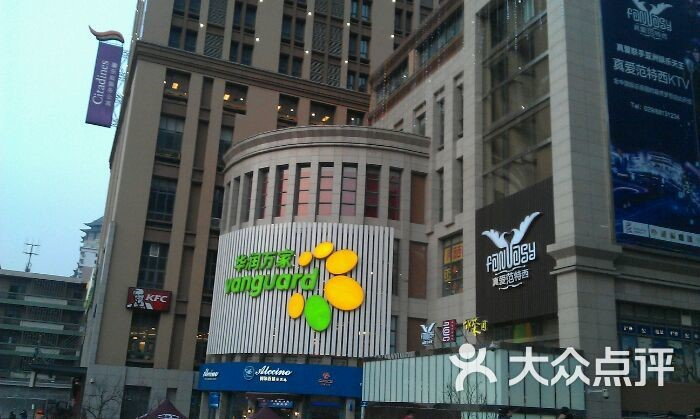
\includegraphics[width=0.8\linewidth]{pics/image19.jpg}
\end{figure}

\subsubsection{立丰国际购物广场}



\begin{figure}[htbp]
	\centering
	\includegraphics[width=0.8\linewidth]{pics/image20.jpg}
\end{figure}

\textbf{位置:}
位于交大三村东侧,东二环路上。可从东南门往东走,在延兴门地铁站附近往北边转,步行路程约1.2公里,18分钟。

\textbf{美食推荐}

多人聚餐

6F:潮汕牛肉锅、探鱼(烤鱼)、呷哺呷哺(火锅)、嗨捞猪肚鸡、奥赛奥章鱼水煎肉、九田家(韩式烤肉)、鑫海汇(自助)

7F:老重庆真味火锅、海底捞

8F:西安饭庄

奶茶小食

1F:蜜雪冰城、茶话弄、DQ、味千拉面、绝味鸭脖、快乐柠檬

2F:麦当劳、必胜客、星巴克

6F:茶话弄、书亦烧仙草、泰熙家(韩料)

\textbf{购物指南}

1F:沃尔玛

2F:屈臣氏

5F:Adidas、Nike、Fila、Puma、Kappa、Converse等

\textbf{其他}

9F:幸福蓝海影城、绿树网咖。

\subsubsection{万达广场(李家村店)}

\begin{figure}[htbp]
	\centering
	\includegraphics[width=0.8\linewidth]{pics/image21.jpg}
\end{figure}

\textbf{位置:}
位于李家村十字。可从南门坐700或313路或西南门坐49路到李家村站下车,也可乘坐五号线至李家村站。若步行,可从南门或西南门出来沿友谊路向西走,步行距离约两公里,时间约半小时。


\textbf{美食推荐}

多人聚餐

3F:呷哺呷哺、遇见长安、九锅一堂

4F:海底捞

奶茶小食

1F:哈根达斯、麦当劳、肯德基、一芳水果茶

2F:鲜芋仙、DQ

3F:茶话弄、COCO都可、比呐食手打虾滑、板戒排骨、味千拉面

\textbf{购物指南}

B1:沃尔玛

1F:屈臣氏、Adidas、Nike、Puma、H\&M、优衣库等

\textbf{其他}

4F:万达影城。

\subsubsection{赛格国际购物中心}


\begin{figure}[htbp]
	\centering
	\includegraphics[width=0.8\linewidth]{pics/image22.jpg}
\end{figure}

\textbf{位置:}
位于小寨十字。可从南门或东南门坐401至小寨站下车,也可乘坐地铁2、3号线到小寨地铁站(如从太乙路进站,在南稍门换二号线较方便;如从雁翔路北口进站,在青龙寺换三号线比较方便)。打车约15元,但周末高峰期可能堵车。

\textbf{美食推荐}
多人聚餐

6F:嗨捞猪肚鸡、遇见长安

7F:九锅一堂、呷哺呷哺

9F:海底捞火锅

奶茶小食

B2:鹿角巷、COCO都可、绝味鸭脖、文和友老长沙臭豆腐

1F:奈雪的茶、喜茶、星巴克

6F:卡米拉雷门拉面、瑞可爷爷的店、廖记棒棒鸡、快乐柠檬

7F:必胜客

\textbf{购物指南}
B2:名创优品、NOME

B1:VANS、Adidas、Nike、Puma、Dickies、Boy
London、NEWBALANCE、EVISU、Timberland、中国李宁、优衣库等

1F:屈臣氏

5F:Adidas、Nike、Puma、李宁、Fila、Kappa、asics等

\textbf{其他}
赛格的6-7F有很多的美食,也有很多大牌、潮牌的店,很适合逛街,不过要记得「量入为出,适度消费」!

此外,赛格周边也有一些商场,比如海港城、华旗国际广场等,有很多适合做手工DIY、美甲等的地方,也有一些适合小众爱好的地方,大家可以在各种APP上自行探索。

\subsubsection{西安大悦城}


\begin{figure}[htbp]
	\centering
	\includegraphics[width=0.8\linewidth]{pics/image23.jpg}
\end{figure}

\textbf{位置:}
位于大雁塔西侧,大雁塔广场内。可从东南门坐408路公交车,在「雁塔西路东口」站下车(但408路末班时间较早,为21:00,可能无法通过此方式返回学校)。也可乘坐地铁至大雁塔站(如从太乙路进站,在李家村换四号线较方便;如从雁翔路北口进站,在青龙寺换三号线比较方便)往南步行即可到达。从大悦城打车到学校约10元,走路约需一小时。

\textbf{美食推荐}

多人聚餐

3F:分米鸡、\Noto{湊湊}火锅茶憩、金牌泰香米、小吊梨汤

4F:胖哥俩肉蟹煲、薇酌饮、失重、starry、萤初炉端烧、绿茉莉、大渔铁板烧(自助)

奶茶小食

B1:拔戒排骨、小心虾滑、鹿角巷

1F:星巴克、喜茶、奈雪的茶、ZAKUZAKU

2F:爸爸糖手工吐司

3F:鲜芋仙


\textbf{购物指南}

B1:李宁、PUMA等

1F:Air Jordan、ZARA等

2F:优衣库、URBAN REVIVO、Bershka等


\textbf{其他}

大悦城也有很多好吃的、好玩的,以及电影院,而且一直都有免费展览,迄今为止已知有火影忍者、漫威等,是一个充满惊喜的地方!

同时,它在大雁塔和大唐不夜城附近,可以在购物、吃饭的同时欣赏大雁塔音乐喷泉和大唐不夜城的美景。比如在四楼就可以拍到很好看的照片!


\subsubsection{曲江创意谷}


\begin{figure}[htbp]
	\centering
	\includegraphics[width=0.8\linewidth]{pics/image24.jpg}
\end{figure}

\textbf{位置:}
位于曲江新区。可从东南门搭乘48路公交车,到「黄渠头村」站下车。

\textbf{美食推荐}

多人聚餐

仙麦精酿啤酒餐厅、海底捞火锅等

奶茶小食

茶话弄、奈雪的茶、爸爸糖手工吐司、泰熙家等

\textbf{购物指南}

O·C·E、优衣库、Adidas、Nike、Puma等


\textbf{其他}

曲江创意谷是一栋一栋的楼,很新潮的一个商圈,里面也有电影院,还有一些会出人意料的餐厅、小吃店和商店,很适合不带目的地逛逛。



\subsubsection{其他地点}
受篇幅所限,无法给出全部大商场地点,上述所列地点的推荐店铺也不完整。如此部分想获得更多更详细的信息,欢迎联系热心学长(西安本地人)计试001班赵宋文(QQ:791687308)。

\subsection{机场及火车站}
\subsubsection{西安咸阳国际机场}
咸阳机场离学校较远,可乘坐地铁到达(票价9元),约1.5小时,也可打车,约1小时,花费120-150元。%在西安咸阳国际机场可乘坐飞机到深圳宝安国际机场,约2.5小时,下机后可乘坐11号线至万象城,比上一节所述的大悦城、李家村万达、小寨赛格等都要好,还有很多比贾玉(20级钱班高数助教)好看的妹子。

\subsubsection{西安北站}
为高铁站,有18台34线,是全国目前站场规模最大的高铁站。
地铁较方便,有2、4、14号线,是目前线网内唯一一个三线换乘站。乘坐五号线至南稍门换乘二号线,也可乘坐六号线在大差市或钟楼站换乘二号线,约一小时。距离三个地铁站的距离视起始点而定,实际上没有什么本质的区别。

\subsubsection{西安站}
为普速车站,近期改造已完成,新站台、候车室已投入使用,乘车环境较好。

可以乘坐5号线在建筑科技大学·李家村转4号线,或者6号线在大差市转4号线前往,也可以出西南门向西走乘坐22路公交车到达。

\subsection{景点}
\subsubsection{华山}
位于西安东部的华阴市,从西安北站乘高铁,到华山北站后,有免费公交到达游客中心,1路或2路均可,下车后南行百米就是售票大厅。若想深度游览华山,可以尝试徒步,也可以选择乘坐西峰索道,居高俯瞰下面的万丈深渊。

\begin{figure}[htbp]
	\centering
	\includegraphics[width=0.8\linewidth]{pics/image25.jpg}
\end{figure}

\subsubsection{兵马俑、华清池}

\textbf{交通:}可乘坐地铁九号线到达秦陵西或华清池站转乘接驳车至兵马俑,票价8元(雁翔路北口——秦陵西)。也可乘坐游5路(306路),起点站在西安火车站东广场,终点站为兵马俑,中间会经过景点华清池,票价为阶梯票价,起步价2元,乘至兵马俑为7元,首班车:07:00;末班车:19:00

\textbf{门票:}建议提前在网上购买,到达景区时刷本人有效身份证即可进入,非常方便快捷。如需现场购买,一定在指定售票窗口或自助售票机上进行购买,避免上当。

\begin{figure}[htbp]
	\centering
	\includegraphics[width=0.8\linewidth]{pics/image26.jpg}
\end{figure}


\subsubsection{陕西历史博物馆:}

\textbf{交通:}东南门或南门乘坐401路公交车到陕西历史博物馆站下车即可。

\textbf{门票:}提前通过「陕西历史博物馆票务系统微信公众号」进行门票预约。

发售时间:

冬季:上午:09:00-\/-12:00

下午:12:30-\/-16:00

(11月15日-次年03月14日)

夏季:上午:08:30-\/-12:00

下午:12:30-\/-16:30

(03月15日-11月14日)

开馆时间:

冬季:09:00 停票时间:16:00 闭馆时间:17:30

夏季:08:30 停票时间:16:30 闭馆时间:18:00

周一闭馆。遇法定节假日周一正常开放。除夕闭馆。

\begin{figure}[htbp]
	\centering
	\includegraphics[width=0.8\linewidth]{pics/image27.jpg}
\end{figure}

\subsubsection{青龙寺}

春季四月为赏樱最好时期。可从东南门乘坐517路/48路/45路至青龙寺站下车,也可步行抵达。

\begin{figure}[htbp]
	\centering
	\includegraphics[width=0.65\linewidth]{pics/image28.jpg}
\end{figure}

\subsubsection{西安城墙}

西安城墙是一个完整的环,可以在上面骑自行车。有多个门可以进入,但最出名的门是南门(永宁门),离学校也较方便,此外,南门外还有西安SKP等多个商场,较繁华,故建议选择南门进入城墙。从学校去南门可乘坐五号线至南稍门站换乘二号线到永宁门站下车;也可从学校北门乘坐910/800/402/512路,至南门外站下车,后步行约700米。


\begin{figure}[htbp]
	\centering
	\includegraphics[width=0.7\linewidth]{pics/image29.jpg}
\end{figure}

\section{玩}
\subsection{运动健身}
\paragraph{足球}
东南足球场有三块五人制场地,一块十一人制场地,除此以外还有零星草皮可供使用。

西南足球场为一块缩小版的十一人制场地,使用率较低,周末会有初中生。

校外人员较多,注意财物与自身安全的保护。

\paragraph{篮球}
东南足球场西侧有两块篮球场,西南篮球场场地较大。

\paragraph{羽毛球、乒乓球}
交大的文体中心位于学校的西南门附近,内有各类运动场地。进入文体中心需要带一双干净的鞋进去换,刷一卡通进门。

乒乓球场地很多,需要提前预约,2元/桌,不限时间,直接在一楼扫码换鞋即可。不预约可能会被大妈赶走。

羽毛球场地较多,但是经常是爆满,尤其是晚上,需要提前预定,10元/桌,限时一小时。不预约可能会被大妈赶走。

其他场地:东南足球场东侧有石制的乒乓球台。

在康桥往主D的路上有两片羽毛球场地,水泥地。

\paragraph{网球}
交大有大量的网球场,分别分布在东南门门口(能动学院西侧)、东南足球场东侧、文体中心东侧、东南足球场南侧。

\paragraph{游泳}
交大游泳馆在能动学院北侧(东南门附近)。泳池为标准50m泳池。深水区水深1.8m,浅水区水深1.4米。

平时人较少,周末和暑假人较多。游泳馆白天并不对外开放,因为有游泳课,因此只有晚上可以去游。

年卡:300元/30次

单次:15元/次(带学生卡,可抵押钥匙)


\paragraph{台球}

交大校内没有台球厅。南门外有一个星钻台球俱乐部(只有8球),下午两点半开门,可以组团打麻将。晚上人可能会比较多。李家村附近有一家行者桌球(高德地图能查到具体位置)。

\paragraph{健身}

文体中心内有健身房,宽敞。设备不是很齐全,但对于一般的同学来说已经足够。一次2元。

校外有很多健身房,比如沃菲特、韦恩,可根据个人需要选择。


\subsection{社团、各种学生活动}

交大有很多社团,开学时会进行招新,可以根据个人兴趣和时间安排自愿加入。刚刚入学时会有学校和各个书院举办的新生篮球赛、足球赛、辩论赛等,此外还有各个书院的迎新晚会。平时学校也会举办很多比赛,如交大之星、交大演说家等。各个活动经常通过宿舍楼下张贴海报、食堂门口发传单或摆摊等方式宣传。

钱学森书院学生会开展的精品活动详见介绍篇。

\section{网络}
网络故障请在移动交大app(下面会介绍)内报修,欢迎有志向为宿舍网保驾护航的同学加入西交网管协会。群号:882622842

交大目前运营的网络有教育网(俗称校园网)和运营商网络移动、联通和电信供同学选择使用,满足同学们多元化的需求。

目前教育网和移动、联通、电信均可使用路由器,但不推荐宿舍共用一个网络。

入校后需要办理校园网入网,缴纳100元入网费,可直接使用教育网。办理移动、联通和电信套餐也必须在缴纳入网费后才可办理。


\subsection{宿舍网络}
\noindent \textbf{教育网}\\
优点:基本免费、资源丰富\\
缺点:流量有限、网速较慢、高峰期网速不稳定\\
带宽:教育网的带宽为30Mbps\\
资费:为每个月15G免费流量,15-40GB按1元/GB,40-50GB按2元/GB计算,超过50GB目前不计费。\\
\textbf{移动、联通、电信套餐}\\
可在WebNet服务中心的公众号了解详情,并购买。有价位不同的套餐可供选择。
优点:网速稳定、不限流量\\
缺点:固定费用、对部分游戏国外服务器不友好

\subsection{校园无线}
\noindent xjtulib\\
在图书馆可以使用免费无线,覆盖钱学森图书馆范围,入网后即可免费使用。\\
使用方法\\
连接xjtulib无线后,在弹出的网页中登录,帐号为NetID@xjtulib(NetID即为学生学号), 密码为校园网密码。连接上限为三个设备。\\
xjtu\_stu\\
在全校范围(主要覆盖:教室、图书馆、办公楼、学校主干道、食堂,宿舍区未覆盖)可连,入网后即可免费使用。\\
使用方法\\
连接无线网络后,在弹出的页面中登录(若弹出较慢,可以尝试输入地址10.6.18.2(适用主楼、中楼等区域)或10.6.21.2(适用于食堂、仲英楼等区域)强攻),账号为<学号>@stu,密码为校园网密码。\\
连接上限为一个设备,尝试登录多个设备会弹出“无响应数据“或空白窗口。由于自动下线时间约为5-10分钟,在切换设备用网时,建议在登录设备上回到登录页面点击”注销“,否则新设备会很长时间无法登入。\\
xjtu\_1x和xjtu\_wlan\\
仅供交大教职员工、维护人员和学生网络管理协会使用。\\
STU\\
在生活区,即宿舍范围覆盖。\\
连接无线网络后,在弹出的页面内登录(若弹出较慢,可以尝试输入地址10.6.11.8登录)账号为<学号>,密码为校园网密码。\\
连接设备数为2-3个,上限视购买套餐而定,若超过上限会转到已在线设备的ip地址页面,可以将已在线设备强行退出在线。有多设备登陆需求的同学可以记下设备的ip地址,或购买无线路由器。\\
xjtu\_JSQD\\
教室签到的入口WiFi,需结合移动交大app里的“教室人脸签到“功能使用,可以实现人脸签到。在教室打卡机、班牌刷脸异常拥挤或出现故障时可作为保险方案。该WiFi不连入互联网,不需要登录。\\


\subsection{入网申请教程}
\begin{enumerate}
	\item 登录 nethelp.xjtu.edu.cn
	\item 学生网络——>校园网申请:按照提示,申请,缴费100元入网费后开通
	\item 学生网络——>校园网账号信息:这里可以看到帐号密码信息
	\item 帐号为NetID,密码默认是随机6位数字,可以自行更改
	\item 校园网密码和NetID密码是分开的,在登录校园无线和移动联通帐号时使用的是校园网密码
	\item 在auth.xjtu.edu.cn(需要用校园网访问)可以查流量使用情况和改密码
\end{enumerate}

\subsection{移动、联通套餐}
\noindent 运营商网络套餐可供对流量和网速有需求的同学办理。\\
套餐办理也是在nethelp.xjtu.edu.cn\\
选择“学生网络”→“选择套餐”→“套餐办理”

\subsection{宿舍网络使用}
\noindent 每个宿舍只有一个有用的网线端口!\\
其余的均为备用,防止网线在墙体断了,更换麻烦。\\
一般有用的网线端口为靠门两张桌子下面的一个。


\chapter{学习篇}
\section{校园常用网站一览}
\subsection{教务处}
\url{http://dean.xjtu.edu.cn}

将dean换为jwc、due也可以登入,或直接搜索西安交通大学教务处。教务处首页会展示有关于科研学习的最新公告,通过右下角的快捷通道则可以直接进入“综合教学服务平台”、“选课端”和“思源学堂”等,均需通过已有的 net ID(迎新时应已在移动交大 APP 上注册)进行登录。

\subsection{综合教学服务平台(ehall) 西安交通大学教务办事服务大厅}
\url{http://ehall.xjtu.edu.cn}

该平台主要用于各类教学活动的个人信息整理发布,包括个人的课表、考试安排、培养方案、转专业和成绩查询等。平台上有很多有用的信,因此经常关注该平台对于有效处理好大学学习是非常重要的。

\subsection{选课端}
\url{http://xkfw.xjtu.edu.cn/}

该平台只用于选课,相关的选课信息和选课类型(预选或即选即得)会提前发布在教务处首页,选课前需及时关注公告,最好按照建议的选课顺序进行选课。预选,即报名可超过课容量上限,该轮结束后系统随机抽出中选的同学;即选即得阶段需要“抢课”,只要有空余容量即可选中课程。

\subsection{思源学堂}
\url{http://syxt.xjtu.edu.cn/}

思源学堂中有许多开放课程的教学视频,可以在此进行拓展学习。点击思源学堂后在新页面中点击用户登录,即可进入思源学堂(bb平台)。思源学堂是学生线上提交作业的主要平台,也是查看线上成绩、了解课程大纲、收到课程通知以及教学进度的平台,一些课程群(qq群或者微信群)的二维码也会放在此处,需要注意即时查看。

\subsection{Black Board平台(简称BB平台)}
\url{https://bb.xjtu.edu.cn/}

老师和助教会将学习资源(ppt 和讲义等)、课程公告、作业的布置、提交和批改、公布考试分数等教学内容统一通过该平台发布。该平台主要用于教学日常活动。进入思源学堂后,可以看到最新的公告和右侧的课程列表,点击右上角的个人信息旁小箭头可拉出菜单,可访问最新的未读消息和最新的评分等。通过该平台可以下载学习资源、在线学习、提交作业等。 

\subsection{畅课平台}
\url{http://class.xjtu.edu.cn/user/courses}

在BB平台中点击右上角“课堂视频“就可进入录播平台,平常教室里上的课可以在这里找到录像。有些教室的设备可能不太好用,音画质量出入较大。

\subsection{图书馆}
\url{http://www.lib.xjtu.edu.cn/}

图书馆网站的功能非常多,如查找纸质图书存放位置、索引文献网站如CNKI等、预约座位、预约图书馆讨论空间等。部分功能限制使用校园网,可以使用webVPN登录。

\subsection{师生综合服务大厅}
\url{http://one2020.xjtu.edu.cn/}

这里主要会办理寒暑假的请假销假手续。请销假一般只是走个流程。校外机动车入校等服务也是这里登记。

\subsection{西交webVPN门户}
\url{https://webvpn.xjtu.edu.cn/}

可以在校园网的相关说明上找到这个网站。这个网站是用于浏览器访问校园网访问的内容的,例如登录图书馆预约座位、空间,查询考勤状态等。与SSLVPN相比更加便于操作。

\subsection{西交办公自动化平台}
\url{http://oa.xjtu.edu.cn/}

这里会发布一些关于办公的通知。多数通知和我们并无太大关系,但是部分后勤通知如停水停电、供暖停暖、节庆日加餐券会在这里发布消息。

\subsection{综合信息服务平台}
\url{https://info.xjtu.edu.cn/}

正如它的名字,这里什么信息都有,交大几乎所有信息都在这里,但是也很没有重点,使用不多。

\subsection{学生工作管理信息系统}
\url{http://nsa.xjtu.edu.cn/}

这里主要是发布奖学金相关信息的,很多功能没有启用。

\section{教材购置指南}
教材的购买主要有三种方式:(1)统一购买;(2)自行购买;(3)网络购买。

\subsection{统一购买}
在学校相关链接或指定地点上交完书费后,可凭借收据或线上支付截图(可能存在少量没货的现象)。 因为通过该方式订书的人少,同时教材科前几天只对统一上交书费的同学服务,所以这种方式可以一次把大部分教材拿齐,且免去了后期繁杂的排队过程;缺点是其中包含了许多可能不需要专门购买的教材,买书的费用要明显多的多,学期末还有多退少补的过程。

\subsection{自行购买}
自行购买最常用的是教材科购买或购买旧书。

教材科位于东南门靠近仲英书院处。购买出版书籍打九折,未出版书籍只收取工本费,相比于上交书费,可有目的地只购买一部分学科的教材;缺点在于通过该方法买书的同学较多、排队时间较长(峰值可达到30min左右)、寻找教材过程较为困难(尤其需要注意区分英语书的学生用书和老师用书),此外也有可能遇到缺货的情况。但由于其方法既可以灵活购买,又可以及时买到新教材,因而仍然是大批同学的第一选择。

学校内较大的旧书店是阿善旧书,位于康桥三楼。其同时提供了专业组合套装书和单本书的同时售卖,售价大约为定价的一半,其专业组合套装书严格按照专业书单配置,因此也包括一些可能不太需要购买的书籍。需要注意的是,教材经常会更新换代,不光老师会按照新版本教材布置作业,实际学习体验中新版教材也较好,如《工科数学分析》第三版排版清晰度好于第二版,《大学物理》新版彩印版比《大学物理学》黑白版阅读体验更好,知识重点更加清晰,因此尽量购买新版是有必要的,在购买旧书前应关注版本问题。

\subsection{网络购书}
除上述两种方法外,网络购书也是一种方法。但是交大的部分教材为自行编写出版,网络上不一定有售卖。网络平台很多,鱼龙混杂,质量不一定有保障。笔者推荐去孔夫子旧书网购买,在上面买了一半的教材,一般没有劣质的书籍,很多时候一本品相像话的书算上快递只需要几块钱。但是,购买旧书需要一定经验,请务必谨慎购买,防止财产损失。

\section{课程简介}
\textbf{说明:}以下课程安排及相关试验班介绍按照历届情况编写,请同学们以个人培养方案为准,以下仅作参考。关于各专业的课程安排和培养方案,请前往\url{ehall.xjtu.edu.cn}登录查询。获取学习、备考资料,请加钱院学辅交流分享群。
。

\subsection{基础课程简介}
\paragraph{(1)高等数学}
\subparagraph{课程要点}
本课程又称工科数学分析基础,是大学最重要的一门基础课,是后续一系列课程的学习前提。高等数学主要介绍极限、一元函数的微积分、无穷级数、多元函数的微积分、场论、微分方程解法。

\subparagraph{学习技巧}
高数平时的学习分为线上和线下两个部分,线下是老师课堂的授课以及课后作业,线上则是MOOC的学习和网上习题。

\paragraph{(2)线性代数}
\subparagraph{课程要点}
本课程主要介绍行列式、矩阵等一系列数学工具,是以后课程的重要基础。

\subparagraph{学习技巧}
线性代数的难点在于全新的概念,入门时期的授课至关重要。建议认真看书;除做题之外,还需要摸透课本的思想和方法。难度较高等数学略低。

\paragraph{(3)大学英语}
本课程平时成绩占比较高。

除了基础的英语课程之外,决定或考虑出国的同学们需要尽早准备托福、雅思考试,以免影响申请出国交流项目。

\paragraph{(4)思政课}
本课程包括思修、毛概、近代史,类似中学的文科科目。大部分课程需要撰写论文,小部分课程需要按时完成网课任务————网课也有一部分成绩占比。

\paragraph{(5)大学计算机基础(程序设计)}
\subparagraph{课程要点}
本课程主要内容是计算机的结构、原理,基础知识、C语言及编程。作业为C语言的练习题,每一周大约8-12道。

注:计算机试验班的此课程以【计算机程序设计】代替。参照计试相应条文。

物理试验班此课程教授内容为【Python】而非【C语言】。参考物试相应条文。

\subparagraph{学习技巧}
本课程分为理论和编程两部分。理论部分考试以选择为主,建议认真听讲、把握重点。针对编程,要重视上机和作业,不论是python还是C/C++都需要自己多尝试、多做,培养一定的编程思想。考试难度中等。

\paragraph{(6)大学物理}
\subparagraph{课程要点}
大一下学期主要学习力学、电磁学和狭义相对论,较为基础,考核分为两次阶段测试和一次期末考试。阶段1考察力学、阶段2考察电学和狭义相对论,期末考试则是全面考察。大二主要学习热力学、波和光学。物理需要高等数学基础。

\subparagraph{学习技巧}
认真阅读课本、仔细完成作业、掌握课后习题、及时复习总结。

\paragraph{(7)大物实验}
\subparagraph{课程要点}
本课程是以大物理论知识为基础进行的实验操作。按照要求预习,实验前仔细听实验操作过程讲解。

\subparagraph{课程内容}
大一下学期的第2周开始,做12次课上实验和一个电脑端仿真实验;实验报告要求记录原始数据和计算处理数据;总成绩为每一次实验的成绩之和。部分班级可能有期末考试,考试内容为现场做实验、记录数据。

\subparagraph{学习技巧}
实验之前认真预习,写好预习报告。严谨实验,客观记录数据,生成实验报告。撰写实验报告熟能生巧。

\paragraph{(8)大学化学(钱学森班上的课为化学原理)}
\subparagraph{课程要点}
本课程重点在于物质结构、化学热力学、化学平衡等方面,相当一部分内容源于高中选修4。内容较杂、较广、较浅。\\
钱班的化学原理课程涵盖无机和有机部分,无机内容有原子结构、分子结构、宏观物质及其聚集状态、化学热力学平衡、化学反应平衡、水溶液中的平衡、电化学基础、化学反应速率。有机部分的内容有烷烃、烯烃、炔烃和二烯烃、脂环烃、芳烃、多环芳烃和非苯芳烃、立体化学、卤代烃、醇和醚、酚和醌。同时这门课也包含了化学实验课。

\subparagraph{课程考核}
会布置课后习题。考核方式为期中和期末考试。\\
钱班的化学原理课程有半期和期末考试。开学至半期由张志成老师上完无机部分,半期到期末由王婉琴老师上完有机部分。半期只考无机,期末只考有机。如果缓考或者补考,则需要将有机和无机合在一起考,难度较大。无机部分会有纳入考核的日常作业,有机部分老师不强调检查作业,建议结合自身掌握情况完成。

\subparagraph{学习技巧}
重要公式需要理解、运用。多阅读课本,注意细节。\\
钱班的化学原理课程节奏非常紧,老师没有太多时间带着复习一遍拉线索,所以平常就保质保量完成学习任务非常重要。由于这门课只有钱班在上,故往年题很难找,不过题都是任课老师出的,平常可以注意一下老师明示或暗示的重点。

\subsection{越杰班}\subsubsection{寄语}
首先恭喜学弟学妹们考入越杰班,你们将拥有最优质的资源与最光明的未来。

但学长学姐要提醒大家的是:进入越杰班并不意味着进入保险箱,更不能觉得自己很了不起,任何时候都要以谦卑的姿态踏踏实实地努力。上大学后没有父母老师的监管,你的生活完全由你做主。有的人努力学习了一年,有的人打游戏打了一年,有的人社团活动参加了一年。不同人有不同的生活方式,但你一定要清楚自己的定位是什么,想要成为什么样的人。任何时候没有绝对的对与错,但你必须为自己的决定、行为负责。你的未来始终掌握在你自己手中。

最后说一下分流的事,算是给大家打一下预防针。越杰班有严格的淘汰机制,凡是存在挂科的均要分流,分流按照学年结算,即大一上挂科在下半学期各方面与其他同学一致,但升大二进入原专业的普通班级。

虽然大学对成绩要求远不及中学,但请大家务必重视每一次考试,尤其是高数这样挂科率较高的学科一定要好好学。另外希望大家对自己有严要求。申请国外大学时要看你的GPA(平均成绩绩点),所以不要把六七十分作为你的终极目标,任何时候,成绩是硬道理。

\subsubsection{特色课程介绍}
\textbf{大一上:}

【混班教学】数学类课程及化学实验与大类混班上课,大学化学、思想道德修养与钱院其他班级或ACCA混班上课;

【独立设课】为越杰班独立设课“通用学术英语”;

【优势所在】大一上可参加四级考试。

温馨提示:工程力学提前学军事理论和机械制图,但不学大学化学;电气提前学军事理论。

\textbf{大一下:}

【表达与交流】越杰班必修。这门课的重点是科技论文写作、演讲报告、电子邮箱求职信等。作业量较大,任务多,但过程也很有趣。课程考核为三次作业:一篇3000字以上的科技论文写作(需自行选题并调研),一份小组演讲作业(自行选题),一份电子邮件的修改。

【出国访学准备】越杰班必修。学习查阅英文文献,学习撰写英文论文主要训练综述,课堂上组织小组合作研讨,训练英文演讲报告。这门课的作业量极大,包括但不限于以下内容:每周一次的20min以上英语演讲听力并提交笔记,以及每周的论文阅读;自行寻找6篇以上特定主题的论文,阅读结束后写一篇2000词以上的文献综述;观看一部经典电影并制作海报,根据海报完成一次10分钟以上的有关电影背后文化的演讲;随机组队完成各种小组作业,例如讲解中国文化,学习论文中常见错误等等,每次小组作业均需要全组人进行presentation。据不完全统计,这门课的作业量大约是高数的2倍,大学物理的3-4倍,请同学们一定要合理规划时间,以免赶ddl赶到心累。

【制图】此门课程根据专业的不同分为两个难度:工程制图和机械制图。机械制图相对难一些,要求的内容比工程制图更多。此门课程主要考察空间想象能力以及作图能力。建议多动手画图,在实践中学习,做好平时作业。

【国防教育】此门课程主要介绍军事相关内容。老师课上会画重点,每学期的重点都不一样,期末题从画的重点里出。

\textbf{特别提醒:}

1.思想道德修养最好开学就开始背诵工作,边学边背,切忌积压到期末,其余学期的政治类课程同理。

2.对网课引起重视,尤其特别关注定期测试题以及相关课程要求(如课程讨论以及视频观看量)。该部分成绩在期末占较高比重。

3.英语类课程强调实践,对基础知识(单词、语法、听说读写)的练习讲解在频率和强度上远不及高中,需要大家特别关注,自己额外安排时间练习。

4.选修课每学期最多选两个,核心课每学期最多选一个,不推荐大一上选满课,匀出时间尽快适应大学生活节奏,尤其是争取在大一获得3.7+的绩点(因为只有这个时候课最简单,最容易刷绩点)。

5.2023级电类可能将不再学习工程制图和大学化学。

\subsubsection{出国项目及英语方面准备工作}
按照培养计划,越杰班同学在大三均要出国交流,对英语要求很高,所以在大一就要有所准备。

首先,越杰班要求在大一通过四级与六级考试;

其次,托福考试。按照越杰班的要求,如果要进入美国top30学校,托福成绩至少102分。

越杰班同学在大一即可修完英语6学分,同时需要在入学次年的10月份之前参加一次托福考试,为后续奖学金评选做准备。

\subsubsection{奖学金评选说明}
进入越杰班的同学在未挂科淘汰的基础上,均可获得6万元的基础奖学金,基础奖学金按月发放,即在校10个月每个月可获得1500元的奖学金。出国奖学金在大二上学期评定,主要评选依据是学分成绩和学科竞赛。有5\%的同学可以拿到36万的国际交流奖学金,有80\%的同学可以拿到18万,有15\%的同学拿到3万。

\subsection{钱学森班}
\paragraph{工程图学(3学分)}
\subparagraph{学时安排}
52课内学时 + 24课外学时(1-16周,后8周有两节课)

\subparagraph{指定教材}
\begin{enumerate}
	\item 《画法几何及机械制图》唐克中等主编,高等教育出版社,2017.4,ISBN 978-7-04-047329-2
	\item 《画法几何及机械制图习题集》许睦旬等主编,高教出版社出版,2017.3,ISBN 978-7-04-047330-8
\end{enumerate}

有的班用的是以下两本
\begin{enumerate}
	\item 《三维建模与工程制图》续丹、许睦旬主编,机械工业出版社,2020.8,ISBN 978-7-11-165652-4
	\item 《三维建模与工程制图习题集》续丹,许睦旬主编,机械工业出版社,2020.8 ISBN 978-7-11-165653-1
\end{enumerate}

\subparagraph{课程简介}
本课程主要教授工程图的画法,以及由此引申出来的一些机械结构的简答概述,主要培养严谨的思维和空间想象能力,对于学习机械能动等机类专业的同学们比较重要,需要认真听讲做笔记等。此外课程还将教授Inventor和AutoCAD的使用,这两个软件的使用也是日后较为重要的技能。
\par\setlength\parindent{2em} 课程作业量较为适中,在认真完成的前提下,一般一周需要2-3小时完成作业,助教老师会认真批改。考试难度与个人感受有关,笔者在此无法给出统一的概述。

\subparagraph{分数组成}
20\%期中+50\%期末+10\%平时作业+20\%答辩大作业

\subparagraph{考试题型}
补全视图,根据两个视图画出第三个视图,标注尺寸,少许填空题,总共5-8道大题。

\subparagraph{学习经验心得与经验分享}
\begin{enumerate}
	\item 平时上课尽量认真听讲,老师讲课对于理解课本内容的帮助很大,一定抓住。最好课前通读两本教材的相关内容,以免上课老师提到某点知识时因为找不到手足无措。
	\item 大作业内容是以小组为单位对给定的实体零件建模并答辩。大作业组队要合理,团队成员不能人人偷懒,应该在这个过程中学习相关软件的使用。同时也要有掌握相应的技术的同学,这样才能取得较好效果。
	\item 考前仔细看书,尤其重视书上的基本模型,例题和作业题。推荐大概浏览一下慕课课件,选做部分习题,仔细研究慕课模拟题。准备考试不在于试题数量,在于对试题的理解。由于考试安排等原因,一般复习所用时间在两到三天。此外,不必购买学解编撰的资料,不对标我校考试的实际,容易带来误导。
	\item 平时注重该课程的学习。工图是一门“手艺”,只有平时认真思考、完成作业,考试时才能做到面面俱到,拿到高分,否则,可能会错误百出。
\end{enumerate}

\subparagraph{课程重难点知识}
\begin{itemize}
	\item 所有与尺寸相关的内容(标准严格,容易漏错)
	\item 组合体三视图,尤其截交线,相贯线两个部分,考试重点。
	\item 剖视图,留意其与截交线相贯线的综合。
	\item 零件的常见结构工艺、结构、视图与尺寸,分类归纳书上的图样,记住其要点。
	\item 螺纹连接,记住图样和尺寸比例。
\end{itemize}

\subparagraph{推荐参考资料}
\begin{itemize}
	\item 《工程制图解读》中国大学MOOC平台 西安交通大学 续丹等:慕课平台
\end{itemize}

\paragraph{国防教育(2学分)}
\subparagraph{学时安排}
32课内学时(1-16周)

\subparagraph{指定教材}
\begin{enumerate}
	\item 《军事理论教程》,问鸿滨主编,西安交通大学出版社出版,2019.7,ISBN 978-7-56-931180-8
\end{enumerate}

\subparagraph{课程简介}
本课程介绍了国家安全,国防概况,军事思想,现代战争,信息化装备等内容。本课程属于思政类课程,在学习过程中只要认真学习就可以得到一个还不错的成绩。讲课时,老师会结合当下国际政治军事热点,趣味性较强,容易吸引同学注意。此外课程考勤较为严格,有固定座位,翘课是基本不可能的。

\subparagraph{分数组成}
60\%期末+20\%平时作业(50\%思源学堂作业+50\%汇报展示)+20\%线上慕课

\subparagraph{考试题型}
工程图学的考试题组成为:10*选择题+填空题+5*概念解释题+3*解答题/开放性问题。

\subparagraph{学习经验心得与经验分享}
\begin{enumerate}
	\item 老师讲授的内容就是考试的范围,认真听课一定会有收获。但是平时课程也可以不必过度关注,正常出勤以及完成作业即可。关注一下考勤,作业和展示即可。
	\item 大作业内容是以小组为单位对给定的实体零件建模并答辩。大作业组队要合理,团队成员不能人人偷懒,应该在这个过程中学习相关软件的使用。同时也要有掌握相应的技术的同学,这样才能取得较好效果。
	\item 考前约一周根据提纲看书,比较各种提纲和书的出入,确定要记忆的内容。
	\item 考前最后一到两天时,开始背提纲,争取把所有内容都原样记住,考试就考默写,背完就能考高分。而且军理背诵难度比思修低,短时间内就可以记住。
\end{enumerate}

\subparagraph{课程重难点知识}
\begin{itemize}
	\item 基本各章节难度相当,考试范围基本覆盖全书内容。
	\item 重点可能会和时政热点有关,例如我国在军事理论和实践或者国家安全等方面有了新的重大突破会在考试中涉及。
\end{itemize}

\subparagraph{推荐参考资料}
\begin{itemize}
	\item 《军事理论教程》,问鸿滨主编,西安交通大学出版社出版,2019.7,ISBN 978-7-56-931180-8
	\item 军理小助手,仲英学辅编
	\item 军事理论教程,钱院学辅编
	\item 国防教育提要,钱学组编
\end{itemize}

\paragraph{艺术欣赏与创作(1学分)}
\subparagraph{学时安排}
32课内学时(1-16周)

\subparagraph{课程简介}
本课程共分为三个模块:建筑,音乐及陶艺(大一期间仅用选择一门修读)。各课程简介如下:
\begin{itemize}
	\item 艺术欣赏与创作建筑:本课程在前两周介绍建筑有关基本知识,后六周请大家制作一个你理想中的宿舍模型,自备材料,教室里有大量工具。模型是按四人间宿舍大小设计的单人宿舍模型。
	\item 艺术欣赏与创作音乐:本课程主要学习学习基本乐理、声乐表演技巧、合唱技巧、身体律动与音乐表达,在课程结束时会举办一场结课音乐会。2020级结课音乐会可在bilibili观看录像(bv号:BV1Vz4y167fq),链接如下:
	\par
	\url{https://www.bilibili.com/video/BV1Vz4y167fq?from=searchseid=16197257583224036152}
	\par
	2022级结课音乐会可在bilibili观看录像,BV号:BV1Ep4y137pi。
	\item 艺术欣赏与创作陶艺:本课程一门艺术类赏析课程,旨在培养学生对陶艺的兴趣,启发创作思维,课程非常容易却十分有趣,授课包括理论课(4学时)和实践课(28学时)。课程中老师会带着学生制作两到三份作品。在大家的作品都完成后老师会开炉烤制,之后大家就可以取回自己的作品并拍照留念。
\end{itemize}


\subsection{数学试验班}
\subsubsection{寄语--如何学好数试课程}

首先,恭喜学弟学妹们考入数学试验班。作为拥有全校数学系最好师资和福利的班级,数试在全国的数学拔尖班中也是名列前茅。祝你们在数试度过充实的大学四年,拥有一个光明的未来。

先打一剂预防针吧,相信大家也有所耳闻数试的课程难度和淘汰率。的确,不同于其他班级以公共课程高等数学、线性代数作为大学生活的开始,数试的数分、高代、数论都是专业、硬核的科目。于是如何学好这些课程便成了重中之重。

第一,笔者认为,上课认真听讲,认真记笔记,认真复习老师的讲义(或自己的笔记)是最重要的。老师的考题大多都来源于自己的讲义:或是原题,或是运用了相似的思想。不要想着上课不听,下课去自学大佬除外,这样容易抓不到重点,也不容易学懂。如果上课有听不懂的地方,很正常\emph{(否则数试的课程也不会被大家说难了)}。反复地复习、思考、理解,并试着在脑中绘出一份完整的框架,直到自己弄懂为止。\textbf{理解}是数学系课程中最重要的一块。不同于高中的课程或者高等数学,如果你只知解题方法而不懂内在原理,那你的分数肯定不会高。

第二,重视每一节课和每一个定理。数学系的课程通常是一个完整的知识框架,而不是相互独立的知识点。如果你一节课没弄懂,可能后面的所有课都会一知半解。一节课的定理证明很可能会用到前一节课的定理。因此,课后复习是学好数学中十分关键的一环。另外,不要轻视一些看似显然的命题,(如初学时证明\(\frac 1 n\to 0\)),这些命题能很有效地锻炼你的逻辑水平和思维水平,让你学会从数学的角度思考。

第三,一定要重视例子。因为越是抽象的东西,越是难以直观理解,越需要有例子做支撑才能理解好。如果你觉得一个定理难以理解,不妨多看看几个具体例子,这能很有效地加深你对它的认识。另外,多做一些练习(至少把老师的作业认真做完)也是很有必要的,做题不仅能加深你对知识的理解,也能教会你一些应试的技巧。

第四,理解大学数学一开始所想要带给我们的思想。特别是要深刻体会数学分析中严谨的定义带来的$\epsilon-\delta$语言,它是后面证明许多结论和定理的基础,也是之后证明许多关于极限的命题的基本语言。这一点和高中数学有很大不同,所以希望学弟学妹们能尽快适应这种由定义推定理的证明方式。虽然这看起来可能有些复杂、麻烦,但其实这才是最严谨的方式,也是大学数学最重要的一个特点。

最后,学有余力的同学可以多看一些其他版本的教材,学习从不同的角度思考问题,汲取不同大师的智慧结晶。

相信各位在找到学习方法和节奏之后,能事半功倍,势如破竹。希望在这里,你能坚持你对数学的热爱,实现自己的追求,也能度过一段灿烂的大学生活!

\subsubsection{数学试验班在大一需要学习的理科课程}
数学分析,高等代数,初等数论,大学计算机基础和大学物理,下面我们将逐一进行介绍。
\paragraph{数学分析}
数学分析是数学系学生在本科四年中最重要的一门课,也是学分最最最高(三学期共18学分)的一门课,是所有分析课程的基础,所用教材为常庚哲史济怀著的《数学分析教程》。对于这门课程和这本教材,建议不要盲目刷完书后的所有题目,《数学分析教程》的一些作业题(尤其是较复杂的知识点)技巧性较强,对于初学者而言不利于掌握知识的根本内容。要掌握住课上所教授的定理和命题的证明方法并多加以思考,并将这些方法应用于作业题之中。若在学习过程中遇到困难,或对课程内容有着自己的思考,可与老师和同学进行讨论;有效地利用答疑时间,对各种课程的学习都有好处。由于此本教材中的例题较少,为了更好的掌握方法最好还能看一些课外的参考书。

关于参考书,我比较推荐的是:

\begin{itemize}
	\item Rudin 的《数学分析原理》。这本书原版是英文版,对于一开始读英文书不适应的同学,可以选择读此书的中文版。这本书前两章讲了一些点集拓扑,初学者啃起来应该会有些困难,但是要是真的能先看完这两章,那就会对数学分析一开始的实数理论有更深刻的理解。
	\item 陈天权的《数学分析讲义》(习题挺有趣的)。这本书水平很高,讲了许多升级内容,学有余力的可以看一下。
	\item 谢惠民的《数学分析习题课讲义》(题目量很大,但建议有选择性地多看一看)。《数学分析习题课讲义》的内容是对于老师上课内容的一个巩固与补充,对一些初学比较难懂的知识(比如一致收敛、可积性理论之类的内容)有更加细致和特别的解释和说明。
\end{itemize}

对于有能力的同学可以翻看一下徐森林《数学分析精选习题全解》,其中的题目难度更高更具有挑战性,可以用来学习一些高级的技巧。对于有着更高追求的同学,这里可以选取一些英文书籍来锻炼自己的阅读能力,为以后阅读文献做好准备。除去参考的纸质版教材之外,在b站上面也有中科大史济怀老师亲授的以《数学分析教程》为教材的全套教学视频。与此同时,b站中陈纪修老师的数学分析课程教学视频也可以作为基础内容的巩固辅助资料(与之配套的教材是陈纪修著《数学分析》)。

数学试验班的数学分析课分为三个学期。每学期进行三次月考和一次期末考试。月考一般为两个小时十个题目。如果是王立州老师教的数学分析的话,那就是从他自己写的讲义(会发在群里)里的命题或者练习里出题。题目会涉及定义、计算和证明题,但几乎全都是他上课讲过的或者讲义上的练习里的。期末考试一般会根据月考题和作业题进行出题,难度会比月考题小。平时作业也是有分的,所以一定要认真完成,我建议最好能在作业做完后找到成绩好的同学把答案对一对,互相交流交流。数学分析是数学系学生在本科四年中最重要的一门课,也是学分最最最高(三学期共18学分)的一门课,是后续所有分析课程的基础。

\paragraph{高等代数}
高等代数与数学分析是数学专业最重要的两门基础课,较数学分析,高等代数更为抽象,技巧性更强,下面基于王卫老师的教学风格和笔者的自身感受给出几点建议:

第一,课堂上认真听讲,笔记一定要记全,尽量不要课下“补漏”。王卫老师的课跟参考书目(丘维声老师的书)思路和顺序有一定差别,而且没有自己的讲义,所以不要想着上课不听,下课自学。需要注意各个命题之间的连带关系,形成一个完整的知识体系。除此之外,由于上课时命题间的推导是层层递进的,而且王卫老师讲课速度较快,倘若一不小心在课堂上走神二十分钟,就可能导致你后半节课听不太明白了。因此在课堂上跟着老师的讲解进行理解是十分必要的。

第二,课下的习题一定要及时且认真地完成,王卫老师自己的习题课的题(不是助教的习题课)一定要完全掌握。习题课上的题多是老师精挑细选的题目,
具有代表性。王卫老师的卷子通常会包含大量习题课上的题、课上的例子以及书后作业,因此及时复习这三块是很有必要的。

第三,高等代数的框架很庞大,命题和需要记忆的内容偏多(相较数分),一定要及时理清各个命题的关系,熟悉各个定理的层级脉络(特别是线性变换那部分)。可以试着自己从头开始推导学过的所有的命题,也可以试着从代数和几何两个角度理解同一个定理,这么做会让你的理解加深很多很多。

第四,我在这里夹带私货一下。由于王老师是代数图论等组合数学领域的专家,所以他可能时不时出的思考题里就会有组合数学题的影子。这里,如果想知道他出的一些关于组合数学的思考题的背景,那我这里推荐两本组合数学的书:一本是北大出版社冯荣权的《组合数学》,另一本是Stasys Jukna的《Extremal Combinatorics With Applications in Computer Science》,这两本基本上就能包含他出的所有组合数学题了。然后,他出的思考题有些还是具有竞赛背景的题,学有余力的同学如果想扩展一下视野的话,我也在此推荐几本书:第一本是谢启鸿的高等代数白皮书,这里收集了许多典型例题,难度都很大,并且方法也很新颖;第二本是朱尧辰的《大学生数学竞赛题全解》,第三本是朱尧辰的《高等代数范例选解》,这后两本书基本上讲的就是竞赛题了,学有余力的同学可以看看,因为思考题有可能从这里出。

最后悄悄说一点,王卫老师有时会讲着讲着“放飞自我”:速度飞快,逻辑有点跳跃。希望这时同学们能提醒他一下。

高等代数是代数方面的基础,高等代数学习的好坏会大大影响后续的学习,所以一定要认真对待,多加思考。


\paragraph{数论基础}
初等数论的课程周期为8周,时间较短,与此同时也意味着期末考试会在学期中后期进行。数论基础课程的内容对于有竞赛基础的同学会相对容易一些,涉及的内容半数都是在高中数学竞赛中出现过的内容。初等数论里面很多内容都比较简单,比如整除,带余除法、同余(mod)的基础知识。但是在第四周以后,难度会逐渐增加。尤其是到同余函数、二次互反律、原根等内容,难度会增大,建议提前做好预习工作,课后认真总结,数论老师的讲义写的非常详细易于理解而且具有一定的启发性!建议遇到不懂的问题主动向老师提问,无论是线上还是线下答疑都是很有效的!

\paragraph{大学计算机基础}
对于大多数新生来说,大学计算机基础是一门既有乐趣又有难度的课程。首先第一道难关——记背计算机的构造,信息储存的基本原理,这一部分会主要作为期中考试的内容。期中考试过后,将会开启C语言的编程生活,需要定期完成编程作业,这便是第二道难关。刚刚接触这些语言时,对于计算机语言还不熟悉的同学可以上网借鉴答案,并且参考答案的解题思路。期末考试的编程部分只会考作业题,所以把作业题成功吃透了,这一门课程就难不倒你。

\paragraph{大学物理}
大学物理的学习将会出现在第一学年的第二学期,主要内容为力学、电磁学与相对论。与中学物理不同,大学物理的学习更看重研究物理问题和模型的思路与方法,致力于让同学们开阔思路,激发探索和创新精神,增强适应能力,提升其科学技术的整体素养。在大物学习中,同学们不仅能掌握科学的学习方法,还学习当年物理大牛们的物理思维,这对于学习数学,无论是将来从事理论研究或者是应用都是大有益处的。

考试形式为阶段一+阶段二 + 期末考试,难度起伏不定。大学物理的难点主要集中在力学部分的刚体,电磁学的综合应用题和近代物理部分的相对论的计算等。无论怎样,教材永远是掌握知识点的直接途径。把书上的例题看懂,再去尝试完成作业,在写作业的同时会发现有没有掌握好的知识,再去对照课本重新学习巩固,根据钱院学辅整理出的复习资再做核对与错题的修改。除了纸质版的教材以外,在b站上也有一些讲的很好的网课,比如东北大学《大学物理》的网课,可以作为课外的巩固辅助资料。考试前要把作业题好好看一遍,并且找一些往年的考试题好好做一做,会有很大的收获的!


\subsection{物理试验班}
\paragraph{寄语}\par
首先恭喜大家成功进入到了物理试验班进行学习,相信大家在四年之后都能学有所成,取得自己理想的成绩。

物理试验班相较于数试而言,淘汰率更加“善良”一些;但是依旧不可轻易松懈,钱院试验班淘汰的条件就像一把达摩克里斯之剑一样会一直在头上悬挂数年,或许一不小心就会追悔莫及。因此进入物试之后认真的学习依旧是必要的。

总体而言物试的环境和学习压力在大一学年相对宽松,因此在大一学年中最好可以对自己未来的大学生活走向进行一定的规划,尽快消除自己初入大学的迷茫。对于物理学习者而言,科研训练是必不可少的并且十分重要。在知识储备允许的情况下,可以在大一学年内就联系导师进行相关的科研训练。

大一学年较之其他专业,物试的主要课程难度集中在单独开设的两门专业课:力学和电磁学上。关于这两门课程在下面会有专门的单独介绍。其他课程与其他试验班和工科班级基本相同,在下文不再赘述。

最后希望大家始终保持对于物理的热爱,坚持不懈;坚守自己学习的初心,度过一个充实而快乐的大学生活!
\paragraph{力学}
教材是《力学》(漆安慎、第三版)

由李广良老师讲授,课程公式与概念较多、高等数学微积分知识运用较多(计算量较大),对于刚入学没有微积分基础的同学可能不太友好。针对这两点,相应给出两条建议:
\begin{itemize}
	\item 认认认真真地推导每一个重要公式,同时,理解概念,思考为什么定义某个物理量,这个物理量与之前学过的物理量的关系是什么,建立起逻辑框架。
	\item 关于高等数学微积分知识,虽然老师第一节课会讲一小部分这块的知识,但是还是非常建议提前学。推荐看一下北京大学力学公开课第零章,这是专门补充数学知识的一章(B站搜索力学,有舒幼生老师,田光善老师)。一定要迎难而上,多找一些积分、微分的题目练习(老师可能要求推导高数书附录的积分表)。另外,对于物理学科,要学会建立知识网络,有的章节之间联系较强,可以画出他们之间的联系。如果觉得上课没听懂,也可以学习上面的网课。
\end{itemize}

\textbf{额外忠告:}老师上课说考的真不一定要考,不考的老师也会讲明白。期中较期末而言难度会略大一些。考试不会太难,关键是作业认真完成,并且自己补充一点练习让自己对公式灵活运用。(推荐舒幼生老师那本力学,找例题做做可以,更难的题可以上《物理学大题典——力学》那本书上找。)

\paragraph{电磁学}
2019级及以前若干年,物试的电磁学课由北京大学的钟锡华教授讲授;2020级开始,电磁学由北京大学的陈晓林老师教授,教材都是钟锡华老师的《电磁学通论》。参考书可以使用高等教育出版社出版的赵凯华和陈熙谋的《电磁学》。相比之下,后者框架清晰但难度不足,方便建立知识脉络;前者内容显得稍有些散,是以知识点为单元进行组织的,但对一些初学者容易产生疑惑的模型进行了细致的讨论,即使是竞赛生也值得一看。


陈晓林老师上课风格严谨认真扎实。课堂可随时提出疑问,与老师进行讨论,比较自由,但没有像力学李广良老师那样那么多段子。由于陈晓林老师常年担任IPhO中国队领队和观察员,并且截至2020年还是全国中学生物理竞赛委员会常务委员会副主任,所以有时候上着上着就把学生当竞赛生的基础去教。建议上这门课前提前看一看高数下册,熟悉场论相关公式。


期中考试难度相当于竞赛预赛难度,印象特别深刻的是考过一道《物理学难题集萃》上的题,1998个带正电导体至少有一个表面无负电荷,期末考试难度相当于作业题,平时认真做作业的话90分不难。

\textbf{忠告:}在大一上学期可以提前自学一下电磁学,因为电磁学涉及到新的研究对象——场,学习电磁学时将会对场进行深入研究,提前预习有助于知识的消化和沉淀。预习时要注重思考电场与磁场之间的联系,还可以顺便提前学习一下高数下册要讲的矢量场论,这个对学习电磁学有帮助。

\textbf{忠告补充:}物理系的数学却要和工科学生一起上,已经饱受诟病。学有余力的同学可以补一补数学系的高等代数,尤其是度量空间和双线性函数。数学物理方法难度较大,北大和科大都是两个学期,我们只有一个学期,因此也可以提前学学。分析不必向数学系看齐,除非有志于数学物理。物理学的函数通常性质良好,分析学多了小心对你宝贵的物理思维的脑袋造成一定损伤。

\paragraph{大学计算机基础Ⅱ}
学python,但也会有比较多的有关计算机的基础知识和一部分数据库的基础内容,老师上课会做比较多的现场演练。上机和作业要认认真真做,独立完成,\textbf{不要抄袭},编程这个东西肯定能编出来,只要你肯花时间磨,磨完以后再借鉴别人的,找更简单的方法。老师考试偏重于应用(也就是编程和数据库语句)方面的内容,所以也不用背很多东西;但是由于选择判断题主要涉及概念部分,所以对于概念的理解掌握也是非常重要的。

\paragraph{数据库原理及其应用}
这门课是大一下学期开放的一门计算机模块的选修课,可选可不选。这门课可以看作是大学计算机基础Ⅱ中数据库部分的深入研究,授课老师赵英良老师要求比较严格,每次上课都会点名,上机实验严格考勤,期末考试的分数不会很高,不认真对待就有可能挂科。但是课程本身难度不大,老师也很认真负责,讲课细致入微,所以每次上课认真听讲,作业和上机实验认真完成,最终结果不会差的。除了期末考试,还有一个大作业,是一个数据库和python的综合应用,利用python编程实现数据库的实际应用(题库之类的),如果想做很好的话还是会花不少时间的,但是大作业时间跨度也比较长,有时间还是尽量做好一点。

\subsection{计算机试验班}

\paragraph{数学}
\begin{itemize}
	\item 高等数学 
	\par 
	\textbf{概述:} 高等数学是大一所有课程中学分最多的一门课(12学分)。作业多,习题难度大,同时数学基础课程对日后同学们计算机能力的深入发展至关重要。希望同学们一定要重视本课程,培养好自己的数学思维和能力。
	
	\textbf{学习方法:}
	大学数学和高中数学有本质的不同——解题技巧不等于一切。在学习高等数学时,建议要主动去思考定理之间的逻辑关系,关注定理条件对定理适用范围的影响。当你把一切都梳理的非常清楚时,就会发现解题非常轻松了。与此相反,盲目刷题是学习高等数学非常低效的方式。不过,高等数学学的非常透彻并不一定能在考试中取得优秀的成绩。近几年高数考试题的趋势是题量很大,对计算能力要求特别高,对证明逻辑的考察反而觉得有些不足。所以建议希望取得优秀成绩的学弟学妹可以采取考前大量刷题的方式来提高自己的计算能力,积累解题技巧。
	高等数学中与计算机专业相关的部分有梯度、多元极值等部分,想要参与科研训练(尤其是机器学习方向)的同学建议多多关注,打好基础。
	\textbf{建议书籍:}
	\begin{itemize}
		\item 《吉米多维奇》(本书题量太大,建议把这本书作为题库使用,只看自己掌握不好的章节。),
		\item 《数学分析(伍胜健)(北京大学出版社)》(本书可以作为学习的补充资料,对书本中没有证明的结论感到不可容忍的同学可翻阅此书)
		\item 另,由于教材后的习题往往只有答案而缺少具体的解题步骤,同学们可以通过购买配套的辅导书(上面会补充一些题目的具体步骤,但仍不完全)或从一些学辅群学粉群中找到学长学姐们制作的参考答案(真的只是参考,不排除有部分答案只是结果正确,但过程错误的情况,请理性看待)
	\end{itemize}
	
	
	\item 线性代数
	\par
	\textbf{概述:} 线性代数是一门非常优美的课程,如果真的学懂了,会感受到和谐与自洽的美好。线性代数这门课对于培养抽象思维非常重要,建议和高等数学一样,思考思考再思考。课程难度不是很大,认真做题往往能得到不错的分数。
	
	
	\textbf{学习方法:}
	和高数的学习方法大致相同。平时学习注意定理逻辑,考试得分注意考前刷题。不同的地方是,线性代数是代数学的一部分,高数是分析学的一部分,它们分别强调概念与计算。线性代数中有许多概念与定理需要理解,但计算量偏小,同学们可以抓住这个特点进行学习。
	
	
	\textbf{建议书籍:}
	\begin{itemize}
		\item 《代数》(一本黄皮的英译本书,对线性代数的认识可以相当的拔高)
		\item 《线性代数习题辅导(复旦大学出版社)》(很不错的一本知识面拓展+解题技巧拔高书。建议书里面的习题都写一写)
		\item 《高等代数(丘维声)》(同样适合于对书本中没有证明的结论感到不可容忍的同学)
	\end{itemize}
	
	\item 离散数学
	\par
	\textbf{概述:} 离散数学研究对象是离散量,涉及的内容也如其名非常分散,我们学习的是:集合、关系、代数系统、格与布尔代数、图论这五个版块。各种知识点范围很广,但是难度不大,基本是小学奥数题的难度。\textbf{建议勤做总结},不然细碎的知识很容易忘记。平时会有一些章末小测验,不可放松平时学习。考试难度不大,但是需要知识点到位。
	
	与线代相似,离散数学主要是关于代数的学科,需要同学们理解大量概念,而对计算的要求相对不高。

	离散数学课后题目不少,难度差异很大,老师布置的题目一般都不难,难题目都隐藏在最后,把它们做完基本上考试也就解决了。当然跟着老师走,也没有必要刷格外的题了。
	
	
	\textbf{建议书籍:}《离散数学(北京大学出版社)》(本书在部分章节会和我们的教材相互补充,认真看完对理解提升很大)
\end{itemize}

\paragraph{专业课程}

\begin{itemize}
	\item 计算机程序设计(C++编程语言)(大一上5学分) 
	\par 
	这门课学习面向过程和面向对象程序设计,简单来说就是编程语言入门,即计算机学习最重要的课程之一,相当于字母和语法对于英语学习的重要性一样。教材使用英文版的C++PrimerPlus(但实在难以阅读可以选择中文版阅读,这是大部分的选择)是两本大部头书,建议精读(当然你觉得你有类似的或者更好的阅读材料也可以,比如C++Primer,比C++PrimerPlus稍难一些) 	
	
	因为课时安排比较紧张,而且课堂教学都是提纲挈领,因此具体知识细节一定要自己多看书多写代码领悟。英文版教材阅读难度较大,比较难跟上课程进度,所以大部分同学最好量力而行。零基础的同学上课一定要认真听,有基础的同学上课也不能落下,带这门课的老师非常乐于助人,也非常负责任,不懂的一定要及时问(敲重点!!!)。如果你还没有配置好自己的编译器,可以使用VSCode+Clang的组合,参考资料如下:	
	
	https://www.zhihu.com/question/30315894/answer/154979413
	
	
	同时,本课程教学使用Linux系统。对于零基础的同学来讲,安装虚拟机配置系统还是有相当的难度的。可以自行在CSDN上面寻找解决方案。
	
	学好编程是计算机科学与技术同学的基本功,别无它法,但手熟尔,作业一定要自己按时保质量的完成,毕竟占20分,除了C与C++语言,Java,Python,Haskell等语言重要性并不亚于课内的语言。但此门课老师在上课讲过,学习编程语言只用学习一门,其余相通学起来很快,其次你也没有那么多时间精通那么多语言。
	
	这门课前二分之一时间基本上是讲解 C/C++ 语言的语法,比较轻松,后面要把思想转向 OOP,对于初学者有一定挑战,建议多上 Github 阅读优秀代码范例 (说不定就出自你的同学之手)。老师上课也会带着大家一个案例一个案例的分析,这个非常重要,不要以为例子就可以不听或者自学,这样你会很累。面向对象在这门课中重要性高于面向过程
	
	上课可以携带电脑,跟着老师的节奏自己写一写,编程也没有那么难。

	有不明白的地方可以课间讨论或者课后找同学老师。唐老师人非常友善,也很喜欢和同学们交流,是不可多得的好老师。

	这门课的期末考试具有一定难度。考试时间约为6小时,考8-9道编程题,对于没有接触过算法竞赛的同学具有一定压力,建议可以在洛谷等平台刷适量题目备考。
	
	\item 数据结构和算法(大一下4学分) 
	\par 
	这是一门专业基础课,可惜按照课内的课时无法讲到尽善尽美,如果你有 OI 基础学这门课会很容易,如果你还想参加 ACM/ICPC,课内学的知识是非常重要的。
	
	关于这门课,建议阅读ACM/ICPC的书籍(哪怕你不打算参加这个竞赛),站在一个更高的点,俯视这些知识,而不是为了应付考试死记硬背。这门课需要大量的编程实战,ACM/ICPC是一种练习方式,但不是最好的。	
	
	本门课采取了线上线下结合的新模式,有其优点但也有明显的缺点。线下课时太少导致老师讲课速度飞快,如果完全没有数据结构基础也没有看过Mooc,上课要听懂十分困难。线上Mooc是很好的学习资源,可以通过慢慢看Mooc自学。这是一门极好的也必须的培养自学能力的课程。课程要求不算太深,但如果对自己高要求,一定要找配套的编程实战练习来做。
	
	同时由于安排的关系,该门课平时的作业会全部压缩在实验课(通常是连续几周的周日,基本上10h),这也导致了你会在很长一段时间没接触编程后又突击开始做题,所以更好的建议是在上课过程中从网络上寻找资源(如洛谷等网站)做同步练习,以免生疏。
	
	数据结构内容:栈、队列、树、图

	算法内容:排序、查找
	
	这门课程的期末考试由客观题和编程题两部分组成,23级期末编程题占40分,客观题占60分。编程题难度不大(相对竞赛来说),主要考察对数据结构与排序算法的实现和简单应用。

	客观题部分较为简单,但对于没有接触过此类题型的同学可能具有一定冲击力。题型与上课ppt中的选择题,以及康三售卖的数据结构往年题相似,建议同学们多多参考,适量刷题。
	
\end{itemize}
\paragraph{最后关于物理课的小建议:}


有些同学可能会觉得物理课和自己的计算机专业毫无关系,从而不待见物理课。其实,物理课程的学习对思维的训练大有好处,可以极大的培养因果逻辑思维和对条件限制的敏感度,这些都是对学习大有裨益。同学们切不可觉得物理考试简单从而考前刷题敷衍了事哦。

\subsection{人工智能试验班}
\subsubsection{专业简介}
人工智能是研究、开发用于模拟、延伸和扩展人的智能的理论、方法、技术及应用系统的一门新的技术科学,主要通过大量的数据以及特定的算法使得机器能够表现出智能化的特点。人工智能是在本科阶段设立的一个全新的学科,希望进入实验班的各位能对未来的学习充满兴趣,并投之以全身心的热情。

\subsubsection{大一专业课程}

\paragraph{1 计算机程序设计}
本课程教授编程语言C++。编程是计算机专业的基础。编程没学好,以后计算机相关的课都会学的很痛苦。务必要重视这门课。在 18 级该课程 5 学分,由于培养方案的更改,19 级该课程降至 2 学分,20级又将该课程调整为3学分。


本课程的核心知识点就是与C++有关的基本内容,从最基础的编程,逻辑结构,讲到类与对象。类与对象可能对于初学者有点难度,但基础打好的话,对之后的学习有很大作用。绝大部分上机的题目用结构体即可完成。上课老师不要求特定的教材,但是推荐使用C++ Primer中文版,如果你是订购教材处的教材,那么你会收到英文版的,并不推荐使用,因为研读英文版的教材还需要花费大量的时间在英语阅读上。


考试分为机试和笔试,笔试考察对于基本概念的理解,对于核心知识点的掌握程度,其中还会有手写代码。笔试内容有很大一部分都与类和对象相关。而机试不考察对于类和对象的使用,出题方式类似于oj,但是没有时间限制,即不考虑对于算法的优化。平时的作业也全为网上出题,题量不大,而且作业内容也只涉及到基本的编程能力,如果觉得学不够的话,建议可以到洛谷上刷题。


\paragraph{2 计算机科学的数学基础}
该课程的核心是离散数学。由于计算机只能处理离散的数量关系,离散数学研究的是如何对离散结构建立相应的数学模型,又如何将已用连续数量关系建立起来的数学模型离散化,从而可由计算机加以处理。与一般的离散数学不同的,课程中不讲授自动机和文法,但是增加了测度论和矩阵论(22级取消了测度论的学习)。


本课程知识点多而杂,系统性不强,但是各知识点难度也不高,上课认真听讲、积极问老师问题就可以掌握的很好。考试是笔试,要覆盖大部分知识点,量比较大。


\textbf{课程内容} \par
分为大一下和大二上。

大一上内容:

逻辑学初步:命题逻辑、谓词逻辑。

集合论初步:集合基本概念、集合的运算、集合的计数(包含排斥原理)、可数集与不可数集的基本概念、Cantor集的基本概念。

组合数学部分:基本的计数公式、组合计数方法、组合计数定理。

图论部分:图的基本概念、二部图、欧拉图与哈密顿图、树、图的矩阵表示、平面图、图着色、与匹配、带权图及其应用。

矩阵论初步:主成分分析、奇异值分解、广义逆矩阵、最小二乘法等。

混沌与分形(只是介绍,不作考察要求)。

其中测度论和矩阵论这两部分学起来很难,但是不怎么考,只考简单的基础内容。

建议自学简单的MATLAB语言,作业会用到。

\textbf{大二上内容:}

主要内容是基本的数值计算和运筹学初步。

非线性方程数值解法:二分法、弦截法、迭代法

线性方程组数值解法:高斯消去法、矩阵分解法

曲线拟合方法:多项式插值和分段插值

最优化问题:凸集、凸函数、凸优化概念

无约束优化方法:最小二乘法、最速下降法、牛顿法、共轭梯度法

最优化方法:无约束优化,有约束优化

熟悉C语言和matlab进行数值计算和优化方法实现

函数插值和逼近部分计算量较大,最优化方法部分较难理解。

建议在理解算法的基础上,自己动手将课件中的例题计算一下。

\hypertarget{ux6570ux636eux7ed3ux6784ux4e0eux7b97ux6cd5}{%
	\paragraph{3 数据结构与算法A(拔尖班)}~{}\label{ux6570ux636eux7ed3ux6784ux4e0eux7b97ux6cd5}}


解决问题的程序一般有很多种,但是其运行速度和所需要的存储空间却可能有天壤之别。数据结构与算法教授的就是如何在计算机中有序组织数据,最好地解决问题。在看具体的算法的时候,同学们可能很容易就理解该算法的思路与流程,但是自己进行编写的时候很容易造成错误,建议同学们在看书、完成课后习题之余找一些题练练手,这样能较为有效地提高自己对算法的理解以及用计算机编程来解决问题的能力。

该课程采用上机考试。此外还有一次大作业,19年的大作业是全国交通咨询模拟系统设计,20年的大作业是做动画来表示排序中元素的移动情况,22级的大作业是拍视频表现排序和修读课程安排系统设计。


\textbf{课程内容}
\begin{enumerate}
	\def\labelenumi{(\arabic{enumi})}
	\item
	线性结构:线性表、栈、队列、串
	\item
	树形结构:基本概念、树的遍历、哈夫曼树、二叉搜索树、二叉平衡树、堆、优先队列
	\item
	图形结构:基本概念、图的遍历、最小生成树、最短路径、拓扑排序
	\item
	排序:选择排序、插入排序、冒泡排序、快速排序、归并排序、堆排序、基数排序
	\item
	查找:二分查找、散列、索引
\end{enumerate}

\hypertarget{ux51faux56fdux4ea4ux6d41ux673aux4f1a}{%
	\subsubsection{出国交流机会}\label{ux51faux56fdux4ea4ux6d41ux673aux4f1a}}

人工智能班的出国交流机会很多,除了钱学森学院筹划的出国项目,据说人机所也与国外一些大学和研究机构建立了某些合作机制。大家可以多关注钱学森学院官网的通知来了解是否有适合自己的项目。根据其它专业的情况,交流项目和国外科研实践基本上从大一暑假开始,由于我们专业开办时间还不长,因此我们相关经验并不丰富。具体的选拔机制可以参考其它试验班的新生指南。但是有一点是确定的,想要获得公派出国的机会,必须保证自己的成绩排名靠前,因此不能放松学习。

\hypertarget{ux5bfcux5e08ux5206ux914d}{%
	\subsubsection{导师分配}\label{ux5bfcux5e08ux5206ux914d}}

18 级大一上学期就给学生分配了导师,而且导师均是相关领域内的专家。

5名学生分配一位导师,导师定期会与学生进行学业及生活方面的见面交流,见面的同时还会有相关专业的学长或学姐介绍他们的学习经验,科研项目等。

19 级与20级的导师就是班主任,22级的导师是暑假分配,不一定是班主任。


\hypertarget{ux6dd8ux6c70ux673aux5236}{%
	\subsubsection{淘汰机制}\label{ux6dd8ux6c70ux673aux5236}}

有任意一门必修课程不及格或是任意一学年中有超过 2门必修课在70分以下的学生将会分流到自动化专业。

\textbf{最后,祝学弟学妹们能度过美好的大学时光!}

\hypertarget{ux4fafux5b97ux6fc2ux533bux5b66ux8bd5ux9a8cux73ed}{%
	\subsection{侯宗濂医学试验班}\label{ux4fafux5b97ux6fc2ux533bux5b66ux8bd5ux9a8cux73ed}}

\hypertarget{ux5b97ux6fc2ux73edux5927ux4f53ux57f9ux517bux65b9ux6848}{%
	\subsubsection{宗濂班大体培养方案}\label{ux5b97ux6fc2ux73edux5927ux4f53ux57f9ux517bux65b9ux6848}}

首先,以往的宗濂班是八年制的临床医学专业(本博连读),顺利毕业后可以取得M.D(医学博士学位),所有医院都是认可我们的八年培养制的,19级开始宗濂班招生计划上变成五年制,实际仍为八年制直博。

另外,由于宗濂班的特殊性,我们虽然归属于医学部,但是在大一大二期间,大家在东区理学院学习数理化生基础课,在大二结束后再去西区学习医学知识。

关于分流:

对于侯宗濂试验班来说,挂一科分流是真的。在前两年的课程(包括选修课,这是2022届的政策,往年只对必修课有要求,具体情况还需根据本届政策而定)有挂科,将会分流到其他专业(以化学和五年临床为主,主要是五年临床),两年之后如果再挂科,跟宗濂班一起上课,但无法获得保研资格(每年的政策都会有变动,大家以学院和教务处政策为准)。除此之外,大二之前需要通过大学英语四级,大三之前需要通过英语六级。另外,宗濂班没有设置末端淘汰制,只要没有挂科就不会被淘汰。但如果在一学年中有三科成绩低于70同样会被分流(仅是2022届政策,具体情况仍需参照本届政策)。

\hypertarget{ux5927ux4e00ux8bfeux7a0bux5b89ux6392ux53c2ux716718ux5e74ux8bfeux8868ux57faux7840ux8bfeux4e0dux518dux8d58ux8ff0}{%
	\subsubsection{大一课程安排(参照18年课表,基础课不再赘述):}\label{ux5927ux4e00ux8bfeux7a0bux5b89ux6392ux53c2ux716718ux5e74ux8bfeux8868ux57faux7840ux8bfeux4e0dux518dux8d58ux8ff0}}

宗濂班的物理课为理学院的基础物理课,大一上学习的是力学教材,大一下学习电磁学(之前用的是钟锡华老师的电磁学通论,这本书讲述电磁学知识比较深入,了解了数学物理方程等知识后可以更好地理解,现在用的是赵凯华老师的电磁学(第四版),但考试不会考得很难的)与大学物理的教学安排不同;此外,大家还要学习两个学期的生物技术,大一下会同时安排生物和化学实验。总体上说,这些数理化生基础课着重知识的拓展,深入浅出,考试并不十分难。大家在大一大二阶段可以根据自己的发展规划合理安排自己是横向综合发展(比如学习英语)还是深入研讨专业内容。

需要注意的是,19年改革后,宗濂班同学的英语不再统一分到A班,将跟全校同学一样根据开学考情况分级,之后以分级结果作为参考自主选课。

除了这些必修课程选修课程,要求在本科阶段通识类选修课和核心类选修课各修满6学分(即需要选修每类选修课2\textasciitilde{}3门),以及课外八学分(包括讲座、社会实践等)。但是学姐不建议大家大一上选择过多的选修课,以免时间占用过多影响专业成绩,等大家适应了大学的学习生活之后可以根据自己的状态灵活安排,选修课只要四年修完就可以了。

\hypertarget{ux51faux56fdux4ea4ux6d41ux60c5ux51b5}{%
	\subsubsection{出国交流情况}\label{ux51faux56fdux4ea4ux6d41ux60c5ux51b5}}

由于国内医学生的培养方式与国外不同,在本科期间,宗濂班的同学很少有出国交流的机会,不过在研究生和博士阶段,大家还是有许多交流机会的。

\hypertarget{ux7adeux8d5bux4e0eux6bd4ux8d5b}{%
	\subsubsection{竞赛与比赛}\label{ux7adeux8d5bux4e0eux6bd4ux8d5b}}

除了大学生数学、物理竞赛,我们可以参加所有校级比赛和学院比赛,比如物理建模、数学建模、iGEM、机器人赛等,只要大家有兴趣,都可以参加。

如果有兴趣参加竞赛,建议早做准备,多关注教务处网站通知来了解这方面的信息,学院和书院并不会特别通知大家(就18级来说),大多数比赛需要自己组队。

校级和国家级、国际竞赛比赛获奖可以加德育分,在申请出国交流时帮助也很大。鉴于宗濂班是保研的,竞赛保研加分对同学们影响不大。

竞赛要耗费大量心力和时间,宗濂班的课业压力比较大,参加理工科竞赛的功利性加成相比其他专业是较少的,建议学弟学妹们量力而行,以专业课学习为重。

如果大家目标明确,学姐建议大家提前联系自己感兴趣的领域的老师,不必拘于校区,大二时也可以多多参加腾飞杯和大创的项目\textasciitilde{}

\hypertarget{ux79d1ux7814ux5e73ux53f0ux4e0eux4e34ux5e8aux8badux7ec3}{%
	\subsubsection{科研平台与临床训练}\label{ux79d1ux7814ux5e73ux53f0ux4e0eux4e34ux5e8aux8badux7ec3}}

首先是科研资源。鉴于宗濂班先理后医的特殊性,我们可以同时享受到东区和西区的科研资源,大一大二两年在理学院主要以基础课学习为主,如果学有余力也可以加入感兴趣的实验室做实验(需要自己联系老师,建议跟学业导师多咨询)。大一大二大家没有太多专业知识,在科研方面还是以打基础为主。大一下学期开始我们就会统一开展物理、化学、生物实验。到医学部之后,会安排与医学相关的科研训练。同样地,大家可以自己联系老师进实验室参观和学习。

临床训练方面,就11级宗濂班来说,11-12学期会进行临床通科轮转(届时会开展OSCE训练),13学期时会集中开展临床科研训练。

总体来说,西安交通大学的科研氛围还是很浓厚的,老师们都很乐意指导本科生进行科研素养学习,研究生和博士阶段就更不必说了。作为医学部最好的专业,宗濂班在医学部的科研资源相对也很丰厚,绝对值得你的投入。

\hypertarget{ux5bc4ux8bed-1}{%
	\subsubsection{寄语}\label{ux5bc4ux8bed-1}}

A学姐:首先恭喜大家考入宗濂班!选择即热爱,大家的大学生活一定会是丰富多彩滴\textasciitilde{}在保证学习成绩的同时,学姐希望大家可以多多参加喜爱的社团,做喜欢的事情,吃好喝好,不负此行哦\textasciitilde{}

B学姐:虽然医学生的学习生涯看起来很漫长,虽然大家在前两年的学习生活中可能会忘记自己医学生的身份,但是,在这个过程中有那么多可爱的小伙伴儿的陪伴,学姐相信,学弟学妹们一定可以努力并快乐地坚持着,最终成为更加优秀的自己。加油哦!

2020.8.6

\subsection{基础医学(国家拔尖计划)}

\paragraph{简介}

高考招生起源于2022年,采取本科五年制,前两年位于兴庆校区,跟随工科大类学生学习工科类课程打好基础,后三年位于雁塔校区,将极力推进前两年空缺的医学专业课程,隶属于前两年钱学森学院归属于医学部,不同于侯宗濂医学试验班,我们在研究生阶段可以选择国内外其他学校\\
\sout{(419计划顺利实施,保研率将为百分之百)}。

\subsubsection{分流:}

政策跟随钱学森学院各类试验班,挂科以及一年内超过三个课程成绩低于70分都会被分流,大一末分流并不保证能在医学试验班任选专业,需要自行考取,大二末分流采取保护机制,可以申请继续跟班就读,但不享受国家拔尖计划的部分资源;也可以分流至非国家拔尖计划的基础医学,继续就读;还可以降转到下一届医学试验班

\subsubsection{大一课程安排( 2022 年课表): }

\textbf{工科数学分析}、\textbf{线性代数}等等\\
\textbf{物理课}为理学院的基础物理课,大一上学习的是力学教材,大一下学习电磁学(这本书讲述电磁学知识比较硬核,旨在探究各类原理和概念,但学习高数积分微分等知识后可以更好地理解其原理,但考试取决于老师,这次考试各个老师单独出卷)与大学物理的教学安排不同;学习两个学期的\textbf{生物技术原理},大一下会同时安排\textbf{物理、生物和化学实验}。还是希望大家在大一大二阶段可以根据自己的发展规划合理安排自己是横向纵向发展(特别是学习英语)。

除了这些必修课程选修课程,要求在本科阶段通识类选修课修满8学分、核心类选修课修满4学分(即需要选修每类选修课 2$\sim$3门(有些课2学分,有些则是3学分)),但是不建议大家大一上选择过多的选修课,以免时间过于拥挤无法更快适应大学生活导致某课挂科或者过多科目低于七十分。

\subsubsection{出国交流情况}

这是本专业的特色,大五那年会有相当比例的人进行长期国际学术交流,大二大三大四三年也有部分人会获得暑期或者寒期短期交流机会。平时也会有很多国际大咖进行学术讲座(纯英,这也是为什么刚才说一定要学好英语,要不然可是听不懂)

\subsubsection{竞赛与比赛}

除了挑战杯、大学生数学、物理竞赛,我们可以参加所有校级比赛和学院比赛,比如物理建模、数学建模、iGEM、机器人赛等都可以参加。 建议早做准备,多关注教务处网站通知来了解这方面的信息,学院和书院并不会特别通知大家,大多数比赛需要 自己组队。校级和国家级、国际竞赛比赛获奖有很好的收获,在申请出国交流时帮助也很大。另外也可以多多参与英语类比如大英赛等锻炼口语。 竞赛要耗费大量心力和时间,建议学弟学妹们量力而行,以专业课学习为重。 如果大家目标明确,可以提前联系自己感兴趣的领域的老师,学点基本科研知识(去实验室养一段大鼠),大二时也可以多多参加腾飞杯和大创的项目(比较建议)。

\subsubsection{科研平台}

除了大一接触到的物理化学生物实验室,我们还可以去参观创新港各大顶尖实验室(特权),同时也可以联系导师早早到实验室进去看一看PCR以及Gene knock-out(这是很硬核的一个技能,需要一定的生物基础)。

最后祝愿学弟学妹顺利度过前两年淘汰,成功晋级医学生,希望这个越来越多的人进入这个大家庭。


\subsection{力学试验班}
\paragraph{寄语}\par
欢迎大家加入力学试验班大家庭!力学试验班是2021年新开设的基础学科拔尖计划试验班,年级最高的学长现在也才大三,所以很抱歉无法在这里给大家就力学试验班整个本科期间的学习生活做一个全面的分享,只能根据学长们大一和大二的经历给学弟学妹们提供一些不太全面和完善的经验和建议。


力学试验班的培养方案和曾经工科大类的培养方案极为相似,在大一要学习的理工科基础课程主要有高等数学、线性代数、机械制图、大学物理、大学计算机等等。此外,学院为了拓宽我们试验班同学的学科视野、为培养交叉学科人才打好坚实的基础,在培养方案中特别设计了大学化学和生命科学基础二选一的选项。有志于在学科交叉领域有所发展的同学可以根据自己喜好进行选择,其他同学也可以将该门课作为拓宽视野的一个渠道。


在学习方面,大家首先要树立积极的心态,相信自己通过努力一定可以取得满意的成绩。其次,能考上交大,每个人肯定都有独特的学习方法,因此就不在学习方法上做过多赘述了,个人认为保留一些以前养成的良好学习方法和习惯就足够了。然后,希望同学们明白大学课程和高中课程的一些差异。高考是选拔性考试,而大学课程的结课考试更多偏向于通过性考试,因此只要平时认真学、及时弄明白不懂的问题,取得一个满意的成绩并非一件特别困难的事。最后,希望大家可以记住两个“自”,一是自律,二是自学。和高中相比,大学有一个更为自由宽松的环境,在学习上同样如此,而且力学试验班大一学年由于不需要学专业课,所以课业压力相对其他部分实验班(如计试和物试)要来得轻松。但这不意味着可以懈怠,我们身边不乏因为痴迷于玩乐而挂科被“遣送”出钱院的同学,由此可见,自我约束能力的培养对于大家的成长是至关重要的。其二,大学也绝不是一个仅仅需要学好专业知识的地方,各种学科竞赛、各类科研项目等等都等着同学们去积极主动的参加,而此时你往往或碰到很多以往从没接触的领域、以前从没学过的知识,这时就需要发挥你的自主学习能力,去学习新的知识、去开辟新的领域,无论是从短期来看还是从长远发展来看,对于自己都是大有裨益的。


接下来给大家简要分享一下大一大二比较重要的课程以及一些学习经验,仅供大家参考(不排除新大一的培养方案会做微调)。

\subsubsection{大一课程}

\textbf{高等数学(工科数学分析)}

学分:2$\times$6.5学分

工科数学分析是力学学科最重要的基础数学课程之一,同时也是较困难的一门,每年都有相当比例的同学挂掉这门课。工科数学分析实际上就是弱化的数学分析,是在连续统的基础上(这门课只涉及实数,复数部分会在大二上学期的“复变函数及积分变换”课程中学到)研究函数的微积分性质以及级数理论的一门数学课程,相对高中数学更加抽象也更加注重逻辑推理的严谨性。但也请学弟学妹们不要抱有畏难心理,如果仅仅从应试的角度来说,只要专注听讲、认真完成每一次作业并且做好Mooc,85分以上并不困难;如果不满足获得高分、希望能够提升数学素养的话,可以配合与教材成套的辅导书使用(武忠祥老师编的,虽然有部分勘误,但里面对一些重点概念的理解还是相当深刻的),或者参考数学专业的教材,里面一般都会对《工科数学分析》中一笔带过的定理作严谨的证明。

大学的学习模式相对高中而言更加注重知识的深度和广度,而不是熟练程度,所以刷题是效率很低的一种学习方式。特别是“工科数学分析”这一门课程,与其埋首于题海当中,不如查阅资料加深理解或者学习新知识。

我们学校把“数学实验”也纳入了这门课程的教学任务当中。所谓“数学实验”,其实就是利用软件去模拟数学过程。从短期来看,学好数学实验可以为大一结束后的数学建模竞赛(参见3.4.1)打下良好基础;从长期来看,数学软件的使用是科研必不可少的一环。总而言之,虽然“数学软件”在总评成绩中占比较低,但学好它也是很有必要的。

\textbf{大学物理}

学分:2$\times$4.0学分

大学物理整体而言并不难,有很多内容甚至在高中就学过,如果有竞赛基础的同学可以参考物理专业的教材加深理解。
	
大学物理没有期中考试,但是有阶段一、二和期末考试。考试前可以看一看老师上课的课件,写一写与课本配套的辅导书上的题,然后在复习一下平时的作业。如果做到这些,基本上就能拿到一个比较理想的分数(笔者“大物上“所在教学大班期末总评平均分90+,所以哪怕不擅长物理的同学也要对这门课有信心,只要努力就一定有收获的)。
	
大学物理还有研讨课。研讨课就是根据成绩选拔一些同学(比例相当低)去研究某些课题,最终以答辩的形式呈现研究成果。老师会根据答辩优劣评定成绩从而在原有成绩的基础上加分。建议有能力的同学积极参与,加分是次要的,更重要的是锻炼自己的科研能力和表达能力。有意向参加CUPT的同学也可把研讨课当作一次练习。


\textbf{机械制图}


课程编号:MACH390801 学时:48学时(理论) 学分:3.0


机械制图主要考察的是空间想象能力,同时也要注意相应的作图规范。在具体的学习过程中,应该优先培养作图时的直觉,注重经验的积累。有些同学在学习制图时往往会按照课本中的方法,进行投影作图,一开始采用这种方法是可以的,但是千万不能形成依赖,因为这种作图法不仅效率低下,耗时长,而且会消耗作图者大量的精力,反而会增加失误率,比较有效的措施就是在牢记基本作图法的基础上,适当积累一些常见的组合(其实只要多看看就可以了,主要是要能混个眼熟)。


MOOC一定要重视!!!与其他课程的MOOC不同,该课程的MOOC作业更新快,耗时长,而且ddl很紧,并且每次还要求互评,如果不参与互评,只能拿到对应成绩的80\%。这就导致了很多同学在MOOC上严重丢分,主要是忘记提交作业,互评开放后忘记互评(一定要经常查看)。


\textbf{大学计算机}


课程编号:COMP250605 学时:40(理论)+16(实验) 学分:3.0

“大学计算机“课程主要包括”计算机基础知识“和”编程“两部分。前者实际上需要学习更多的内容才能真正的理解(如操作系统和网络),而该课程更多是导论性质的,这也要求同学们上课要认真听讲,课后最好能自己找一些资料拓展理解。而后者则是该课程的重头戏,主要涉及C语言的基础语法和一些简单的算法(排序、查找)。老师每周会布置10道编程 作业,质量都很高,学有余力的同学应不仅局限于编译通过,还应注重算法的优化。

自主编写程序解决问题是很有成就感的,相信会有很多同学在该课程的学习中逐渐找到编程的乐趣。所以也建议大家多学习一些数据结构的知识,为大二上学期的“算法设计与问题求解“的学习作铺垫。


\textbf{力学导论}


课程编号:MECH900306 学时:8(理论) 学分 0.5


主要是增强学科认识,同时了解学科发展前景。这门课没有期末考试,但结课后需要写一篇论文。

这些就是大一的主要课程啦。因为大一没有专业课(力学导论除外),所以这里再简要地给大家介绍一些大二的课程。

\subsubsection{大二课程}

大二主要课程可以分类为:数学课程+力学课程+计算机课程。为了突出力学专业的特点,这里只列举主要的力学课程。

\textbf{连续介质力学导论(1.0学分)}
	
“连续介质力学导论“这门课也是一门导论性质的课程,但会相对”硬核“一些,主要研究具有连续介质特性的物体在外力作用下作出的内部响应。连续介质力学严格意义上不是一门课程,而是一个门类,其中包括了很多诸如材料力学、弹性力学的知识。因此这门课程与其他力学专业课相比,更加注重对基本概念的讲解以及简单公式的推演(很多内容在以后的课程中都会再次提及)。想要彻底理解该课程的知识点是很有挑战性的,但如果仅仅应付考试的话,只需要注重温习课本和课件就足够了。
	
连续介质力学的一些基本概念,比如应力应变、本构关系等对于之后学弹性力学和流体力学都很有帮助。

\textbf{动力学(5.0学分)}
	
动力学分为两个板块:理论力学和分析力学。其中理论力学主要学习静力学、运动学和动力学,与大学物理的力学内容相比会更加贴近工程;分析力学主要考察Lagrange力学、Hamilton力学和变分原理。该课程课时少、节奏快,上课需要紧跟老师节奏,争取当日的疑惑当日找老师解决。考试前主要综合课本和课件来复习。若认为自己掌握较好可以尝试做少量考研题或周培源竞赛的题目。切忌本末倒置!掌握基本的原理和模型比提升做题技巧更加重要!

\textbf{固体力学(6.0学分)}

固体力学主要分为材料力学和弹性力学。材料力学主要研究材料的变形、应力状态分析和强度理论以及一些如能量法计算位移、超静定问题的专题;弹性力学则研究应力应变、本构关系以及一些基本原理和方法,并将这些知识应用于一些具体的问题(柱形杆扭转等)。该课程期中考察材料力学,期末考察弹性力学。其中材料力学整体难度不大,但知识点不能仅仅局限于理解,需要通过做题去应用。复习时还是通过课本和课件,有时间可以找往年题做一做。弹性力学的话数学推导多且繁琐(多为偏微分方程),作业和考题并不难,所以如果只是应付考试的话只需掌握老师所讲的基本原理和解题方法即可。但如果想要学得更深刻就需要自己多花功夫去探索、思考和领会。

\par
接下来是“三个关于”的内容。

\textbf{·关于学习:}


平时上必修课的时候要认真听讲,也可以做做笔记,课后习题不大会的可以整理下来,后期方便回顾,尽量规避抱佛脚行为,对自己要有目标。对于选修课可以就自己的爱好选择一个比较硬核的,不宜太多,主要中心还是在必修课学习上(尤其高数),其它的选修课可以问问群里学长学姐比较轻松的有哪些。


\textbf{·关于社交:}


有工时需求的可以选择学生会,志愿之类的社团。兴趣爱好的社团也有很多,可以当娱乐。社团建议报2个及以下,太多可能会很忙,耽误主要科目学习。


\textbf{·关于科研竞赛:}


大一其实没啥,可以选择开放实验玩一玩,找一找兴趣和喜欢的老师。大二大三这些就要开始步入正轨啦。


\section{竞赛科研}
\subsection{竞赛}
\noindent 竞赛分为普类竞赛和专业性竞赛。\\
下面先介绍\textbf{普类竞赛}。\\
【全国大学生英语竞赛】\par
每年4月举办,题型灵活多样,奖项是国家级别,含金量比较高。\\
【外研社杯全国英语演讲、写作、阅读大赛】\par
大概在9-10月举办,有兴趣参加的同学可咨询外语老师。\\
【学术词汇竞赛】\par
每年大致6月举办,机考,以考查同学们词汇量为主。\\
【数学竞赛】\par
建议大一暑假参加,准备高数内容即可。每年10月份左右举办初赛,由于还没学完高数,一般大一学生不参加。一般大二时候参加最好,因为大三可能这些知识会有一定程度的遗忘。\\
【数学建模比赛】\par
建议大一暑假参加,准备高数、matlab、C语言。三人组队,需要提前进行知识的储备,如果高中参加过登峰杯等建模比赛有经验者更好。推荐结合题目进行学习,提前找好队友,分工明确。数学建模竞赛是学校内参与规模最大的一项比赛,含金量也很高,参加最终的国赛需要多次选拔,校内赛五月份进行(2021年放在为小学期末进行校赛与选拔),实行三人组队制,一人负责建模,一人负责编程,一人负责写论文,也可以共同承担,建议早期就开始组队,以免最后无队可进,参赛过程中队友之间的默契很重要,建议慎重考虑组队问题。\\
【RoboCup机器人大赛;Robocon机器人大赛;RoboMaster机器人大赛】\par
感兴趣的同学可以提前加入学校相关社团进行学习。\\

\noindent\textbf{专业性竞赛}:专业性竞赛是需要一定的专业知识,当然也不是说非本专业不能参加,可能需要付出很多的精力。\\
【ACM/ICPC】\par
这是一个算法程序设计竞赛,对于编程语言的了解要求不是很高,主要考验选手对于算法和数据结构的应用能力,三人一组共用一台电脑,可以携带纸质资料。建议有这方面基础,对此很感兴趣的同学报名参加,因为要拿奖需要大量的练习。\par
加入校队的方式有校赛和小学期ACM/ICPC集训两种,校赛收的新队员极少,名额留给那些原本就很出色的同学,而小学期ACM/ICPC集训课程节奏快,没有基础也比较吃力,但是这一段经历可以让你对算法和数据结构有更深的理解,将来去企业面试时软实力会有体现。\par
推荐书籍\par
刘汝佳.算法入门竞赛经典(第2版)(紫书) 配套训练指南(蓝书)\par
秋叶拓哉等.挑战程序设计竞赛(第2版)(白书)\par
然后要做的就是刷题。\\
【CUPT】\par
这可以算是一个普类竞赛,也可以算是专业竞赛。\par
这是一项模拟物理科研过程的竞赛,可以边做边学习,提高自己的能力。然而参加CUPT可能需要经常性地熬夜,CUPT的战线又非常长,对身体非常不友好。而且这是一项主观因素较大的竞赛,大多数参加过的学长都不建议参加,学弟学妹们可以先行了解和感受一下CUPT,是否投入大量精力一定要慎重选择。(建议有意参加的同学一定要先行私下咨询参加过的学长!!!)\par
【iGEM竞赛】\par
全称国际基因工程机器大赛,是合成生物学方向的顶尖热门赛事。而合成生物学是大家在大三时专业选修模块内的课程。iGEM竞赛通常会在寒假前夕进行宣传招新,寒假中会有一定程度的培训课程,然后在开学后选拔成员,最终会在每年10月份左右前去波士顿的MIT进行比赛。参加iGEM竞赛可以提前接触到分子生物学,合成生物学等相关知识,进入实验室参与科研工作,也会有建模编程等相关部分可以参与。\\

参加竞赛在德育分评定和推免加分中的地位举足轻重:
\paragraph{推免加分}
推免加分是用于提高保研分数,获得保研名额,详情如下表:
\begin{table}[H]
	\centering
	\caption{\textbf{本科生学科/科技竞赛推免加分标准}}
	\begin{tabular}{|c|c|c|c|c|c|}
		\hline
		\multirow{3}{*}{\texttt{获奖等级}}&\multirow{3}{*}{\texttt{项目类型}}&\multicolumn{4}{|c|}{\texttt{加分分值}}\\
		\cline{3-6}
		&&\multicolumn{2}{|c|}{\texttt{学科竞赛}}&\multicolumn{2}{|c|}{\texttt{科技竞赛}}\\
		\cline{3-6}
		&&A\texttt{类}&B\texttt{类}&A\texttt{类}&B\texttt{类}\\
		\hline
		\multirow{6}{*}{\texttt{国家(国际)级一等(金奖)}}&\texttt{独立完成}&6&4&6&4\\
		\cline{2-6}
		&\texttt{团体第一}&6&4&6&4\\
		\cline{2-6}
		&\texttt{团体第二}&5&3&5&3\\
		\cline{2-6}
		&\texttt{团体第三}&4&2&4&2\\
		\cline{2-6}
		&\texttt{团体第四}&3&1&3&1\\
		\cline{2-6}
		&\texttt{团体第五及以后}&2&1&2&1\\
		\hline
		\multirow{5}{*}{\texttt{国家(国际)级二等(银奖)}}&\texttt{独立完成}&4&2&4&2\\
		\cline{2-6}
		&\texttt{团体第一}&4&2&4&2\\
		\cline{2-6}
		&\texttt{团体第二}&3&1&3&1\\
		\cline{2-6}
		&\texttt{团体第三}&2&0.5&2&0.5\\
		\cline{2-6}
		&\texttt{团体第四及以后}&1&/&1&/\\
		\hline
		\multirow{4}{*}{\texttt{国家(国际)级三等(铜奖)}}&\texttt{独立完成}&3&/&3&/\\
		\cline{2-6}
		&\texttt{团体第一}&3&/&3&/\\
		\cline{2-6}
		&\texttt{团体第二}&2&/&2&/\\
		\cline{2-6}
		&\texttt{团体第三}&1&/&1&/\\
		\hline
	\end{tabular}
\end{table}
\textbf{注}:获奖等级一、二、三等指除“挑战杯”课外学术科技作品竞赛之外的竞赛中,所设立的最高、次高、第三级别奖项;“挑战杯”课外学术科技作品竞赛特等奖及一等奖共同参照本表国家(国际)级一等执行,其他奖项参照本表相应级别执行。(若竞赛设立杯奖等单项奖,不包含在内)。
\begin{center}
	\setlength{\tabcolsep}{2pt}
	
	\begin{longtable}[H]{|c|c|c|c|c|c|}
		
		
		\caption{\textbf{学生学科/科技竞赛A类、B类项目列表}}\\
		\hline
		\texttt{编号}&\texttt{支持类别}&\texttt{赛事名称}&\texttt{级别}&\texttt{主办单位}&\texttt{归口部门}\\
		\hline
		\multicolumn{6}{|c|}{\texttt{学科竞赛}}\\
		\hline
		1&\multirow{6}{*}{\centering A\texttt{类项目}}&\texttt{美国大学生数学建模竞赛}&\texttt{国际级}&\texttt{\makecell[c]{美国自然基金协会、美\\国数学应用协会}}&\texttt{教务处}\\
		\cline{1-1}\cline{3-6}
		2&&\texttt{全国大学生数学建模竞赛}&\texttt{国家级}&\texttt{\makecell[c]{中国工业与应用数学学\\会}}&\texttt{教务处}\\
		\cline{1-1}\cline{3-6}
		3&&\texttt{\makecell[c]{全国大学生机械创新设计\\大赛}}&\texttt{国家级}&\texttt{\makecell[c]{全国大学生机械创新设\\计大赛组委会等}}&\texttt{教务处}\\
		\cline{1-1}\cline{3-6}
		4&&\texttt{全国大学生电子设计竞赛}&\texttt{国家级}&\texttt{\makecell[c]{教育部高等教育司、信\\息产业部人事司}}&\texttt{教务处}\\
		\cline{1-1}\cline{3-6}
		5&&\texttt{\makecell[c]{“全国研究生创新实践系\\列活动”主题赛事}}&\texttt{国家级}&\texttt{\makecell[c]{教育部学位与研究生教\\育发展中心、中国科协\\青少年科技中心}}&\texttt{研究生院}\\
		\cline{1-1}\cline{3-6}
		6&&\texttt{\makecell[c]{全国大学生节能减排社会\\实践与科技竞赛}}&\texttt{国家级}&\texttt{\makecell[c]{教育部高等学校能源动\\力学科教学指导委员会}}&\texttt{团委}\\
		\hline
		7&\multirow{6}{*}{B\texttt{类项目}}&\texttt{\makecell[c]{全国大学生“飞思卡尔”\\杯智能汽车竞赛}}&\texttt{国家级}&\texttt{\makecell[c]{Gsi教育部高等学校自\\动化专业教学指导分委\\员会}}&\texttt{工程坊}\\
		\cline{1-1}\cline{3-6}
		8&&\texttt{\makecell[c]{全国周培源大学生力学竞\\赛}}&\texttt{国家级}&\texttt{\makecell[c]{教育部高等学校力学教\\学指导委员会力学基础\\课程教学指导分委员\\会、中国力学学会和周\\培源基金会共同主办}}&\texttt{教务处}\\
		\cline{1-1}\cline{3-6}
		9&&\texttt{中国大学生物理学术竞赛}&\texttt{国家级}&\texttt{\makecell[c]{中国物理学会物理教学\\指导委员会}}&\texttt{教务处}\\
		\cline{1-1}\cline{3-6}
		10&&\texttt{\makecell[c]{全国高等医学院校大学生\\临床技能竞赛}}&\texttt{国家级}&\texttt{\makecell[c]{教育部医学教育临床教\\学研究中心、教育部临\\床实践教学指导分委员\\会}}&\texttt{医学部}\\
		\hline
		\multicolumn{6}{|c|}{\texttt{科技竞赛}}\\
		\hline
		1&\multirow{6}{*}{A\texttt{类项目}}&\texttt{\makecell[c]{“挑战杯”全国大学生课外\\学术科技作品竞赛}}&\texttt{国家级}&\texttt{\makecell[c]{共青团中央、中国科协、\\教育部、全国学联、江苏\\省人民政府}}&\texttt{团委}\\
		\cline{1-1}\cline{3-6}
		2&&\texttt{\makecell[c]{“创青春”(原“挑战杯”)\\全国大学生创业大赛}}&\texttt{国家级}&\texttt{\makecell[c]{共青团中央、中国科协、\\教育部、人力资源社会\\保障部}}&\texttt{团委}\\
		\cline{1-1}\cline{3-6}
		3&&\texttt{\makecell[c]{“互联网+”全国大学生创\\新创业大赛}}&\texttt{国家级}&\texttt{\makecell[c]{教育部}}&\texttt{教务处}\\
		\cline{1-1}\cline{3-6}
		4&&\texttt{\makecell[c]{Robomasters全国大学生\\机器人大赛}}&\texttt{国家级}&\texttt{\makecell[c]{共青团中央、全国学联}}&\texttt{团委}\\
		\cline{1-1}\cline{3-6}
		5&&\texttt{\makecell[c]{科研类全国航空航天模型\\锦标赛}}&\texttt{国家级}&\texttt{\makecell[c]{教育部、科技部、国家体\\育总局}}&\texttt{团委}\\
		\cline{1-1}\cline{3-6}
		6&&\texttt{\makecell[c]{Robocon全国大学生机器\\人大赛}}&\texttt{国家级}&\texttt{\makecell[c]{共青团中央、中央电视\\台}}&\texttt{工程坊}\\
		\hline
		7&\multirow{3}{*}{B\texttt{类项目}}&\texttt{\makecell[c]{中国机器人大赛(暨Robo\\Cup中国大赛)}}&\texttt{国家级}&\texttt{\makecell[c]{中国机器人竞大赛委员\\会}}&\texttt{工程坊}\\
		\cline{1-1}\cline{3-6}
		8&&\texttt{ACM国际程序设计大赛}&\texttt{国际级}&\texttt{美国计算机协会}&\texttt{团委}\\
		\cline{1-1}\cline{3-6}
		9&&\texttt{全国青少年科技创新大赛}&\texttt{国家级}&\texttt{中国科协}&\texttt{团委}\\
		\hline
	\end{longtable}
\end{center}

\paragraph{德育分(综合素质测评)评定}
综合素质测评成绩占综合成绩的10\%,包括品行素质分、能力拓展分、奖励分等部分,组成如下:

综合素质测评成绩=品行素质分(80分)+能力拓展分(20分)+奖励分(5分)

评分标准如下表所示:
\begin{longtable}[H]{|c|c|c|c|c|}
	\hline
	\multicolumn{2}{|c|}{\texttt{测评项目}}&\texttt{测评内容}&\texttt{分值}&\texttt{评分标准}\\
	\cline{1-2}
	\texttt{一级指标}&\texttt{一级指标}&&&\\
	\hline
	\multirow{5}{*}{\texttt{\makecell[c]{品行素质\\(80分)}}}&\texttt{基准分}&\texttt{\makecell[c]{爱国爱校,遵纪守法,\\严于律己,诚实守信,\\刻苦学习,勇于探索,\\勤于实践,积极向上,\\身心健康,自强不息,\\积极参加“四个一百”育\\人行动,弘扬“四面旗\\帜”,维护学校形象。}}&70&\texttt{\makecell[c]{依据日常综合表\\现,经班级评议小\\组评议合格、经书\\院审定通过,可获\\得基准分。}}\\
	\cline{2-5}
	&\texttt{集体活动}&\texttt{\makecell[c]{参加学校及书(学)\\院主办或发起的重大活\\动。}}&0-3&\texttt{\makecell[c]{以主办单位提供的\\名单或证明为依据\\确定相应分数。}}\\
	\cline{2-5}
	&\texttt{\makecell[c]{思想政治\\理论学习}}&\texttt{\makecell[c]{参加各级党团组织开展\\的理论学习培训活动。}}&0-3&\texttt{\makecell[c]{以主办单位提供的\\结业证书或证明为\\依据确定相应分\\数。}}\\
	\cline{2-5}
	&\texttt{社会服务}&\texttt{\makecell[c]{参加志愿服务、义务劳\\动、社会实践、挂职锻\\炼、政府见习等服务性\\活动。}}&0-4&\texttt{\makecell[c]{以活动组织方出具\\服务工时认证及证\\明为依据确定相应\\分数。}}\\
	\cline{2-5}
	&\texttt{扣分}&\texttt{\makecell[c]{违反校纪校规、旷课、\\宿舍卫生不合格。}}&\texttt{\makecell[c]{不设上\\限}}&\texttt{\makecell[c]{按实际情况从基准\\分中扣除相应分\\数。}}\\
	\hline
	\multirow{5}{*}{\texttt{\makecell[c]{能力拓展\\(20分)}}}&\texttt{\makecell[c]{学术科研\\及创新创\\业}}&\texttt{\makecell[c]{学科竞赛、科技竞赛、\\创新创业竞赛获奖;公\\开发表论文、出版专著\\及获得专利。}}&0-10&\texttt{\makecell[c]{根据参加各类学术\\科研及创新创业活\\动等级及获得奖项\\确定相应分数。}}\\
	\cline{2-5}
	&\texttt{文体竞赛}&\texttt{文艺、体育竞赛获奖}&0-6&\texttt{\makecell[c]{根据参加各类文\\艺、体育竞赛及获\\得奖项确定相应分\\数。}}\\
	\cline{2-5}
	&\texttt{\makecell[c]{学生组\\织、社团\\任职}}&\texttt{学生组织、社团任职。}&0-4&\texttt{\makecell[c]{根据任职级别、工\\作时间、工作质量\\确定相应分数。}}\\
	\hline
	\multicolumn{2}{|c|}{\texttt{奖励分(5分)}}&\texttt{\makecell[c]{获得精神文明集体和个\\人荣誉称号;见义勇\\为、勇斗歹徒、舍己救\\人、拾金不昧;为学校\\争得荣誉。}}&0-5&\texttt{\makecell[c]{根据所获表彰、荣\\誉级别确定相应分\\数。}}\\
	\hline
\end{longtable}
\noindent\textbf{附:西安交通大学本科生综合素质测评内容及评分标准}

西安交通大学本科生综合素质测评成绩包括品行素质分、能力拓展分和奖励分等部分,组成如下:

综合素质测评成绩=品行素质分(80分)+能力拓展分(20分)+奖励分(5分)

\textbf{一、品行素质分(80分)}

\textbf{(一)基准分(70分)}

爱国爱校,遵纪守法,严于律己,诚实守信,刻苦学习,勇于探索,勤于实践,积极向上,身心健康,自强不息,积极参加“四个一百”育人行动,弘扬“四面旗帜”,维护学校形象,综合表现较好,经班级评议小组评议合格、经书院审定通过,可获得基准分。

\textbf{(二)集体活动分(3分)}

集体活动包括学校及书(学)院主办或发起的重大活动,集体活动的认定以主办单位提供的名单或证明为依据。集体活动分上限为3分,由各书(学)院自行认定。对集体荣誉做出突出贡献,经书(学)院认定后,可一次性获得满分。

\textbf{(三)思想政治理论学习分(3分)}

思想政治理论学习包括参加各级党团组织开展的理论学习培训活动,其认定以主办单位提供的结业证书或证明为依据。

思想政治理论学习分上限为3分。

参加各级党团组织开展的理论学习培训(含网络学习),加1分;

参加省、部级理论学习培训,加2分;

获得优秀学员者,额外加1分。

\textbf{(四)社会服务分(4分)}

社会服务包括参加志愿服务、社会实践、挂职锻炼、政府见习等服务性活动,其认定由活动组织方出具服务工时认证及证明。

社会服务分上限为4分。

参加志愿服务每学年达到或超过32小时者获得1分,不足32小时的按比例计算。

参加校级社会实践,考核合格的团队成员加1分。

参加市、县级挂职锻炼及政府见习,加1分;

参加省、部级挂职锻炼及政府见习,国际组织见习,加2分;

获得先进个人及表彰者,额外加1分。

\textbf{(五)扣分(不设上限)}


扣分不设上限,按实际情况从基准分中扣除相应分数。扣分规则如下:

违反校纪校规而受到通报批评者,每次扣2分;因违反校纪校规并受违纪处分者,对应警告、严重警告、记过、留校察看等不同情况,每次扣除4、6、8、10分;

学习态度差,旷课但未达到学校相关处分条件者,每次扣1分;

在宿舍卫生检查中,被评为卫生不合格宿舍,宿舍每人每次扣1分。

\textbf{二、能力拓展分(20分)}

\textbf{(一)学术科研及创新创业加分(10分)}

学术科研及创新创业包括学科竞赛、科技竞赛、创新创业竞赛获奖和公开发表论文、出版专著及获得专利。

本项加分上限为10分。 

\textbf{1. 学科竞赛、科技竞赛、创新创业竞赛获奖加分}

同一项目获不同奖项,不累计加分,取其最高奖项加分;不同项目获奖,可累计加分。

(1)参加高水平国际、国家级学生竞赛项目,获一、二、三等奖,分别加10、9、8分。

(2)参加省级学生竞赛项目,获一、二、三等奖,分别加8、6、4分。

(3)参加校级、地方行政部门、行业(企业)、学会(协会)学生竞赛项目,获一、二、三等奖及优秀奖,分别加4、3、2、1分。

特等奖参照一等奖加分。

\textbf{2. 公开发表论文、出版专著及获得专利加分}

公开发表论文、出版专著及获得专利的第一署名单位为:西安交通大学或Xi’an Jiaotong University;其认定需提交刊物或论文录用通知,专利证书或接收证明等材料;

(1)学校认定的国际期刊论文:学生第一作者加10分,学生第二作者加8分,学生第三作者加6分,第四及以后作者加2分;

(2)国内核心期刊、国际会议论文:学生第一作者加6分,学生第二作者加5分,学生第三作者加4分,第四及以后作者加1分;

(3)国内一般期刊、国内会议论文:学生第一作者加3分,学生第二作者加2分,学生第三作者加1分;

(4)出版专著:学生第一作者加10分,学生第二作者加8分,学生第三作者加6分,其他作者根据排位依次递减1分,参编者加1分;

(5)获得专利:获得发明专利的等同于i类情况,获得实用新型专利、软件著作权的等同于ii类情况;

(6)在国际、国内学术会议上,入围优秀论文的,额外加1分。

\textbf{(二)文体竞赛加分(6分)}

本项加分上限为6分;同一项目获不同奖项,不累计加分,取其最高奖项加分;不同项目获奖,可累计加分。

1. 参加国际级或者国家级文艺比赛,获一、二、三等奖或优秀奖,分别加6、5、4、3分;

2. 参加省级文艺比赛,获一、二、三等奖或优秀奖,分别加4、3.5、3、2分;

3. 参加校级文艺比赛,获一、二、三等奖,分别加2、1.5、1分;

4. 参加国际级或者国家级体育竞赛,获前3名,分别加6、5、4分,4至8名加3分;

5. 参加省级体育竞赛,获前3名,分别加4、3.5、3分,4至8名加2分;

6. 参加校级体育竞赛,获前3名,分别加2、1.5、1分,4至8名加0.5分;

7. 正式体育竞赛中,破省级及以上记录者加5分,破校级记录者加3分。

\textbf{(三)学生组织、社团任职加分(4分)}

本项加分上限为4分,兼任多项职务者,以最高分计,不累加。

党支部委员会成员,由书院党总支及辅导员考评并出具证明;团工委、学生会及各书(学)院学生组织、学生社团成员,由校团委、院团工委和学生会考评并出具证明;团支部、班委会成员,由院团工委和辅导员、班主任考评并出具证明;任期原则上要求满一年,若不满一年,根据工作时间酌情加分,最高不得超过任期满一年的加分。

1. 大学生党委副书记、大学生党委委员、院党总支副书记、院团工委副书记,院级及以上学生组织正职,任期满一年,考核优、良、合格者,分别加4、3.5、3分,不合格者不加分;

2. 党总支委员、院级及以上学生组织副职、优秀社团正职,任期满一年,考核优、良、合格者,分别加3.5、3、2.5分,不合格者不加分; 

3. 党支部委员、院级及以上学生组织部长、甲级社团正职、班级团支书、班长,任期满一年,考核优、良、合格者,分别加2、1.5、1分,不合格者不加分;

4. 团学组织干事、班级和学生社团一般干部、宿舍长,任期满一年,考核优、良、合格者,分别加1、0.75、0.5分,不合格者不加分。

\textbf{三、奖励分(5分)}

奖励分加分上限为5分,累加后超过5分的以5分计。加分规则如下:

(一)获得精神文明集体和个人荣誉称号受到有关部门表彰,表彰机构级别分别为全国、省、市、校、院,相应加分5、4、3、2、1分;

(二)见义勇为、勇斗歹徒、舍己救人、拾金不昧等行为受到有关部门表彰,表彰机构级别分别为全国、省、市、校、院,相应加分5、4、3、2、1分;

(三)在校内外做好事、事迹突出受到表扬者,或为学校争得荣誉、做出突出贡献者,加1分,有多次事迹者可累加。

\subsection{本科生科研项目}
\noindent 在每学期开学时,学校应该会公布本学期一些项目,有相关导师指导,有兴趣的同学可以报名;另外,实验班每一位同学都配有学业导师,进实验室做科研的相关内容可以与导师及时联系,以便争取机会。\\
每个实验班对于导师的政策不一样,但是交大的老师对本科生做科研是很欢迎的,即使找不是自己导师的老师,老师也会很乐意带你进组,所以不要吝惜你的Email和面谈的机会。

\newpage
\chapter{其他}

\section{移动交通大学APP}
\begin{minipage}[b]{0.6\linewidth}
	\textbf{APP下载地址:http://org.xjtu.edu.cn/h5/donload.html}\\
	\textbf{在离校或返校期间可在此页面完成:}\\
	1.健康日报填写;\\
	2.返校迎新离校相关事务;\\
	3. “付款码”可以在超市食堂扫码付款(食堂只能使用移动交大APP或校园卡付款,不能使用支付宝、微信付款;超市内可以使用支付宝、微信付款);
	\textbf{点击“我的校园卡”,可进入校园卡管理页面,在此页面中可以完成:}
	
	1. 充值:充值界面和支付宝上的差不多,缺点是晚上无法充值,因为在工作时间之外。建议大家在支付宝搜索“校园一卡通”充值饭卡;
	
	2. 查询校园卡消费流水,账单等:详细到每笔支出的时间、地点;
	
	3.查询校园卡余额;
	
	4.卡片挂失:卡片的挂失可以直接在app上完成,解除挂失请访问card.xjtu.edu.cn,该网站里包含了校园卡能使用的各类服务。(校园卡的补办需要至康桥苑东边,仲英书院楼下进行线下办理或者卡片在梧桐一楼南边的自主补卡机补办);
	
	\textbf{由“我的校园卡”页面返回,向下划,可看到左侧页面在此页面中可以完成:}
	
	1.体育场馆预定:预订文体中心的羽毛球场、健身房、乒乓球馆等; 
	
    2. 本科选课:每学期的选课(此项也可在电脑端完成,操作方法:搜索“西安交通大学教务处”,进入教务处页面后点击“选课端”进行选课); 
    
    3. 图书馆:图书馆座位预约(需校园网才能使用,若无校园网,也可通过关注西安交通大学图书馆公众号,点击“\Noto{圕}快讯”——“预约座位/借书”,使用WEBVPN登录预约); 
    
    4. 学生邮件:登录西交邮箱,查看邮件;

	
\end{minipage}
\hfill
\begin{minipage}[b]{0.4\linewidth}
	\includegraphics[width=8\baselineskip]{pics/app01.png}
	\includegraphics[width=8\baselineskip]{pics/app02.png}
\end{minipage} 


\newpage
\section{《珠峰学报》征稿启事}

\begin{multicols}{2}
	
	\section*{关于《珠峰学报》}
	
    《珠峰学报》是2019年由钱院学辅成员和钱院各班级同学积极筹办的,从整个钱学森学院乃至全校同学中征稿。2021年春,《珠峰学报》的征稿范围扩大至全国重点高校的本科生,以促进各个学校之间的学术与生活交流。《珠峰学报》之名来自于钱院各基础学科试验班所参与的教育部人才培养计划——「珠峰计划」,杂志的定位是:\textbf{完全由学生主导、面向国内重点高校同学的综合创新学术刊物,以促进各兄弟院校的学术与生活交流}。期刊将由全校最顶尖的学生排版团队进行设计与排版,同时发布电子版与打印版:电子版PDF文件直接发布于钱院学辅信息站的专栏页面(https://qyxf.site/zhufeng),打印版则在校内定点发放。
	
	\section*{板块说明}
	
    我们主要按以下三大板块发布作品,文章可以是中文或英文,且允许有多位作者。
	
	\begin{itemize}%[\ding{226}]
		%\tightlist
		\item 
		\textbf{砥砺}\;\; 发布同学们的科研、学术创新成果,是《珠峰学报》的\textbf{主要版块};分为「砥砺-自然」和「砥砺-社科」两个子版块;
		\item 
		\textbf{扬帆}\;\;分享同学们在校园竞赛、社团方面的经验与体会;
		\item 
		\textbf{俯仰}\;\; 展示同学们在学业之外的日常思考、感受。
	\end{itemize}
	
    此外,在每一期中可能会安排不同主题的专栏,以响应重大社会事件与活动。以下通过若干例子展示各个版块接收的文章类型:
	
	\subsubsection{砥砺 Diving}
	
	\begin{itemize}%[\ding{46}]
		%\tightlist
		\item
		科研训练、课外探究等的学术作品、学术写作等;
		\item
		\textbf{具有一定深度}的课程小论文与大作业;
		\item
		关于自己所在学科前沿问题的报道、综述、思考;
		\item
		简单应用课程知识思考、解决生活中的问题。
	\end{itemize}
	
	
	\subsubsection{扬帆 Sailing}
	
	\begin{itemize}%[\ding{46}]
		%\tightlist
		\item
		学科竞赛、科技竞赛的参赛经历、经验分享;
		\item
		出国交流的经历介绍、经验分享;
		\item
		社会实践、课外文艺活动等的成果分享;
		\item
		科研训练中信息检索、仿真工具、实验技巧等的经验分享;
		\item
		托福、雅思、GRE 等标化考试的备考经验。
	\end{itemize}
	
	\subsubsection{俯仰 Musing}
	
	\begin{itemize}%[\ding{46}]
		%\tightlist
		\item
		文学创作、日常思考等内容;
		\item
		对课程安排、课程教学方式、课余活动等的思考、意见;
		\item
		对身边优秀同学、老师的观察、记录与采访。
	\end{itemize}
	
	\section*{投稿流程与要求}
	
    《珠峰学报》的主要征稿对象为\textbf{全国各重点高校的本科生}。在确认个人信息后,我们也接受全国各重点高校的在校研究生、在校任教老师等的投稿。
    
    除纯粹的文学作品之外,要求所有稿件的作者使用\textbf{真实署名},并在提交稿件时附上自己的\textbf{学校和班级信息}。登载的文章默认采用 CC BY-NC4.0协议授权,以保护著作权利;如有特殊要求,请在投稿时说明。
	
	\subsubsection{稿件审理流程}
	
	\begin{enumerate}[\bfseries 1.]
		%\tightlist
		\item 
		\textbf{投稿} \;\;《珠峰学报》全年征稿。请通过审稿总部邮箱 qianyuanxuefu@163.com投递邮件,将邮件主题设定为「《珠峰学报》投稿:意向板块+文章题目」(如「《珠峰学报》投稿:砥砺+有关xx现象的研究」),在邮件正文中列出所有作者,及您的\textbf{常用的联系方式},如手机号码或QQ等,并将作品文件作为附件发送。初步投递稿件时,可发送Word文档、PDF文档等\textbf{易于批注}的文件格式。
		\item
		\textbf{审稿及修改} \;\;稿件提交后,经过编辑和审稿人员的审核,将格式或内容修改建议反馈给您;若您的稿件审理意见为「需要修改」,则请您结合审稿人的意见处理稿件,再次通过邮箱回复给审稿人员。同时,为尽快完成审稿流程,如无特殊情况,请您在\textbf{一周之内}给出修改稿件的回复。
		\item
		\textbf{接受} \;\;若经多次修改后,稿件审理意见为「完全接收」,请您将最终的稿件以 Word、\LaTeX 等\textbf{可以编辑}的格式提交到审稿总部,编辑将进行排版、校对。
		\item
		\textbf{发布} \;\;在当期工作完成之后,我们将通过线上、线下平台发布《珠峰学报》,并通过邮箱联系您,进行奖励发放。
	\end{enumerate}
	
	在投稿周期中,请经常检查您的邮箱,与我们保持联系!
	
	
	\subsubsection{学术诚信守则}
	
    本刊物要求:所有学术类稿件都应遵守基本的\textbf{学术诚信原则}。具体而言,应做到以下几点:
	
	\begin{enumerate}[\bfseries 1.]
		\item
        在使用他人的成果,以及自己的已发表成果时,须\textbf{详细注明出处},使用引用标记(引号、文体变化等)明确表明对他人内容的引用。若在本次投稿时使用之前已作为课程论文、大作业等已提交过的作品,需说明之前的\textbf{提交情况}。
		\item
        参考文献原则上使用\textbf{GB/T7714-2015标准}填写(英文作品可以APA、MLA等国际通行引用格式,但注意一篇文章中的\textbf{参考文献格式需统一});建议采用CNKI等文献工具直接导出对应记录(而非自行撰写)。如文中仅引用了一般性质的网络资源(如博客、日志、新闻等),可以只用较为简明的方式标出引用资料,但需给出真实有效的 URL 及访问时间。
	\end{enumerate}
	
	另外,所有投稿作品均需符合社会主义核心价值观,积极正向的要求。
	
	不符合以上基本要求的作品,《珠峰学报》编辑部将不予处理。
	
	\section*{投稿奖励}
	
	作者的投稿在推动学术规范写作、科研知识推广与实践经验分享等方面具有重大作用与贡献,我们承诺:将根据排版完成后正文的\textbf{最终版面数},对每一份发布于《珠峰学报》上的作品发放电子版稿件\textbf{收录证明与稿件补助},补助标准为:
	
	\begin{itemize}%[\ding{226}]
		%\tightlist
		\item
		视文章内容与质量,中文每2000字20元到30元,英文每700词20元到30元(上限每篇150元)。
		\item
		作为礼品,我们将向每位入选的作者赠送一本当期的纸质版《珠峰学报》。
	\end{itemize}
	
	\section*{尾声}
	
	一学期很短,而大学生活的四年与之相比甚至还要更短;在有限的时间之中,我们与你一样,追逐着平凡而伟大的梦想。你的梦想,由你自己抒写;我们的梦想,则需要与你一样的众多同学一同参与,一同为之付出辛劳,并在未来一同收获丰硕的果实。
	
	\begin{quote}
		\fangsong 长风破浪会有时,直挂云帆济沧海。
	\end{quote}
	
	感谢你对于《珠峰学报》与钱院学辅的支持,并祝愿你的远大前程与《珠峰学报》一同起航,驶向无垠的天际!
	
	\ 
	
	\noindent 注:本启事将实时发布于\\
	%\centerline{
		\url{https://qyxf.site/zhufeng/call-for-papers}
		%}
	\\
	你可以访问、收藏这一页面。
	
    \section*{部门介绍}
    
    《珠峰学报》主要分为两个部门:编辑部和审稿人团,由一位主编和两位副主编管理。《珠峰学报》仿照国内外期刊的运行惯例,规定各个部门的责任及工作。
    
    \subsection*{编辑部}
    
    编辑部的主要工作是监督稿件质量和排版,是《珠峰学报》工作的重点。作者来稿后,主编将文章转发编辑,每位编辑都需要将自己所负责的稿件进行以下流程:
    
    \subsubsection*{初步检查来稿的格式及内容是否符合规范}
    
    编辑应初步检查格式及内容是否符合规范。若格式有问题,如参考文献引用不当、图片不清晰、语句不通顺等,需向作者提出初步格式修改意见;若内容有问题,如违背社会主义核心价值观、体裁不符等,需与主编协商后拒稿。
    
    \subsubsection*{联系并督促审稿人检查内容}
    
    待投稿文章的格式和内容初步符合规范后,联系一位与该文章相关的审稿人,询问是否有时间审稿。如果有,则将待审稿件转交审稿人,并监督审稿进度,直至审稿流程结束。
    
    \subsubsection*{文章排版}
    
    若文章的审稿结论为「完全接收」,编辑需按照《珠峰学报》排版规范,使用 \LaTeX 对文章进行排版。
    
    \subsection*{审稿人团}
    
    审稿人团的主要工作是负责稿件的内容质量,是《珠峰学报》工作的核心。每位审稿人都应具备至少一个领域的学术视野,在同意编辑的审稿邀请后,均需按照《珠峰学报》审稿规范,对文章进行审核,若不合格需联系作者反复修改,直至「完全接收」。
    
    \subsection*{主编和副主编}
    
    主编和副主编的主要工作是,制定《珠峰学报》的运营规范,整理每一期《珠峰学报》的文章,同时确保《珠峰学报》运营流程的实施。
    
    \subsection*{部门奖励机制}
    
    每一期发表后,将统一对《珠峰学报》的各个成员发放工作奖励。
    
    \subsubsection{编辑}
    
    编辑算作钱院学辅干事,出刊后发放工时,根据出刊后负责文章数量统计,每篇文章6-10个工时,统计好后提交给学辅负责人。
    
    \subsubsection{审稿人}
    
    以一位审稿人负责的一篇文章为一个单位,视工作质量,评出甲、乙、丙三个等级,分别对应发放60、40、20元,审稿但未接收折扣为90\%。\textbf{西安交通大学本科在校生可申请将工资换算成工时发放}。
    
    \section*{招募要求}
    
    \subsection*{编辑部招募要求}
    
    欢迎西安交通大学所有在校本科生有志于与《珠峰学报》一起成长、提升自身学术素养、文字修养、论文排版能力的同学加入编辑部,需提供信息:班级、学号及联系方式(QQ及电话)。会 \LaTeX 排版的同学优先。加入编辑部后将统一组织排版、稿件处理规范等工作培训。
    
    \subsection*{审稿人团招募要求}
    
    欢迎西安交通大学所有年级(本硕博不限)的同学加入\footnote{注:《珠峰学报》与大学生基础科学联合学术论坛保持合作。若非西安交通大学学生,也可通过参加该论坛的活动,经审核后加入审稿人团。},需提供信息:学校、年级、联系方式(QQ及电话)、能够审稿的领域,以及本人在该领域的代表性文章一篇(课程论文、毕设论文或正式期刊论文等均可)。有科研工作经历的同学优先。
    
    请有意向者,以「《珠峰学报》招募-部门:姓名」为主题(如「《珠峰学报》招募-编辑部:张三」),将需要提供的信息发至《珠峰学报》官方邮箱:qianyuanxuefu@163.com。
    
    \section*{后记}
    
    《珠峰学报》为同学们提供了难得的体验期刊工作流程的机会。加入《珠峰学报》,无论是掌握\LaTeX 排版、熟悉审稿流程,还是与作者讨论文章修改意见,都对未来的学术工作大有帮助。
    \begin{quote}
    《珠峰学报》诚邀您的加入!\\
    《珠峰学报》愿同您一起成长!
    \end{quote}

	
\end{multicols}

\newpage
\thispagestyle{empty}
\mbox{}
\newpage

\includeFullPageGraphics{pics/bbcover.jpg}
\end{document}